
%%%%%%%%%%%%%%%%%%%%%%%%%%%%%%%%%%%%%%%%%
% Masters/Doctoral Thesis
% LaTeX Template
% Version 2.3 (25/3/16)
%
% This template has been downloaded from:
% http://www.LaTeXTemplates.com
%
% Version 2.x major modifications by:
% Vel (vel@latextemplates.com)
%
% This template is based on a template by:
% Steve Gunn (http://users.ecs.soton.ac.uk/srg/softwaretools/document/templates/)
% Sunil Patel (http://www.sunilpatel.co.uk/thesis-template/)
%
% Template license:
% CC BY-NC-SA 3.0 (http://creativecommons.org/licenses/by-nc-sa/3.0/)
%
%%%%%%%%%%%%%%%%%%%%%%%%%%%%%%%%%%%%%%%%%

%----------------------------------------------------------------------------------------
%	PACKAGES AND OTHER DOCUMENT CONFIGURATIONS
%----------------------------------------------------------------------------------------

\documentclass[
11pt, % The default document font size, options: 10pt, 11pt, 12pt
%oneside, % Two side (alternating margins) for binding by default, uncomment to switch to one side
chapterinoneline,% Have the chapter title next to the number in one single line
english, % ngerman for German
%singlespacing, % Single line spacing, alternatives:
onehalfspacing
%doublespacing,
%draft, % Uncomment to enable draft mode (no pictures, no links, overfull hboxes indicated)
%nolistspacing, % If the document is onehalfspacing or doublespacing, uncomment this to set spacing in lists to single
liststotoc, % Uncomment to add the list of figures/tables/etc to the table of contents
%toctotoc, % Uncomment to add the main table of contents to the table of contents
parskip, % Uncomment to add space between paragraphs
%nohyperref, % Uncomment to not load the hyperref package
headsepline, % Uncomment to get a line under the header
]{reports/MastersDoctoralThesis} % The class file specifying the document structure
\usepackage{textcomp}
\usepackage[
    type={CC},
    modifier={by},
    version={4.0},]{doclicense}
\usepackage[utf8]{inputenc} % Required for inputting international characters
\usepackage[T1]{fontenc} % Output font encoding for international characters

\usepackage{palatino} % Use the Palatino font by default

%\usepackage[backend=bibtex,style=authoryear]{biblatex} % Use the bibtex backend with the authoryear citation style (which resembles APA)
%\makeatletter
%\def\blx@maxline{77}
%\makeatother

\usepackage{courier}


\usepackage{listings}
\lstset{
  basicstyle=\tiny\ttfamily,
  %breaklines=false,
  frame=single,
  tabsize=4,
  xrightmargin=0.2\textwidth,
  xleftmargin=0.2\textwidth,
  language=python
}

\renewcommand{\lstlistingname}{Code Block}
\renewcommand{\lstlistlistingname}{List of \lstlistingname s}

\usepackage{multirow}
\usepackage[version=4]{mhchem}
\usepackage{url}
\usepackage{amssymb}
\usepackage{amsmath}
\usepackage{xfrac}
\usepackage{caption}
\captionsetup{justification   = raggedright,
              singlelinecheck = false}

\newcommand{\MONTH}{%
	\ifcase\the\month
	\or January% 1
	\or February% 2
	\or March% 3
	\or April% 4
	\or May% 5
	\or June% 6
	\or July% 7
	\or August% 8
	\or September% 9
	\or October% 10
	\or November% 11
	\or December% 12
	\fi}
\makeatletter

\setcounter{tocdepth}{2}

\usepackage[autostyle=true]{csquotes} % Required to generate language-dependent quotes in the bibliography

\usepackage{pdfpages}

\sisetup{
list-units = brackets,
range-units = brackets
}

\usepackage{rotating}
\usepackage{tablefootnote}
\usepackage{footmisc}
\usepackage{chapterbib}
\usepackage[nottoc,numbib]{tocbibind}
\usepackage[super=false,usedoi=true,linkdoi=true]{rsc}
\setlength{\bibsep}{0.0pt}

%----------------------------------------------------------------------------------------
%	MARGIN SETTINGS
%----------------------------------------------------------------------------------------

\geometry{
	margin=15mm,
	bindingoffset=25mm,
	heightrounded,
	paper=a4paper, % Change to letterpaper for US letter
	%inner=1.8cm, % Inner margin
	%outer=3.1cm, % Outer margin
	%bindingoffset=2cm, % Binding offset
	top=15mm, % Top margin
	bottom=15mm, % Bottom margin
	%showframe,% show how the type block is set on the page
}

%----------------------------------------------------------------------------------------
%	THESIS INFORMATION
%----------------------------------------------------------------------------------------

\thesistitle{Coarse-grained modelling for soft matter scattering} % Your thesis title, this is used in the title and abstract, print it elsewhere with \ttitle
\supervisor{Prof. Karen J. \textsc{Edler}, Prof. Stephen C. \textsc{Parker}, Dr. Andrew J. \textsc{Smith}, Dr. Jonathan \textsc{Rawle}} % Your supervisor's name, this is used in the title page, print it elsewhere with \supname
\examiner{} % Your examiner's name, this is not currently used anywhere in the template, print it elsewhere with \examname
\degree{Doctor of Philosophy} % Your degree name, this is used in the title page and abstract, print it elsewhere with \degreename
\author{Andrew R. McCluskey} % Your name, this is used in the title page and abstract, print it elsewhere with \authorname
\addresses{} % Your address, this is not currently used anywhere in the template, print it elsewhere with \addressname

\subject{Physical/Computational Chemistry} % Your subject area, this is not currently used anywhere in the template, print it elsewhere with \subjectname
\keywords{} % Keywords for your thesis, this is not currently used anywhere in the template, print it elsewhere with \keywordnames
\university{University of Bath} % Your university's name and URL, this is used in the title page and abstract, print it elsewhere with \univname
\department{Department of Chemistry} % Your department's name and URL, this is used in the title page and abstract, print it elsewhere with \deptname
\group{Edler Research Group} % Your research group's name and URL, this is used in the title page, print it elsewhere with \groupname
\faculty{Faculty of Science} % Your faculty's name and URL, this is used in the title page and abstract, print it elsewhere with \facname

%\hypersetup{pdftitle=\ttitle} % Set the PDF's title to your title
%\hypersetup{pdfauthor=\authorname} % Set the PDF's author to your name
%\hypersetup{pdfkeywords=\keywordnames} % Set the PDF's keywords to your keywords

\begin{document}

\frontmatter % Use roman page numbering style (i, ii, iii, iv...) for the pre-content pages

\pagestyle{plain} % Default to the plain heading style until the thesis style is called for the body content

%----------------------------------------------------------------------------------------
%	TITLE PAGE
%----------------------------------------------------------------------------------------

\begin{titlepage}
\begin{center}
\doublespacing

{\huge \bfseries \ttitle}\\
\vspace{0.4cm} % Thesis title
submitted by \\
\vspace{0.1cm}
\text{\huge \authorname} \\
\vspace{0.2cm}
for the degree of \degreename \\
\vspace{0.1cm}
of the \\
\vspace{0.2cm}
{\scshape\LARGE \univname} \\
\vspace{0.1cm}
\deptname \\
\vspace{0.5cm}
\MONTH, \the\year \\
\vspace{4.cm}
{\scshape \bfseries copyright} \\
Attention is drawn to the fact that copyright of this thesis rests with the author. A copy of this thesis has been supplied on condition that anyone who consults it is understood to recognise that its copyright rests with the author and that they must not copy it or use material from it except as permitted by law or with the consent of the author. \\
\vspace{1.cm}
\doclicenseThis
\vspace{1.5cm}
\rule[0.5em]{25em}{0.5pt} \\
\vspace{1.cm}

\begin{minipage}[t][][b]{0.4\textwidth}
\begin{flushleft}
\includegraphics[height=1.5cm]{bath.pdf}
\end{flushleft}
\end{minipage}
\begin{minipage}[t][][b]{0.4\textwidth}
\begin{flushright}
\includegraphics[height=1.3cm]{diamond.pdf}
\end{flushright}
\end{minipage}\\[2cm]


\vfill
\end{center}
\end{titlepage}

%----------------------------------------------------------------------------------------
%	DECLARATION PAGE
%----------------------------------------------------------------------------------------

\begin{declaration}
\addchaptertocentry{\authorshipname}
\doublespacing
\noindent I, \authorname, declare that this thesis titled, \enquote{\ttitle} and the work presented in it are my own. I confirm that:

\begin{itemize}
\item where the thesis or any part of the thesis such as a published paper, has been produced jointly with others, that a substantial part is the original work of myself, and
\item where the thesis incorporates material already submitted for another degree, the extent of that material and the degree, if any, obtained. \\
\end{itemize}

\noindent Signed:\\
\rule[0.5em]{25em}{0.5pt} % This prints a line for the signature

\noindent Date:\\
\rule[0.5em]{25em}{0.5pt} % This prints a line to write the date
\end{declaration}

\cleardoublepage

%----------------------------------------------------------------------------------------
%	QUOTATION PAGE
%----------------------------------------------------------------------------------------

\vspace*{0.2\textheight}

\noindent\enquote{\itshape Atticus told me to delete the adjectives and I'd have the facts.}\bigbreak

\hfill Scout Finch -- To Kill a Mockingbird

%----------------------------------------------------------------------------------------
%	ABSTRACT PAGE
%----------------------------------------------------------------------------------------

\begin{abstract}
\addchaptertocentry{\abstractname} % Add the abstract to the table of contents

The abstract will go here.
This will be a brief description of the work in the thesis.


\end{abstract}

%----------------------------------------------------------------------------------------
%	USAGE PAGE
%----------------------------------------------------------------------------------------

\begin{usagestatement}
\addchaptertocentry{\usagename} % Add the abstract to the table of contents

This thesis exists as a piece of completely reproducible research.
I have endevoured to include as much algorithmic and methodological detail within the text.
However, in order to provide complete, and easy, reproducibility an electronic supplementary information (ESI) is available online in the form of a Git repository.
This ESI provides full details of the analyses performed in this work and access to an automated analysis workflow.

The ESI may be accessed at the following DOI: \href{https://doi.org/10.5281/zenodo.xxxxxxx}{10.5281/zenodo.xxxxxxx}.


\end{usagestatement}


%----------------------------------------------------------------------------------------
%	PUBS PAGE
%----------------------------------------------------------------------------------------

\begin{pubsstatement}
\addchaptertocentry{\pubsname} % Add the abstract to the table of contents

Some of the work covered in Chapter~\ref{theory} has been previously published in:
\begin{itemize}
  \item Andrew R. McCluskey and Karen J. Edler, \emph{Curr. Org. Chem.}, 2018, \textbf{22} (8), 750, DOI: \href{https://doi.org/10.2174/1875692115666170612104439}{10.2174/1875692115666170612104439}.
\end{itemize}
Some of the work covered in Chapter~\ref{reflectometry1} has been previously published in:
\begin{itemize}
  \item Andrew R. McCluskey, Adrian Sanchez-Fernandez, Karen J. Edler, Stephen C. Parker, Andrew J. Jackson, Richard A. Campbell, and Thomas Arnold, \emph{Phys. Chem. Chem. Phys.}, 2019, \textbf{21} (11), 6133-6141, DOI: \href{https://doi.org/10.1039/C9CP00203K}{10.1039/C9CP00203K}.
\end{itemize}
Some of the work covered in Chapter~\ref{reflectometry2} has been previously published in:
\begin{itemize}
  \item Andrew R. McCluskey, James Grant, Andrew J. Smith, Jonathan L. Rawle, David J. Barlow, M. Jayne Lawrence, Stephen C. Parker, and Karen J. Edler, \emph{J. Phys. Comm.}, 2019, Submitted, arXiv: \href{https://arxiv.org/abs/1901.05514}{1901.05514}.
\end{itemize}
Some of the work covered in Chapter~\ref{teaching} has been previously published in:
\begin{itemize}
  \item Andrew R. McCluskey, Benjamin J. Morgan, Karen J. Edler, and Stephen C. Parker, \emph{J. Open Source Educ.}, 2018, \textbf{1} (2), 19, DOI: \href{https://doi.org/10.21105/jose.00019}{10.21105/jose.00019}.
  \item Andrew R. McCluskey, James Grant, Adam R. Symington, Tim Snow, James Doutch, Benjamin J. Morgan, Stephen C. Parker, and Karen J. Edler, \emph{J. Appl. Crystallogr.}, 2019, Submitted, arXiv: \href{https://arxiv.org/abs/1902.01324}{1902.01324}.
\end{itemize}
\end{pubsstatement}


%----------------------------------------------------------------------------------------
%	ACKNOWLEDGEMENTS
%----------------------------------------------------------------------------------------

\begin{acknowledgements}
\addchaptertocentry{\acknowledgementname} % Add the acknowledgements to the table of contents

This is where I will acknowledge people.
Need to remember everyone...

\end{acknowledgements}

%----------------------------------------------------------------------------------------
%	LIST OF CONTENTS/FIGURES/TABLES PAGES
%----------------------------------------------------------------------------------------

\tableofcontents % Prints the main table of contents

%----------------------------------------------------------------------------------------
%	ABBREVIATIONS
%----------------------------------------------------------------------------------------

\begin{abbreviations}{ll} % Include a list of abbreviations (a table of two columns)

\textbf{BM} & bending magnet \\
\textbf{DLS} & Diamond Light Source \\
\textbf{ESRF} & European Synchrotron Radiation Facility \\
\textbf{ESS} & European Spallation Source \\
\textbf{GiSAS} & grazing incidence small angle scattering \\
\textbf{ID} & insertion device \\
\textbf{ILL} & Institut Laue-Langevin \\
\textbf{SAS} & small angle scattering \\
\textbf{ToF} & time-of-flight \\


\end{abbreviations}

%----------------------------------------------------------------------------------------
%	PHYSICAL CONSTANTS/OTHER DEFINITIONS
%----------------------------------------------------------------------------------------

\begin{constants}{lr@{${}={}$}l} % The list of physical constants is a three column table

% The \SI{}{} command is provided by the siunitx package, see its documentation for instructions on how to use it

 & $\pi$ & $3.1415\dots$ \\
Planck constant & $h$ & \SI{6.626\dots e-34}{\joule\second} \\

%Constant Name & $Symbol$ & $Constant Value$ with units\\

\end{constants}

%----------------------------------------------------------------------------------------
%	SYMBOLS
%----------------------------------------------------------------------------------------

\begin{symbols}{lll} % Include a list of Symbols (a three column table)

$a_0$ & optimum head-group area & \si{\meter\squared} \\
$b$ & scattering length & \si{\meter} \\
$m$ & mass & \si{\kilo\gram} \\
$n_i$ & refractive index & \\
$n$ & number of individual $q$-vectors & \\
$q$ & scattering vector magnitude & \si{\per\meter} \\
$r_{n,n+1}$ & Fresnel equation coefficient & \\
$res(q)$ & resolution function & \\
$t_F$ & time of flight & \si{\second} \\
$v$ & velocity & \si{\meter\per\second} \\

$B$ & resultant matrix & \\
$E_k$ & kinetic energy & \si{\joule} \\
$I$ & intensity &  \\
$L_F$ & distance of flight & \si{\meter} \\
$M$ & layer matrix & \\
$N$ & number of particles & \\
$N_P$ & number of magnets & \\
$R$ & reflected intensity & \\
$S$ & nuclear spin & \\
$V$ & volume & \si{\cubic\meter} \\

$\mathbf{k}_i$ &  incident wavevector & \si{\per\meter} \\
$\mathbf{k}_f$ &  final wavevector & \si{\per\meter} \\
$\mathbf{q}$ & scattering vector & \si{\per\meter} \\
$\mathbf{r}_i$ & particle position & \\


%Symbol & Name & Unit \\

\addlinespace % Gap to separate the Roman symbols from the Greek

$\beta_c$ & fraction of the speed of light & \\
$\beta_n$ & phase factor & \\
$\theta$ & scattering angle & \si{\radian} \\
$\theta_c$ & critical angle & \si{\radian} \\
$\theta_e$ & angle between electron and photon & \si{\radian} \\
$\lambda$ & wavelength & \si{\meter} \\
$\rho$ & scattering lenght density & \si{\per\square\meter} \\
$\sigma$ & interfacial roughness & \si{\meter} \\
$\sigma_{\text{coh}}$ & coherent cross-section & \si{\square\meter} \\
$\sigma_{\text{incoh}}$ & incoherent cross-section & \si{\square\meter} \\
$\phi$ & scattering angle & \si{\radian} \\
$\omega$ & frequency & \si{\per\second} \\
$\omega_i$ & initial frequency & \si{\per\second} \\
$\omega_f$ & final frequency &  \si{\per\second} \\

$\Lambda$ & temperature factor & \\
$\Phi$ & Golden ratio & \\

$\sfrac{\text{d}\sigma(q)}{\text{d}\Omega}$ & differential cross-section & \\

\end{symbols}

%\listoffigures % Prints the list of figures
%\listoftables % Prints the list of tables
%\lstlistoflistings % Prints the list of algorithms \lstlistlistingname

%----------------------------------------------------------------------------------------
%	DEDICATION
%----------------------------------------------------------------------------------------

%\dedicatory{For/Dedicated to/To my\ldots}

%----------------------------------------------------------------------------------------
%	THESIS CONTENT - CHAPTERS
%----------------------------------------------------------------------------------------

 % Begin numeric (1,2,3...) page numbering

\pagestyle{thesis} % Return the page headers back to the "thesis" style

% Include the chapters of the thesis as separate files from the Chapters folder
% Uncomment the lines as you write the chapters

%\include{chapters/aims}
\mainmatter
% Chapter Template

\chapter{Introduction} % Main chapter title

\label{introduction} % Change X to a consecutive number; for referencing this chapter elsewhere, use \ref{ChapterX}

%----------------------------------------------------------------------------------------
%	SECTION 1
%----------------------------------------------------------------------------------------

Soft matter is an umbrella term for many different types of material.
These include micelles; sub-micron sized, dynamic agglomerates of amphiphilic molecules such as surfactants or block co-polymers, colloidal solutions; where the interaction between the the colloids may be controlled through chemical modification, or proteins; where the polar nature of different amino acids leads to the protein folding into a highly organised, and biologically relevant, shape.
Examples of soft matter systems are shown in Figure~\ref{fig:soft}.
These species, initially, appear rather disparate, however, there are a few important commonalities among soft matter systems \cite{jones_soft_2002}:
\begin{itemize}
  \item the lengths scales are intermediate between atomistic and macroscopic; typically in \SIrange{1e-8}{1e-5}{\meter},
  \item for soft matter systems the energy of a structural distortion is similar to thermal energy, so the material in solution is in constant flux,
  \item this thermal motion can lead to the formation of complex, hierarchical structures due to the balance between enthalpy and entropy, this process is refered to as self-assembly.
\end{itemize}
%
\begin{figure}
    \centering
    \includegraphics[width=0.80\textwidth]{introduction/soft_matter_examples}
    \caption{Three examples of soft matter species; (a) a 43 \ce{C_{10}TAB} surfactant micelle \cite{hargreaves_atomistic_2011}, (b) the tunable interactions of colloids \cite{kraft_patchy_2011}, and (c) the crystal structure of T4-lysozyme \cite{rose_crystal_1988}.}
    \label{fig:soft}
\end{figure}
%

\section{Soft matter self-assembly}

Soft matter self-assembly is the ability for soft matter systems to form organised structures in solution.
These are of particular interest industrially, where surfactant and polymer self-assembly plays an import role in food, commodity, and speciality chemicals \cite{schramm_surfactants_2003}.
Self-assembly processes are important from a biological perspective as it si phospholipids, a family of surface-active biomolecules, which make up the bilayers that protect cells \cite{simons_lipid_2000}.
The structures that result from the self-assembly of soft matter species have fluid-like properties.
This is due to the fact that the subunits are held together by weak forces such as the van der Waals, hydrophobic, hydrogen-bonding, and screen electrostatic interactions \cite{israelachvili_intermolecular_2011}.
This means that the structure of a self-assembled species is susceptible to changes in the local chemical environment, such as pH or salt concentration \cite{schmaljohann_thermo-_2006,sammalkorpi_ionic_2009}.

The focus of this work is on the self-assembly of surfactant molecules.
Surfactant is a general term for any molecule which is \emph{surface-active}, that is it will interact at an interface \cite{rosen_surfactants_2012}.
Surfactants are generally made up of two components; one part is highly soluble in one of the interfacial phases, while the other is not \cite{goodwin_colloids_2009}.
Usually, surfactants consist of a hydrocarbon tail, which is hdrophobic, and some hydrophilic head groups, which can be ionic or non-ionic.
When surfactants are present in water, the two components will interact different with the solvent.
A hydration sphere of water molecules will form around the hydrophilic head group, effectively allowing the head group to take part in the hydrogen-bonding network of the water.
Whereas, the lyophilic tail has a structure-breaking effect on the hydrogen bonding network, termed the ``hydrophobic effect''.
The free energy deficit of this structure-breaking can be reduced through the aggregation of these hydrophobic groups, as the van der Waals attraction between tail groups is larger than between tail groups and water molecules.
There is a decrease in entropy from the tail organisation, however, this is offset by the entropic increase from the water structure breakup.
Finally, by considering the effect of the, often charged, head groups being close together, it is thought that the majority of the charge can be screened by the presence of a counter-ion, or water molecules, bound to the head group \cite{goodwin_colloids_2009}.
This means that at low concentrations, where it is statistically unlikely for an agglomerate to form, the majority of surfactants will sit at the air-water interface, as the concentration is increased, assuming the system is above the Krafft temperature (the lowest temperature at which agglomerated will form), organised structures wil begin to appear.

%\subsubsection{Thermodynamics of self-assembly}

%The work of Tanford developed the theoretical understanding of the thermodynamics of a self-assembly process \cite{tanford_hydrophobic_1980}, this has then been applied to a wide variety of soft matter systems, such as micelles, bilayers, and microemulsions.
%For any system that is self-assembling in solution, it is necessary that all identical molecules have the same chemical potential, $\mu$.
%This can be expressed as,
%
%\begin{equation}
%\mu = \mu_N = \mu_N^{\circ} + \frac{k_BT}{N} \ln \Bigg(\frac{X_N}{N}\Bigg) = \text{constant},\;\;\;N = 1,\;2,\;3,\ldots,
%\end{equation}
%
%where, $\mu_N$ is the mean chemical potential of a molecule in an aggregate of aggregation number $N$, $\mu_N^{\circ}$ is the mean interaction free energy er molecule in aggregates of aggregation number $N$, and $X_N$ is the concentration of molecules in aggregates of aggregation number $N$.
%From Figure~\ref{fig:thermo} it is possible to describe the rates of association and dissociation of monomers as follows,
%
%\begin{equation}
%\begin{aligned}
%\text{rate of association} & k_1(X_1)^N \\
%\text{rate of dissociation} & k_N\Bigg(\frac{X_N}{N}\Bigg).
%\end{aligned}
%\end{equation}
%
%These rates allow for the definition of an equilibrium constant, $K$ for the self-assembly process,
%
%\begin{equation}
%K = \frac{k_1}{k_N} = \exp{\Bigg[\frac{N(\mu_N^\circ - \mu_1^\circ)}{k_BT}\Bigg]}
%\end{equation}
%
%This allows for Equation~\ref{equ:thermo} to be rewritten in a more useful form,
%
%\begin{equation}
%X_N = N \Bigg[X_1\exp\Bigg(\frac{\mu_1^\circ - \mu_N^\circ}{k_BT}\Bigg)\Bigg]^N,
%\label{equ:use}
%\end{equation}
%
%between Equation~\ref{equ:use} and ther conservation relation for the total solute concentration, $C$, the system is completely defined, where,
%
%\begin{equation}
%C = \sum_{N=1}^{\infty}X_N.
%\end{equation}
%
%It should however be noted that this assumed that there is no inter-agglomerate interactions, in scattering terms this means no structure factor.
%
%\begin{figure}
%    \centering
%    \includegraphics[width=0.80\textwidth]{introduction/surf_thermo}
%    \caption{Definitions of parameters for the thermodynamic description of self-assembly, from Ref \cite{israelachvili_intermolecular_2011}.}
%    \label{fig:thermo}
%\end{figure}
%

The structures that are formed from self-assembled surfactant systems are diverse; featuring micellar, hexagonal, cubic, and lamallar mesophases.
These mesphases have a significant impact on the macroscopic properties of the system, for example the liquid crystalline hexagonal phase can have interesting viscoelastic behaviour \cite{jurasin_lamellar_2013,cordobes_linear_1997}.
The mesophase that is formed is dependent on the shape of the underlying surfactants, Israelachvili described this dependency in terms of the dimensionless surfactant packing parameter \cite{israelachvili_intermolecular_2011},
%
\begin{equation}
p = \frac{V_c}{a_0l_0},
\end{equation}
%
where, $V_c$ is the volume of the hydrophobic tail, $l_0$ is the length of the tail, and $a_0$ is the optimum head group area.
This parameter can be used to estimate the geometry of the resulting self-assembled structure, detailed in Figure~\ref{fig:pack}.
It is important to note that the optimum head group area accounts for the hydration sphere of the head group.
A short tail surfactant, such as \emph{n}-decyltrimethylammounium bromide, will have a very small packing parameter resulting in small spherical micelles.
Whereas, the twin-tailed phospholipids, such as 1,2-dipalmitoyl-\emph{sn}-glycero-3-phosphocholine (DPPC), will have a much larger packing parameter due to the larger tail volume and length, therefore this surfactant will for a lamellar bilayer in solution.
%
\begin{figure}
    \centering
    \includegraphics[width=0.80\textwidth]{introduction/surf_pack}
    \caption{A graphical representation of the packing parameters and information of the resulting self-assembled structure, adapted from \cite{israelachvili_intermolecular_2011}.}
    \label{fig:pack}
\end{figure}
%

This work will focus on the investigation of surfactant monolayers and micellar systems.
These represent interesting model systems of significant interest both technologically \cite{anton_reverse_2010,zagnoni_miniaturised_2012} and biologically \cite{kataoka_block_2012,mohwald_phospholipid_1990,kewalramani_effects_2010}.
Both of these systems are regularly investigated using X-ray and neutron elastic scattering techniques, with analysis performed in a model-dependent fashion \cite{pambou_structural_2015,hayward_liquid_2015,rodriguez-loureiro_neutron_2017,hazell_langmuir_2016}.

\section{Analysis of soft matter scattering}

The use of neutron and X-ray scattering experiments for the study of soft matter is well developed, with early research into the structure of phospholipid monolayers by reflectometry being conducted in the layer 1970s by Albrecht \emph{et al.} \cite{albrecht_polymorphism_1978}.
While, the work of Kratky and Porod \cite{kratky_diffuse_1949}, who used small angle X-ray scattering for the study of colloidal systems was published in 1949.
Since these early works, the instrumentation developments have enabled more challenging experiments to be conducted, such as time-resolved studies \cite{jensen_monitoring_2014} and the study of floating lipid bilayers \cite{rondelli_reflectivity_2012}.

However, the analysis of soft matter scattering has changed little, still typically involving the use of very coarse models.
These include the shape-based modelling common in small angle scattering (discussed in Section~\ref{sec:sasanal}) \cite{hassan_small_2003} and the layer models (see Section~\ref{sec:refltheory}) \cite{campbell_structure_2018} and functional models \cite{lu_analysis_1996} used in reflectometry analysis.
More sophisticated model refinements have been developed, such as the use of Monte-Carlo sampling \cite{pedersen_monte_2002}, differential evolution optimisation \cite{wormington_characterization_1999}, and Bayesian inference \cite{nelson_refnx_2019}.
However, there has been little evolution in the definition of the models that unpin the analysis process.
Recently, there have been movements towards the use of atomistic modelling techniques, such as molecular dynamics, to augment, and assist, the analysis of soft matter scattering measurements, ion a multi-modal approach \cite{scoppola_combining_2018}.

Much of the work relating to the use of atomistic simulation for the analysis of small angle scattering measurements has been focused on the study of protein molecules in solution.
This is discussed briefly in Chapter~\ref{smallangle}, and has allowed for a more profound understanding of the conformational states available to protein molecules in solution \cite{bowerman_determining_2017}.
The uptake of atomsitic simulation for the analysis of small angle scattering from system such as micelles has been slower, in part due to the larger conformation landscape available to the system under standard conditions.
However, the work of Hargreaves \emph{et al.} pair atomistic simulation (in the from of Emperical Potential Structure Refinement) with total scattering measurements to resolve the structure of an exemplary short-tail surfactant micelle \cite{hargreaves_atomistic_2011}.
Further, the work of Ivanovi\'{c} \emph{et al.} used scattering experiments to refine the output of molecular dynamics simulations of micelles of a pre-defined size \cite{ivanovic_temperature-dependent_2018}.
However, both of these examples required significant computational resource; in the former, the computational time taken was quoted as 200 days, while the later required the running of multiple simulations at different micelle sizes in order to determine the appropriate simulation to analyse.

The use of atomistic simulation for the analysis reflectometry measurements of soft matter systems began with the work of Miller \emph{et al.} and Anderson and Wilson \cite{miller_monte_2003,anderson_molecular_2004}, where atomistic simulation (Monte Carlo and molecular dynamics respectively) was used to study polymer self-assembly at the oil-water interface.
The simulation trajectory was then compared with experimental neutron reflectometry measurements.
Dabkowska \emph{et al.} also used atomistic simulation and neutron reflectometry to study the structure of a surfactant monolayer at the air-water interface, providing the first example of a direct comparison between experimental reflectometry data and that determined from simulation.
To date, there is only one work that uses coarse-grained molecular dynamics simulation to aid in the analysis of neutron reflectometry, this is the work of Koutsioubas \cite{koutsioubas_combined_2016}.
This work involved the use of the MARTINI coarse-grained forcefield to simulate a lipid bilayer, and was compared with experimental neutron reflectometry measurements.

\section{Coarse-graining of soft matter systems}

The characteristic non-atomistic length scales associated with soft matter systems makes them ideal for the application of coarse-graining protocols.
Coarse-graining is where dimensionality of a problem is reduced by the removal of certain degrees of freedom from a set.
The most common method of coarse-graining is the re-parameterisation of an atomistic molecular dynamics potential model in terms of this reduced parameter space.
An example of this is the MARTINI forcefield, discussed in detail in Section~\ref{sec:coarsegraining}, where the system is parameterised without loss of chemical information.
The result of coarse-graining is to create a flatter potential energy landscape, as shown in Figure~\ref{fig:cg}.
However, in this work I have also investigated the effect of applying a chemically-consistent coarse-grained monolayer model for the analysis of reflectometry data (Chapter~\ref{reflectometry1}), where the system is coarse-grained to describe a phospholipid material as consisting of a head group and pair of tail groups.
In addition to the assessment of the severe coarse-graining protocol, I have assessed the efficacy of different atomistic and coarse-grained potential models for the analysis of neutron reflectometry, building on the work of Dabkowska \emph{et al.} and Koutsioubas \cite{koutsioubas_combined_2016} (Chapter~\ref{reflectometry2}).
%
\begin{figure}
    \centering
    \includegraphics[width=0.40\textwidth]{introduction/cg}
    \caption{Potential energy surfaces for an all-atom vs a coarse-grained potential model, from \cite{kmiecik_coarse-grained_2016}.}
    \label{fig:pack}
\end{figure}
%

\section{Optimisation methodologies}

The availability of high performance computing has increased significantly in recent year, in particular due to cloud-based infrastructures.
Furthermore, highly parallelisable optimisation algorithms are now available such as the particle swarm optimisation \cite{kennedy_particle_1995,shi_modified_1998} and the differtial evolution \cite{storn_differential_1997}.
As mentioned above, previous work has shown that the simulation of a surfactant micelle and comparison with experimental data requires significant computational expense \cite{hargreaves_atomistic_2011,ivanovic_temperature-dependent_2018}.
In the interest of reducing this expense, and improving the applicibility of high performance computing to the simulation driven analysis of small angle scattering I have investigated the use of particle swarm optimisation to produce a realistic near-atomistic micelle structure based on experimental data alone.
This has made use of a coarse-grained description of a surfactant molecule on two levels; one for the particle swarm optimisation and another for the potential energy minimisation (Chapter~\ref{smallangle}).

\section{Educational materials}

While the development of analytical methods and infrastructure is important for the development and uptake of the simulation-driven analysis methods applied in this work, the development of informatative resources is also necessary.
Current experimental users of small angle scattering are not typically familiar with detailed aspects of classical simulation, but are interested in applying it to assist with their analyses.
Therefore, alongside this traditional reserach application, I have been developing open educational resources designed to introduce classical simulation techniques, and in particular to allow users of scattering techniques to become familiar with the utility of these methods for assisting with the analysis of small angle scattering experiments (Chapter~\ref{teaching}).

%\section{Analysis of soft matter scattering}

The use of neutron and X-ray scattering experiments for the study of soft matter is well developed, with early research into the structure of phospholipid monolayers by reflectometry being conducted in the layer 1970s by Albrecht \emph{et al.} \cite{albrecht_polymorphism_1978}.
While, the work of Kratky and Porod \cite{kratky_diffuse_1949}, who used small angle X-ray scattering for the study of colloidal systems was published in 1949.
Since these early works, the instrumentation developments have enabled more challenging experiments to be conducted, such as time-resolved studies \cite{jensen_monitoring_2014} and the study of floating lipid bilayers \cite{rondelli_reflectivity_2012}.

However, the analysis of soft matter scattering has changed little, still typically involving the use of very coarse models.
These include the shape-based modelling common in small angle scattering (discussed in Section~\ref{sec:sasanal}) \cite{hassan_small_2003} and the layer models (see Section~\ref{sec:refltheory}) \cite{campbell_structure_2018} and functional models \cite{lu_analysis_1996} used in reflectometry analysis.
More sophisticated model refinements have been developed, such as the use of Monte-Carlo sampling \cite{pedersen_monte_2002}, differential evolution optimisation \cite{wormington_characterization_1999}, and Bayesian inference \cite{nelson_refnx_2019}.
However, there has been little evolution in the definition of the models that unpin the analysis process.
Recently, there have been movements towards the use of atomistic modelling techniques, such as molecular dynamics, to augment, and assist, the analysis of soft matter scattering measurements, ion a multi-modal approach \cite{scoppola_combining_2018}.

Much of the work relating to the use of atomistic simulation for the analysis of small angle scattering measurements has been focused on the study of protein molecules in solution.
This is discussed briefly in Chapter~\ref{smallangle}, and has allowed for a more profound understanding of the conformational states available to protein molecules in solution \cite{bowerman_determining_2017}.
The uptake of atomsitic simulation for the analysis of small angle scattering from system such as micelles has been slower, in part due to the larger conformation landscape available to the system under standard conditions.
However, the work of Hargreaves \emph{et al.} pair atomistic simulation (in the from of Emperical Potential Structure Refinement) with total scattering measurements to resolve the structure of an exemplary short-tail surfactant micelle \cite{hargreaves_atomistic_2011}.
Further, the work of Ivanovi\'{c} \emph{et al.} used scattering experiments to refine the output of molecular dynamics simulations of micelles of a pre-defined size \cite{ivanovic_temperature-dependent_2018}.
However, both of these examples required significant computational resource; in the former, the computational time taken was quoted as 200 days, while the later required the running of multiple simulations at different micelle sizes in order to determine the appropriate simulation to analyse.

The use of atomistic simulation for the analysis reflectometry measurements of soft matter systems began with the work of Miller \emph{et al.} and Anderson and Wilson \cite{miller_monte_2003,anderson_molecular_2004}, where atomistic simulation (Monte Carlo and molecular dynamics respectively) was used to study polymer self-assembly at the oil-water interface.
The simulation trajectory was then compared with experimental neutron reflectometry measurements.
Dabkowska \emph{et al.} also used atomistic simulation and neutron reflectometry to study the structure of a surfactant monolayer at the air-water interface, providing the first example of a direct comparison between experimental reflectometry data and that determined from simulation.
To date, there is only one work that uses coarse-grained molecular dynamics simulation to aid in the analysis of neutron reflectometry, this is the work of Koutsioubas \cite{koutsioubas_combined_2016}.
This work involved the use of the MARTINI coarse-grained forcefield to simulate a lipid bilayer, and was compared with experimental neutron reflectometry measurements.

%\section{Probing radiation}

This work is focussed on the use of X-ray and neutron scattering, therefore it is pertinent to discuss how each of these probing radiation is produced and detail the advantages of each with resepect to the other.

\subsection{The generation of X-ray and neutrons}

\subsubsection{X-rays}

X-rays are a form of electromagnetic radiation similar to visible light, albeit with a much shorter wavelength -- from \SI{0.01}{\nano\meter} to \SI{10}{\nano\meter}. There are three common ways to produce X-rays; two are available within the laboratory, while the other is exclusive to large scale facilities.

The two laboratory source X-ray generation techniques are the X-ray tube and the rotating anode. An X-ray tube consists of a filament and an anode within a vacuum chamber, by passing a high voltage electrical current across the filament electrons are emitted which accelerate towards the anode. On collision with the anode, the rapid deceleration results in the emission of X-rays of a characteristic wavelength based on the anode material.\cite{Schnablegger2017} The most common material for an X-ray tube anode is copper which gives off radiation of about \SI{8}{\kilo\eV}.

The other common laboratory method for the generation of X-rays is the rotating anode, which is an improvment on the X-ray tube. In the X-ray tube, each time that an electron contacts the anode there is some energy transfer, this means that over many millions of collisions, the temperature of the anode can raise significantly -- leading to a temperature limitation on the X-ray flux available. This lead to the development of the rotating anode, this is simply where the anode is made from a rotating wheel, so that the bombardment is spread across the whole wheel reducing the energy localisation. This allows an increase in the photon flux by about an order of magnitude.\cite{Schnablegger2017}

The third method of X-ray generation is at a synchrotron facility, this method has the drawback that it requires access to a national or international faciliy; such as Diamond Light Source (DLS) or the European Synchrotron Radiation Facility (ESRF). The way in which X-rays are generated at the synchrotron involves the acceleration of an electron, rather than the deceleration as with the laboratory sources. This is achieved by having relativistic electrons travel in around a curve, from Newtonian mechanics it is known that travelling on a curve at constant speed is equivalent to acceleration. This is achieved by firstly accelerating the electrons, produced in an linear accelerator (Linac), to near the speed of light in a booster synchrotron before injecting them into the storage ring. In the storage ring, the electrons are kept at relativistic speeds with bending magnets (BM) and straight sections making up a ring (Figure \ref{fig:syn}). The circularity of the ring is dependent on the number of bending magnets that make up the ring; for example, DLS has 48 bending magnets with 48 straight sections.
%
\begin{figure}
	\centering
	\includegraphics[width=0.7\textwidth]{theory/syn}
	\caption{A schematic representation of a synchrotron radiation source, identifying the Linac, the booster ring, the radio-frequency cavities (rf), the bending magnet (BM) and the insertion device (ID), from Ref \cite{Garcia-Gutierrez2009}.}
	\label{fig:syn}
\end{figure}
%

When an electron accelerates (or travels on a curve), Cherenkov radiation is emitted in accordance with the Cherenkov relation,
%
\begin{equation}
	n_i\beta_c\cos{\theta_e} = 1,
\end{equation}
%
where, $n_i$ is the refractive index for the dielectric medium, $\beta_c$ is the fraction of the speed of light at which that electron is travelling, and $\theta_e$ is the angle between the electron trajectory and the trajectory of the resulting photon.\cite{Garcia-Gutierrez2009} The curve is the result of a bending magnet, meaning that at each bending magnet there can be a beamline which gives out synchrotron light. The light this is given off from a bending magnet is continuous and broad, covering a wide range of the electromagnetic spectrum. The alternative to a bending magnet beamline is a beamline which is served by an insertion device (ID). An insertion device is able to offer more specific radiation characteristics (photon energy, narrower band) than a bending magnet, and are placed on the magnet-free straight sections of the synchrotron. Common insertion devices include wavelength shifters, wigglers, and undulators.

The type of insertion device that is present at both I07 and I22 at DLS is an undulator. An undulator consists of a series of magnets of opposing polarity whihc causes the electrons to `wiggle' back and forth (Figure \ref{fig:undulator}). This results in a superposition of radition from $N_P$ sources, where $N_P$ si the number of magnets, yielding quasi-monochromatic radiation. The brilliance of different X-ray sources are compared in Table \ref{tab:sources}, this shows the significant benefit that an undulator offers in terms of photon brilliance.
%
\begin{figure}
	\centering
	\includegraphics[width=0.7\textwidth]{theory/undulator}
	\caption{A diagram of an undulator insertion device such as that on I07 or I22 where $\lambda_P$ is the period length between opposing magnets, from Ref \cite{Garcia-Gutierrez2009}.}
	\label{fig:undulator}
\end{figure}
%
%
\begin{table}
	\centering
	\caption{A comparision of the photon brilliance from different light sources, adapted from Ref \cite{Sivia2011}.}
	\label{tab:sources}
	\begin{tabular}{l | c}
		\toprule
		\multirow{2}{*}{Light source } & Approximate brilliance/ \\
 & \si{photons\,\second^{-1}\milli\radian^{-2}{0.1}\percent bandwidth^{-1}} \\
		\midrule
		Candle & $10^5$ \\
		X-ray tube & $10^8$ \\
		Sun & $10^{10}$ \\
		Bending magnet & $10^{15}$ \\
		Undulator & $10^{20}$ \\
		\bottomrule
	\end{tabular}
\end{table}

\subsubsection{Neutrons}

Neutrons hold an advantage over X-rays, particularly for application to the study of soft matter, in the ability to utilise contrast variation to increase the quantity of information from the sample, this is discussed in deatil in Section \ref{convar}. However, neutrons cannot be produced safely on a laboratory scale, therefore it is always necessary to visit large scale facilities to harness neutrons for scattering experiments. These facilities come in two flavours; the reactor source and the spallation source, each offering unique benefits.

Neutron reactor sources, such as the Institut Laue-Langevin (ILL) in Grenoble, France, as currently the most common format of neutron source and are capable of producing the highest average neutron flux, the number of neutrons per second per unit area, for example the High-Flux Reactor at the ILL is capable of producing a neutron flux of \SI{1.5E15}{neutrons\,\second^{-1}\centi\meter^{-2}}.\cite{ill2016} A reactor source operates on the principle of nuclear fission, where an atomic nucleus is capable of breaking down into smaller nuclei, overcoming the strong nuclear force. This often involves using uranium enriched with its fissile isotope, \ce{^{235}U}, which after the initial absorption of a stray neutron, from a cosmic ray, or spontaneous fission, will undergo fission to release, on average, 2.5 daughter neutrons, an example of a possible uranium fission mechanism is:
%
\begin{equation*}
	\ce{n + ^{235}U -> ^{236}U -> ^{134}Xe + ^{100}Sr + 2n}.
\end{equation*}
%
This type of mechanism is the basis for research, and nuclear power, reactors.\cite{Sivia2011} One of the major drawbacks for reactor neutron sources is the percieved public opinion towards such facilities. Major saftey concerns, such as ``nuclear meltdown'' and the resulting nuclear waste, mean that reactor souces are often unpopular and therefore struggle to obtain funding required for operation.

The other form of neutron source is a spallation source, this is much less controversial as it does not require fissile materials and hence there is no risk of a nuclear disaster. The ISIS neutron and muon source (Oxfordshire, UK) is an example of a spallation source, where high energy protons, \SI{800}{\mega\eV},\cite{isis2016} are accelerated towards a tungsten target. When the protons strike the target, they can cause the release of a series of neutrons, the first batch of neutrons are given off with too high an energy to be useful, however, less excited neutrons are given off by secondary emissions. In addition to the public preception benefit, spallation sources also have a technological advantage in the time-of-flight technique. The time-of-flight (ToF) technique is based on the fact that at a spallation source, it is possible to know the time at which the neutron was ejected by the target to a high level of precision and accuracy, and therefore it is possible to measure the time taken for the neutron to reach the instrument. Since the neutron is a particle of a finite mass, $m$, it is possible to correlate the velocity, $v$, of the particle with the kinetic energy, $E_k$,
%
\begin{equation}
	E_k = \frac{mv^2}{2},
\end{equation}
%
and with knowledge of the energy of the particle, its wavelength $\lambda$, can be determined by the de Broglie relation,
%
\begin{equation}
	E = h\omega = \frac{hv}{\lambda},
\end{equation}
%
where, $h$ is Planck's constant and $\omega$ is the neutron frequency. Therefore, the wavelength of the neutron is proportional to the inverse of the particle's velocity, and hece the time-of-flight, $t_F$,
%
\begin{equation}
	\lambda = \frac{h}{mv} = \frac{ht_F}{mL_F},
\end{equation}
%
where, $L_F$ is the distance between the target and the instrument. The fact that the neutrons can spread out in the flight from the target means that wavelength-dispersive techniques, where the neutron wavelength is measured rather than the scattering angle, are possible at spallation sources which cannot be carried out at reactor sources. The negative side-effect of current spallation sources is that they have a lower average flux than reactor sources, however the building of the European Spallation Source (ESS) will change this as it offers an average flux similar to that of a reactor source, but with the benefits of the spallation technique.

A problem that is inherent for both reactor and spallation sources is that the energy of the neutrons given off is usually too high to be used to study condensed materials, such as soft matter. This means that moderation must be used to reduce the energy of the neutrons passing through the sample. The neutrons which are considered to be optimal for the study of condensed materials are thermal neutrons, named because their energy is appromately that of ambient temperature. Thermal neutrons are achieved by allowing the neutrons to pass through a large volume of moderator material, usually graphite or heavy water (\ce{D2O}), stored at \SI{300}{\kelvin} before they reach the instrument.\cite{Sivia2011}

\subsection{Contrast variation}
\label{convar}

The scattering profile generated by the interaction of some system with radiation depends on three factors:
%
\begin{itemize}
	\item the spatial arrangement of the atoms in the system,
	\item the instrument being sued to measure the pattern -- instrumental resolution function, and
	\item the interaction between the radiation and the matter under investigation.
\end{itemize}
%
This final factor is perhaps better known as the `scattering contrast', this is an extremely important factor in the study of soft matter, particularly when the probing radiation is the neutron. The scattering contrast makes it possible to select individual components of the system and investigate their structural properties.\cite{Schurtenberger2002} The differential cross-section, $\sfrac{\text{d}\sigma}{\text{d}\Omega}$ of a point scatterer varies only with respect to the scattering length of the species, $b$,
%
\begin{equation}
	\frac{\text{d}\sigma}{\text{d}\Omega} = b^2.
\end{equation}
%
However, when studying an ensemble of particles, it is easier to use the scattering length density, $\rho$,
%
\begin{equation}
	\rho = \frac{1}{V}\sum_j b_j
\end{equation}
%
where, $b_j$ is the coherent scattering length of all atoms in some volume, $V$.

When an X-ray interacts with an atom, it is scattered by the interaction with the electrons, this is due to the X-ray being a form of electromagnetic radiation. Further, it means that the scattering length of an atom by an X-ray is directly proportional to the number of electrons in the atom, so it is therefore difficult to discern between the scattering from a carbon atom (6 electrons) and a nitrogen atom (7 electrons), furthermore the scattering from hydrogen atoms is practically non-existent. 

%\section{Classical simulation}
\label{sec:classical}

In order to simulation a real chemical system, it is necessary to model the electrons of the molecules and their interactions.
This is usually achieved using quantum mechanical calculations, where the energy of the system is calculated by finding som approximate solution to the Schr\"{o}dinger equation.
However, quantum mechanical calculations are very computationally expensive, and are realistically limited to hundreds of atoms.
In order to simulate a soft matter system such as a lipid monolayer or polymer nanoparticles, it is necessary to simply the calculation being performed.
This leads to classical simulation, where mathematical functions are used to determined the potential energy of the system.
Classical simulations is used substantially in this work, in terms of both molecular dynamics simulations and energy minimisation methods (see Section \ref{sec:simulation}).
Therefore, it is necessary to introduce the underlying theory on which this method is defined.

\subsection{Potential models}
Potential modelling is a more computationally efficient method for the calcution of the potential energy of a chemical system.
A potential model consists of a series of mathematical functions that depend on the atomic positions, $\mathbf{r}$.
Each of the functions represents the potential energy of a different interaction for a given atom.
Broadly, these interactions can be split into bonded and non-bonded, such that the total energy may be described as follows,
%
\begin{equation}
  E_{\text{total}}(\mathbf{r}) = E_{\text{bonded}}(\mathbf{r}) + E_{\text{non-bonded}}(\mathbf{r})
\end{equation}
%
The total potential energy is then the sum of the potential energy for each of the individual atoms.

The bonded terms are used to describe different aspects of chemical bonds.
These typically consist of bond stretchs, angle bends and dihedral torsions; within the OPLS2005 potential model \cite{Banks2005}, these interactions have the following mathematical form,
%
\begin{equation}
\begin{aligned}
  E_{\text{bonded}}(b, \theta, \phi) & = \sum_{\text{bonds}}K_b(b-b_0)^2 + \sum_{\text{angles}}K_{\theta}(\theta-\theta_0)^2 \\
  + \sum_{\text{dihedrals}} & \frac{1}{2}\big\{A_1[1 + \cos(\phi)] + A_2(1 - \cos(2\phi)] + A_3(1 + \cos(3\phi)]\big\},
\end{aligned}
\end{equation}
%
where, $K_b$ and $b_0$, $K_{\theta}$, $\theta_0$, and $A_1$, $A_2$, and $A_3$ are potential model dependent parameters for the bonds, angles, and dihedrals respectively, while $b$, $\theta$, and $\phi$ are the bond lengths, the size of the angles, and the size of the dihedrals that depend on the atom positions.
It can be seen that both the bond stretch and angle bend have harmonic functions, whereas the dihedral consists of a more complex multiple cosine function.
The values of the potential model dependent parameters are determined as outlined in Section \ref{sec:parameterisation}.

The non-bonded terms are a series of functions that describe the potential energy of intermolecular interactions, such as eletrostatics and London dispersion forces.
The potential energy of the short-range interactions are usually modelled as a combination of the attractive London dispersion interaction and the repulsive exchange forces that arise from the Pauli exclusions principle \cite{Leach1996}.
These often forms such as shown below for the Lennard-Jones potential model \cite{LennardJones1924},
%
\begin{equation}
  E_{\text{non-boned}}(r) = E_{\text{repulsive}} + E_{\text{attractive}} = \frac{A}{r^{12}} - \frac{B}{r^6} = 4\varepsilon\Bigg[\bigg(\frac{\sigma}{r}\bigg)^{12} - \bigg(\frac{\sigma}{r}\bigg)^6\Bigg]
\end{equation}
%
where, $r$ is the distance between two particles, $A$ and $B$ are potential model dependent parameters, and $\sigma$ and $\epsilon$ are simple reformations of these parameters,
%
\begin{equation}
  A = 4\varepsilon\sigma^{12} \;\;\;\; B = 4\varepsilon\sigma^6.
\end{equation}
%
Fig.~\ref{fig:lj} shows each component of the Lennard-Jones potential model for atoms of argon, using parameters for $A$ and $B$ determined by Rahman \cite{Rahman1964}.
The Lennard-Jones is not the only potential model that may be used for the modelling of the short-range non-bonded interactions, others such as the Buckingham and Morse potentials exist \cite{Buckingham1938, Morse1929}.
However, the Lennard-Jones model has been used heavily in this work.
%
\begin{figure}
	\centering
	\includegraphics[width=0.85\textwidth]{theory/lj}
	\caption{The form of each component; attractive (blue), repulsive (orange), of the Lennard-Jones potential model (green) for argon, using parameters from Rahman \cite{Rahman1964}}
	\label{fig:lj}
\end{figure}
%

While the short-range interactions are accounted for by a function such as the Lennard-Jones potential model, the potential energy of the long-range electrostatic interactions are usually modelled, more consistently, using Coulomb's law for classical electrostatic interaction between point particles \cite{Coulomb1788, Coulomb1788a},
%
\begin{equation}
  E_{\text{Coulomb}}(r) = \frac{1}{4\pi\varepsilon_0}{\frac{q_iq_je^2}{r^2}},
\end{equation}
%
where, $r$ is the distance between the two particles, $\varepsilon_0$ is the dielectric permittivity of the vacuum, $e$ is the charge of the electron, and $q_i$ and $q_j$ are the electronic charges on each of the particles.
It is clear that when $q_i$ and $q_j$ have the opposite signs Coulomb's law is always attractive.

An example of a very large classical simulation would be $\sim3$ million atoms \cite{Gumbart2009}.
However, this is still only \SI{1.8e-16}{\mol} which is not remotely realistic as a simulation of a \emph{real} system.
A common method to allow for the apparent simulation of a much larger system is the use of periodic boundary conditions.
This is where a boundary condition is applied to the edges of the simulation cell, such as to mimic an infinite system, assuming that the simulation cell is surrounded by identical images of itself (Fig.~\ref{fig:pbc}).
Using the periodic boundary condition means that atomic diffusion is conserved as when an atom reaches the edge of the simulation cell, it will apear on the other side such that it came from the adjacent periodic time.
The use of a periodic boundary condition is particularly powerful in the simulation of homogenous systems, such as liquids.
However, periodicity may result in unexpected results for particular systems, as is discussed in Chapter \ref{reflectometry2}.
%
\begin{figure}
	\centering
	\includegraphics[width=0.85\textwidth]{theory/pbc}
	\caption{A graphical representation of the periodic boundary conditions. Reprinted by permission from Elsevier\textsuperscript{\textcopyright} from Ref.~\cite{Frenkel1996}.}
	\label{fig:pbc}
\end{figure}
%



\subsection{Parameterisation}
\label{sec:parameterisation}
\subsection{Coarse-graining}

%\section{Optimisation \& sampling methods}
\label{sec:optimisation}
In this work, various computational methods have been applied to a series of important scattering problems.
The aim of many modelling problems is to optimise a series of parameters such that a minimum is found in some parameter-dependent metric.
While, in other circumstances, the aim is to sample the parametric search-space of a particular problem.
The problem of parameter optimisation and sampling is a massive area of mathematics and computer science and is it not possible to introduce the whole field.
Therefore, we will introduce three optimisation methods and two sampling methods that are applied within this work.
Specifically the use of the gradient descent method in potential energy minimisation, differential evolution in reflectometry model optimisation, and a particle swarm algorithm to the efficient determination of micelle structures for fitting small angle scattering data.
While sampling methods were applied to the molecular dynamics simulation of materials at interfaces to probe reflectometry and grazing incidence small angle scattering profiles and Markov chain Monte-Carlo in inverse uncertainty determination for reflectometry modelling.

\subsection{Single candidate optimisation methods}
\label{sec:singlecan}
Single candidate methods are optimisation procedures that operate in a linear fashion, where there is a single sample that must be optimised.
These type of methods are often more straightforward than the population methods discussed later, however frequently they are only suitable for the determination of local minima.

\subsubsection{Gradient descent}
The gradient descent is a simple, analytic optimisation algorithm that is capable of determining the local minimum of a given function.
This method involves determining the local gradient of the function, at a given position and using this to define how the position should be changed.
For some arbitrary, multi-dimensional function, $F(\mathbf{p})$, where $\mathbf{p}$ is the position, this can be described as,
%
\begin{equation}
\mathbf{a} \leftarrow \mathbf{a} - \alpha \frac{\partial F(\mathbf{p})}{\partial \mathbf{a}},
\end{equation}
%
where $\alpha$ is a constant that defines the step-size and $\sfrac{\partial F(\mathbf{p})}{\partial \mathbf{p}}$ is the first derivative of the multi-dimensional function.
It is necessary to determine a suitable value for $\alpha$ for a given function, therefore often the gradient descent method is replaced with the, more computationally expensive, Newton-Raphson methods.
The gradient descent method is shown applied to a Rosenbrock function \cite{rosenbrock_automatic_1960}, with a series of different step sizes in Figure~\ref{fig:grad}
The gradient descent method is relatively simple to introduce, shown in Code Block~\ref{cb:grad}, however, it is only capable of finding local minima and therefore is often unsuitable for situations where the global minima are desired.
%
\begin{figure}
    \centering
    \includegraphics[width=0.85\textwidth]{theory/grad}
    \caption{Example of the gradient descent method applied to a Rosenbrock function \cite{rosenbrock_automatic_1960}, where $a=1$ and $b=100$ (therefore the minima is at ($1$, $1$)), $n$ indicated the number of iterations required to minimise the values. Two different values (\SIlist{2e-4;8e-4}{}) for $\alpha$ are shown to emphasize the efficiency improvement that is possible with the optimisation.}
    \label{fig:grad}
\end{figure}
%
%
\begin{figure}
    \centering
        \lstinputlisting[caption={An example of a simple implementation for the Gradient descent, as applied to a two-dimensional function.},label={cb:grad}]{reports/code_blocks/grad.py}
\end{figure}
%

\subsection{Population optimisation methods}
Population-based algorithms make use of a population of candidate solutions, compared to the single candidate shown in the gradient descent, and MCMC, methods above.
This population of candidate solutions often have knowledge of the state of each other through some interaction method.
The method of interaction is often used to characterise the algorithms, into evolutionary algorithms (such as differential evolution), and swarm intelligence algorithms (such as the particle swarm method detailed below) \cite{wu_ensemble_2019}.
These population methods are usually more efficient at finding the global minimum for a given search space, than the single candidate methods described above.

\subsubsection{Differential evolution}
\label{sec:de}
Differential evoulation (DE) is a common, iterative optimisation algorithm, that was first applied to the analysis of reflectometry and diffraction data by Wormington \emph{et al.} \cite{wormington_characterization_1999}.
Since then, it has proven very popular for the optimisation of reflectometry data with including in may common analysis programs \cite{bjorck_fitting_2011,bjorck_genx_2007,nelson_co-refinement_2006,nelson_refnx_2019,ott_simulreflec_2008,kienzle_ncnr_2006}.
The DE algorithm is designed to more ably determine the global minimum of a particular function \cite{storn_differential_1997}.

DE is an example of a genetic algorithm, one that is designed to mimic the evolution processes observed in biology \cite{holland_adaptation_1992}.
The method consists of two vectors, the parent population, $\mathbf{p}$, the offspring population, $\mathbf{o}$.
These vectors are of a dimension $(i\times j)$, where $i$ is the number of variables being optimised and $j$ is the number of candidate solutions being used.
The offspring population vector is created through some trial methods, many of these exist however we will discuss a simple classical trial method, details of other methods may be found in the work of Bj\"{o}rck \cite{bjorck_fitting_2011}.

A classical trial method consists of two stages, mutation and recombination.
The mutation stage involves performing some mutation on the parent population to create a mutant vector, $\mathbf{m}$, analogous to the mutation in biologically evolutionary theory.
The magnitude of the mutation is dependent on the mutation constant, $k_m$,
%
\begin{equation}
\mathbf{m}_{i,j}= b_{i} + k_m(\mathbf{p}_{i,R1} - \mathbf{p}_{i,R2}),
\end{equation}
%
where $b_{i}$ is the best candidate solution in the parent population, and $\mathbf{p}_{i,R1}$ and $\mathbf{p}_{i,R2}$ are randomly choosen members of the parent population.
The mutation constant can be considered as a control variable for the size of the search radius, with a large $k_m$ corresponding to a larger search radius.

The recombination step creates the offspring population vector by taking a sample from either the parent population or mutant vectors with some frequency, which depends on the recombination constant, $k_r$,
%
\begin{equation}
    \mathbf{o}_{i,j} =
  \begin{cases}
    \mathbf{m}_{i,j}, & \text{where}\ X < k_r \\
    \mathbf{p}_{i,j}, & \text{otherwise}
  \end{cases}
\end{equation}
%
where, $X\sim U[0, 1)$.
The recombination constant controls the progress of the algorithm as it impacts the frequency with which mutation is introduced into the offspring population vector.

The final stage is to compare the offspring and parent population vectors, in the selection stage to create the new parent population for the next iteration.
The selection stage comprises of using some figure of merit, $\zeta$, to choose between the subunit from the offspring or parent population vector.
In our example, that figure of merit may be the agreement between some experimental data and our model, or for the example in Figure~\ref{fig:diff_evo} it is the value of the Ackley function \cite{ackley_connectionist_1987}, which we are trying to minimise.
%
\begin{equation}
    \mathbf{p}_{*,j} \leftarrow
    \begin{cases}
        \mathbf{o}_{*,j}, & \text{where}\ \zeta_{\mathbf{o}_{*,j}} < \zeta_{\mathbf{p}_{*,j}} \\
        \mathbf{p}_{*,j}, & \text{otherwise}
    \end{cases}
\end{equation}
%
where, the $*$ notation indicates all objects in the given population, and $\zeta_{\mathbf{o}_{*,j}}$ and $\zeta_{\mathbf{p}_{*,j}}$ are the figures of merit for the offspring and population population candidate solutions respectively.
%
\begin{figure}
    \centering
    \includegraphics[width=0.85\textwidth]{theory/diff_evo}
    \caption{An example of a differential evolution (DE) algorithm as applied to an Ackley function \cite{ackley_connectionist_1987}, where $a=20$, $b=0.2$, and $c=2\pi$. The mutation and recombination constant in this implementation are both $0.5$. Each different coloured line represents a different candidate solution. The optimisation was stopped when either a value of $2.5$ for the Ackley function was achieved or $100$ iterations had run.}
    \label{fig:diff_evo}
\end{figure}
%

It is noted that it is often the case, in particular when optimising experimental data, that there should be some bounds applied to the variables within the populations.
However, the DE algorithm may disregard these bounds due to the nature of the mutation step.
Therefore, it is common in DE algorithms, where bounds must be set, that if the search space moves outwith that expected it is necessary to reinitialise the parameter.
An implementation of the DE algorithm is given programmatically in Code Block~\ref{cb:diff_evo}, where this reinitialisation is achieved by obtaining a new random number within the given bounds.
%
\begin{figure}
        \lstinputlisting[caption={An example of a simple implementation for a DE algorithm as described by Bj\"{o}rck \cite{bjorck_fitting_2011}.},label={cb:diff_evo}]{reports/code_blocks/diff_evo.py}
\end{figure}
%
%
\begin{figure}
    \centering
        \lstinputlisting[caption={The mutation step used in a classical trial method for a differential evolution algorithm, as described by Bj\"{o}rck \cite{bjorck_fitting_2011}.},label={cb:mut}]{reports/code_blocks/mutation.py}
\end{figure}
%
%
\begin{figure}
    \centering
        \lstinputlisting[caption={The recombination step used in a classical trial method for a differential evolution algorithm, as described by Bj\"{o}rck \cite{bjorck_fitting_2011}.},label={cb:recomb}]{reports/code_blocks/recombination.py}
\end{figure}
%
%
\begin{figure}
    \centering
        \lstinputlisting[caption={The mutation step used in a differential evolution algorithm, as described by Bj\"{o}rck \cite{bjorck_fitting_2011}.},label={cb:sel}]{reports/code_blocks/selection.py}
\end{figure}
%

\subsubsection{Particle swarm}
\label{sec:partswarm}
Particle swarm optimisation is an type of swarm intelligence population-based optimisation method.
This optimisation method was originally developed by Kennedy, Eberhart, and Shi for the simulation of social organisms such as bird flocks \cite{kennedy_particle_1995,shi_modified_1998}.
Particle swarm methods are particularly suitable for the optimisation, and sampling, of parametric search-spaces with a large number of similar minima, and therefore is useful for the study of the self-assembly of soft matter materials (Section~\ref{smallangle}).

These methods consist of a population vector, similar to that described for the differential evolution, that moves around the parametric search-space.
The motions of these `particles' are influenced by the positions of the other particles in the vector \cite{poli_analysis_2008}.
It is anticipated that this will lead the swarm to optimise the function under investigation.

Particles in the swarm are under the influence of two elastic forces.
The first attracts the particle to the best location in the search-space that that particle has found, while the other attracts the particle to the best search-space location found by any particle of the swarm.
The magnitude of these forces is randomised but modulated by a pair of acceleration coefficients, $\psi_p$ that influences the attraction towards the personal best location, and $\psi_g$ that influences the attraction to the global best location.
The position of a particle changes between iterations of the algorithm based on the following relation,
%
\begin{equation}
\mathbf{p}_{*,j} \leftarrow \mathbf{p}_{*,j} + \mathbf{v}_{*,j},
\end{equation}
%
where, $\mathbf{p}_{*,j}$ is the position of the particle, and $\mathbf{v}_{*,j}$ is the velocity of the particle.
This velocity is determined as shown below,
%
\begin{equation}
\mathbf{v}_{*,j} \leftarrow \omega\mathbf{v}_{*,j} + \psi_gR1(\mathbf{g}_{*} - \mathbf{p}_{*,j}) + \psi_pR2(\mathbf{s}_{*,j} - \mathbf{p}_{*,j}),
\end{equation}
%
where, $\omega$ a constant known as the interia weight, $R1\sim U[0, 1)$ and $R2\sim U[0, 1)$ are random numbers, $\mathbf{g}_{*}$ is the best position occupied by any particle in the swarm and $\mathbf{s}_{*,j}$ is the person best for the particle $j$.

Figure~\ref{fig:part_swarm} shows an example of the particle swarm optimisation in action, applied to the Ackley function \cite{ackley_connectionist_1987}. Code Block~\ref{cb:part_swarm} shows a functional programmatic implementation of a particle swarm optimisation algorithm.
%
\begin{figure}
    \centering
    \includegraphics[width=0.85\textwidth]{theory/part_swarm}
    \caption{An example of a particle swarm optimisation as applied to an Ackley function \cite{ackley_connectionist_1987}, where $a=20$, $b=0.2$, and $c=2\pi$. For the particle swarm, the following parameters were used $\omega=0.9$, $\psi_g=0.05$, and $\psi_p=0.05$. Each different coloured line represents a different candidate solution. The optimisation was stopped when either a value of $2.5$ for the Ackley function was achieved or $100$ iterations had run.}
    \label{fig:part_swarm}
\end{figure}
%
\begin{figure}
    \centering
        \lstinputlisting[caption={An example of the particle swarm optimisation algorithm \cite{poli_analysis_2008}.},label={cb:part_swarm}]{reports/code_blocks/part_swarm.py}
\end{figure}
%

\subsection{Markov chain Monte-Carlo}
\label{sec:mcmc}
Markov chain Monte-Carlo (MCMC) is a sampling methodology, derived from direct sampling Monte-Carlo \cite{krauth_statistical_2006}.
The aim of an MCMC algorithm is to sample a probability distribution, enabling Bayesian inference, when parameters are described in terms of their degree of belief \cite{sivia_data_2006}.
Similar to molecular dynamics, in practical terms, MCMC should not be used on a system that is not already optimised.
Generally, the approach would be to optimise using, for example, one of the approaches described above, then to use MCMC (or molecular dynamics, although this is usually reserved for chemical or physical problems) to sample the appropriate search-space.
For example, in this work MCMC is used extensively, following the optimisation of a reflectometry model using a differential evolution algorithm, to quantify the inverse uncertainties of the parameters that make up the model.
In addition to being able to give information about the inverse uncertainties, MCMC also offers a more profound understanding of the correlations present between the different parameters \cite{gilks_markov_1995}.

The aim of MCMC is to only sample configurations of a given function that are within the experimental uncertainty.
Figure~\ref{fig:mcmc} shows an example of the possible output that may be obtained from the application of an MCMC sampling methodß.
This was generated using a Metropolis-Hastings algorithm \cite{metropolis_equation_1953,hastings_monte_1970}, shown in Code Block~\ref{cb:mcmc}.
Initially, a Levenberg–Marquardt algorithm \cite{levenberg_method_1944,marquardt_algorithm_1963} was used to optimise the positions and integral of the two Gaussian functions that make up the data.
The MCMC was used to sample the values that were within the experimental uncertainty.
%
\begin{figure}
    \centering
    \includegraphics[width=0.85\textwidth]{theory/mcmc}
    \caption{An example of a four variable (two nearby Gaussian functions of different sizes) problem probed using a MCMC method, using values of $a=0.1$, $\theta_1$ and $\theta_2$ correspond to the integral of the Gaussian function, while $\theta_3$ and $\theta_4$ indicate their positions; (a)-(d) histograms of the probability distribution function for each of the varibles, and (e) the data (blue circles), the optimised solution (orange line), and a series of probable solutions (green lines) showing the variability present in the data uncertainty.}
    \label{fig:mcmc}
\end{figure}
%
\begin{figure}
    \centering
        \lstinputlisting[caption={An example of the Metropolis-Hastings MCMC algorithm \cite{metropolis_equation_1953,hastings_monte_1970}.},label={cb:mcmc}]{reports/code_blocks/mcmc.py}
\end{figure}
%

Once an optimised solution, $\theta$, is obtained, the figure of metric is calculated, in Code Block~\ref{cb:mcmc} this is a $\chi^2$.
Some random pertubation is then applied to the optimised solution,
%
\begin{equation}
\Theta = \theta + aR,
\end{equation}
%
where $R\sim N(0, 1)$.
A new $\chi^2$ is found for $\Theta$, and the probablity of the this transition to occur is found,
%
\begin{equation}
p = \exp{\bigg(\frac{-\chi^2(\Theta) + \chi^2(\theta)}{2}\bigg)}.
\end{equation}
%
This probability is then compared with a random number $n\sim U[0, 1)$, and if $n$ is less than the probability, the new solution is stored,
%
\begin{equation}
\theta \leftarrow \Theta.
\end{equation}
%
This process is repeated until some desired number of samples has been obtained.
It sounds be noted that in the event on a poorly optimised initial value of $\theta$, it may be necessary to `burn' (that is to ignore) the first series of solutions while the MCMC algorithm settles into the search-space.

\subsection{Molecular dynamics}
\label{sec:md}
Section \ref{sec:classical} introduced classical potential models as a method for the determination of the energy of a given chemical system.
Any of the optimisation methods discussed above could be used alongside these classical potential models to try and find the energetic minimum structure for the system or to sample the potential energy landscape.
However, it is often the case that we are interested in the dynamically relevant structure at a given temperature for some system.
This is where molecular dynamics simulations are a useful and important tool.

\subsubsection{Forces and accelertions}
The aim of a molecular dynamics simulation is to probe the positions, velocities, and accelerations on each of the atoms, or coarse-grained particles, as a simulation progresses.
The acceleration on a given particle, $\mathbf{a}$ is defined by the force on that particle, $\mathbf{f}$, in agreement with Newton's second law of motion,
%
\begin{equation}
\mathbf{f} = m\mathbf{a},
\label{equ:forcevec}
\end{equation}
%
where, $m$ is the mass of the particle.
In order to determine the acceleration on the particle, it is necessary to know the force on that particle.
The force, $f$, is a function of the potential energy, $E$, as found from a classical potential, of that atom,
%
\begin{equation}
f(r) = \frac{-\partial E_{\text{total}}(r)}{\partial r},
\label{equ:forcesca}
\end{equation}
%
where, $r$ is the configuration of the atoms.
Which is to say that, the force is the negative of the first derivative of the energy with respect to the atomic configuration.
The force found from Equation~\ref{equ:forcesca} is a scalar, however, we are interested in the force vector in Equation~\ref{equ:forcevec}.
To determine the force in a given direction, it is necessary to find the product of the force, $f$, and the unit vector in that direct,
%
\begin{equation}
\mathbf{f}_x = f\hat{\mathbf{r}}_x, \;\;\;\text{where}\;\hat{\mathbf{r}}_x = \frac{r_x}{|\mathbf{r}|},
\end{equation}
%
where $r_x$ is the atomic configuration in the $x$-dimension, and $|\mathbf{r}|$ is the magnitude of the atomic configuration vector.

\subsubsection{Integration}
The potential model, which we define for a given system, allows for the calculation of the acceleration on each particle in that system.
The next step is to use this acceleration to iterate through the trajectory of our system.
This is achieved by appling Newtonian equations of motion, for example in the Velocity-Verlet algorithm \cite{swope_computer_1982}.
%
\begin{equation}
\mathbf{x}(t + \Delta t) = \mathbf{x}(t) + \mathbf{v}(t)\Delta t + \frac{1}{2}\mathbf{a}(t)\Delta t^2, \\
\label{equ:vv1}
\end{equation}
\begin{equation}
\mathbf{v}(t + \Delta t) = \mathbf{v}(t) + \frac{1}{2}\big[\mathbf{a}(t) + \mathbf{a}(t+\Delta t)\big]\Delta t,
\label{equ:vv2}
\end{equation}
%
where, $\mathbf{x}$ is the position the particle $\mathbf{v}$ is the particle's velocity, and $\mathbf{a}$ is the particle's acceleration, while $t$ is current simulation time and $\Delta t$ is the timestep.
These equations constitute the Velocity-Verlet algorithm,
%
\begin{enumerate}
\item calculate the force (and therefore the acceleration) on each particle (Equations~\ref{equ:forcevec} \& \ref{equ:forcesca}),
\item find the position of the particle after some timestep (Equation~\ref{equ:vv1}),
\item determine the new velocity for each particle, based on the average acceleration at the current and new positions (Equation~\ref{equ:vv2}),
\item overwrite the old acceleration values with the new ones,
\item go to 1.
\end{enumerate}
%
Following the initial relaxation of the particles to some equilibrium, this algorithm may be iterated as many times as is required to obtain sufficient statistics for the measurement quantity of interest, e.g. particle positions for structural techniques such as elastic scattering.

The above analytical process is known as the integration step, and the Velocity-Verlet is the integrator.
If the size of the timestep $\Delta t$ is too large, the acceleration that is calculated for the step will not be accurate, as the forces on the atoms will change too significantly during it.
Therefore, the values of the timestep is usually on the order of \SI{10e-15}{\second} (\si{\femto\second}).
This means that in order to simulation a single nanosecond of ``real-time'' molecular dynamics, the integrator must be solved one million times.
This can be slow for very large systems, leading to an interest in coarse-grained simulations that result in fewer particles to determine the forces for (speeding up the integration step), but also enable to use of larger timesteps (so fewer integrations must be solved) \cite{rudd_coarse-grained_1998,brini_systematic_2013}.

\subsubsection{Initialisation}
The above discussion ignored two aspects that are necessary to run a molecular dynamics simulation, both of which as associated with the original configuration of the system; the original particle positions and velocities.

The particle positions are usually taken from some library, for example for the simulation of a protein, often the protein data bank \cite{noauthor_rcsb_nodate} is a useful resource.
Small molecules may be configured by hand using graphical programs such as Jmol \cite{noauthor_jmol_nodate}.
These small molecules may be built into complex, multicomponent structures using software such as the Packmol package \cite{martinez_packmol_2009}.
The importance of this initial structure cannot be overstated, for example, if the initial structure in a molecular dynamics simulation is unrepresentative of the equilibrium structure, it may take a large amount of simulation time before the equilibrium structure is obtained, possibly much longer than could be reasonably simulated.

The initial particle velocities are obtained in a much more general fashion.
They are selected randomly, and then scaled such that the kinetic energy, $E_K$, of the system agrees with a defined temperature, $T$,
%
\begin{equation}
E_K = \sum_{i=1}^N{\frac{m_i|\mathbf{v}_i|^2}{2}} = \frac{3}{2}Nk_BT,
\label{equ:ek}
\end{equation}
%
where, $m_i$ and $\mathbf{v}_i$ are the masses and velocities of the particles, $N$ is the number of particles, and $k_B$ is the Boltzmann constant.

\subsubsection{Ensembles}
The above algorithm details a simulation that makes use of an NVE ensemble, a simulation where the number of particles (N), the volume of the system (V), the energy of the system (E) are all kept constant.
However, this is not the only simulation ensemble that is available, within this work two other ensembles have been used extensively,
%
\begin{itemize}
\item the NVT (canonical) ensemble; this is similar to the NVE ensemble except the simulation temperature is controlled via a thermostat,
\item the NPT (isothermal-isobaric); this ensemble is similar to the NVT ensemble, however, the system volume is allowed to vary while the overall system pressure is held constant using a barostat.
\end{itemize}
%
Thermostating involves varying controlling the kinetic energy of the particles (Equation~\ref{equ:ek}) such that the simulation temperature is kept at a predefined value.
There are a variety of methods for thermostating a molecular dynamics simulation, such as the Andersen, Nos\'{e}-Hoover, or Berendsen methods \cite{andersen_molecular_1980,nose_unified_1984,berendsen_molecular_1984,hoover_canonical_1985}.
However, the most straightforward to describe, and that implemented in the \texttt{pylj} software (discussed in detail in Chapter \ref{teaching}) \cite{mccluskey_pylj_2018,mccluskey_arm61/pylj_2018} is a velocity rescaling \cite{bussi_canonical_2007}.
This is where the velocities for a random subset of the particles, $\mathbf{v}_i$ is adapted based on the following relation,
%
\begin{equation}
\mathbf{v}_i \leftarrow \mathbf{v}_i \sqrt{\frac{T_{\text{target}}}{\bar{T}}}
\end{equation}
%
where, $T_{\text{target}}$ is the target temperature, and $\bar{T}$ is the average simulation temperature.

The use of a barostat to control the simulation pressure usually involves varying the simulation cell parameters and the distances between the particles.
This would in a similar way to thermostating, where the simulation dimensions are scaled by a value in an effort to control the pressure.
The barostating methods are similar to the thermostating methods with Andersen, Nos\'{e}-Hoover, and Berendsen methods.
However, there is also the Parrinello-Rahman barostat which allows for independent control of the different cell dimensions giving control of stress in addition to pressure \cite{parrinello_polymorphic_1981}.



\renewcommand\bibsection{\section{\refname}}
\bibliographystyle{rsc}
\bibliography{reports/main}

% Chapter Template

\chapter{Theory} % Main chapter title

\label{theory} % Change X to a consecutive number; for referencing this chapter elsewhere, use \ref{ChapterX}

%----------------------------------------------------------------------------------------
%	SECTION 1
%----------------------------------------------------------------------------------------

\section{Probing radiation}

This work is focussed on the use of X-ray and neutron scattering, therefore it is pertinent to discuss how each of these probing radiation is produced and detail the advantages of each with resepect to the other.

\subsection{The generation of X-ray and neutrons}

\subsubsection{X-rays}

X-rays are a form of electromagnetic radiation similar to visible light, albeit with a much shorter wavelength -- from \SI{0.01}{\nano\meter} to \SI{10}{\nano\meter}. There are three common ways to produce X-rays; two are available within the laboratory, while the other is exclusive to large scale facilities.

The two laboratory source X-ray generation techniques are the X-ray tube and the rotating anode. An X-ray tube consists of a filament and an anode within a vacuum chamber, by passing a high voltage electrical current across the filament electrons are emitted which accelerate towards the anode. On collision with the anode, the rapid deceleration results in the emission of X-rays of a characteristic wavelength based on the anode material.\cite{Schnablegger2017} The most common material for an X-ray tube anode is copper which gives off radiation of about \SI{8}{\kilo\eV}.

The other common laboratory method for the generation of X-rays is the rotating anode, which is an improvment on the X-ray tube. In the X-ray tube, each time that an electron contacts the anode there is some energy transfer, this means that over many millions of collisions, the temperature of the anode can raise significantly -- leading to a temperature limitation on the X-ray flux available. This lead to the development of the rotating anode, this is simply where the anode is made from a rotating wheel, so that the bombardment is spread across the whole wheel reducing the energy localisation. This allows an increase in the photon flux by about an order of magnitude.\cite{Schnablegger2017}

The third method of X-ray generation is at a synchrotron facility, this method has the drawback that it requires access to a national or international faciliy; such as Diamond Light Source (DLS) or the European Synchrotron Radiation Facility (ESRF). The way in which X-rays are generated at the synchrotron involves the acceleration of an electron, rather than the deceleration as with the laboratory sources. This is achieved by having relativistic electrons travel in around a curve, from Newtonian mechanics it is known that travelling on a curve at constant speed is equivalent to acceleration. This is achieved by firstly accelerating the electrons, produced in an linear accelerator (Linac), to near the speed of light in a booster synchrotron before injecting them into the storage ring. In the storage ring, the electrons are kept at relativistic speeds with bending magnets (BM) and straight sections making up a ring (Figure \ref{fig:syn}). The circularity of the ring is dependent on the number of bending magnets that make up the ring; for example, DLS has 48 bending magnets with 48 straight sections.
%
\begin{figure}
	\centering
	\includegraphics[width=0.7\textwidth]{theory/syn}
	\caption{A schematic representation of a synchrotron radiation source, identifying the Linac, the booster ring, the radio-frequency cavities (rf), the bending magnet (BM) and the insertion device (ID), from Ref \cite{Garcia-Gutierrez2009}.}
	\label{fig:syn}
\end{figure}
%

When an electron accelerates (or travels on a curve), Cherenkov radiation is emitted in accordance with the Cherenkov relation,
%
\begin{equation}
	n_i\beta_c\cos{\theta_e} = 1,
\end{equation}
%
where, $n_i$ is the refractive index for the dielectric medium, $\beta_c$ is the fraction of the speed of light at which that electron is travelling, and $\theta_e$ is the angle between the electron trajectory and the trajectory of the resulting photon.\cite{Garcia-Gutierrez2009} The curve is the result of a bending magnet, meaning that at each bending magnet there can be a beamline which gives out synchrotron light. The light this is given off from a bending magnet is continuous and broad, covering a wide range of the electromagnetic spectrum. The alternative to a bending magnet beamline is a beamline which is served by an insertion device (ID). An insertion device is able to offer more specific radiation characteristics (photon energy, narrower band) than a bending magnet, and are placed on the magnet-free straight sections of the synchrotron. Common insertion devices include wavelength shifters, wigglers, and undulators.

The type of insertion device that is present at both I07 and I22 at DLS is an undulator. An undulator consists of a series of magnets of opposing polarity whihc causes the electrons to `wiggle' back and forth (Figure \ref{fig:undulator}). This results in a superposition of radition from $N_P$ sources, where $N_P$ si the number of magnets, yielding quasi-monochromatic radiation. The brilliance of different X-ray sources are compared in Table \ref{tab:sources}, this shows the significant benefit that an undulator offers in terms of photon brilliance.
%
\begin{figure}
	\centering
	\includegraphics[width=0.7\textwidth]{theory/undulator}
	\caption{A diagram of an undulator insertion device such as that on I07 or I22 where $\lambda_P$ is the period length between opposing magnets, from Ref \cite{Garcia-Gutierrez2009}.}
	\label{fig:undulator}
\end{figure}
%
%
\begin{table}
	\centering
	\caption{A comparision of the photon brilliance from different light sources, adapted from Ref \cite{Sivia2011}.}
	\label{tab:sources}
	\begin{tabular}{l | c}
		\toprule
		\multirow{2}{*}{Light source } & Approximate brilliance/ \\
 & \si{\second^{-1}\milli\radian^{-2}{0.1}\percent bandwidth^{-1}} \\
		\midrule
		Candle & $10^5$ \\
		X-ray tube & $10^8$ \\
		Sun & $10^{10}$ \\
		Bending magnet & $10^{15}$ \\
		Undulator & $10^{20}$ \\
		\bottomrule
	\end{tabular}
\end{table}

\subsubsection{Neutrons}

\section{Scattering}

The use of scattering techniques to probe soft condensed matter systems is commonplace. In this work, we have focussed on the use of small angle scattering (SAS), reflectometry, and grazing incidence small angle scattering (GiSAS) techniques. These are particularly appropriate for application to soft condensed matter systems due to the length scales capable of being probed being similar to the persistence length of the soft condensed matter systems. The length scales covered for such techniques is from around \SI{1}{\nano\metre} to \SI{100}{\nano\metre}, as is shown in Figure \ref{fig:lengths}. Since it is the equilibrium structures(s) under study, there is no interest in the system dynamics. Therefore, the system can be studied using exclusively elastic scattering techniques, where there is no energy transfer between the probing radiation and the system. This is in contrast to inelastic scattering where energy transfer occurs; facilitating the measurement of system dynamics, such as the dynamical modes of polymers of lipid bilayers.\cite{Sakai2009, Farago2009} The techniques mentioned above all involve the use of elastic scattering and therefore probe the system equilibrium structure.
%
\begin{figure}
	\centering
	\includegraphics[width=0.7\textwidth]{theory/length}
	\caption{A representation of how different techniques can be used to probe various length scales, from Ref \cite{Sivia2011}.}
	\label{fig:lengths}
\end{figure}
%

Both X-ray and neutron scattering techniques are discussed and used in this work. From an experimental viewpoint, there are significant differences between an X-ray scattering and a neutron scattering experiment. However, there is little variation in terms of the data analysis, where the differences are limited to; the nature of the scattering lengths, and the higher background that is present in the neutron scattering experiments.

\subsection{The scattering vector}

The scattering of some probing radiation, by some sample can be represented as shown in Figure \ref{fig:scat}. Since only elastic scattering is being considered, there will be no change in the frequency of the radiation, $\omega_i = \omega_f$. This means that only the wavevector, $\mathbf{k}$, can change, $\mathbf{k}_i\neq \mathbf{k}_f$. The difference between the incident and final wavevectors is the scattering vector, $\mathbf{q}$, where,
%
\begin{equation}
	\mathbf{q} = \mathbf{k}_i - \mathbf{k}_f.
\end{equation}
%
%
\begin{figure}
	\centering
	\includegraphics[width=0.7\textwidth]{theory/scat}
	\caption{A schematic of the scattering of some probing radiation by a sample (blue circle), adapted from Ref \cite{Sivia2011}.}
	\label{fig:scat}
\end{figure}
%
The scattering vector strictly has units of \si{\per\meter}, however it is often more practical to use \si{\per\nano\meter} or \si{\per\angstrom}. Throughout this work, units of reciprocal \AA ngstrom will be wherever possible. Since the frequency of the probing radiation does not change during an elastic scattering event, the wavelength, $\lambda$, will also not change, meaning that the moduli of the incident and final wavevectors are,
%
\begin{equation}
	|\mathbf{k}_i| = |\mathbf{k}_f|=\frac{2\pi}{\lambda}.
	\label{equ:wavevec}
\end{equation}
%
This means that only the angle will change during the elastic scattering event. The vector diagram in Figure \ref{fig:scatvec} can be used to describe the geometry of an elastic scattering event. From this, and Equation \ref{equ:wavevec}, the value of $q$, where $q = |\mathbf{q}|$ can be shown as,
%
\begin{equation}
	q = \frac{4\pi\sin{\theta}}{\lambda}.
\end{equation}
%
\begin{figure}
	\centering
	\includegraphics[width=0.7\textwidth]{theory/scatvec}
	\caption{A vector diagram describing an elastic scattering event, adapted from Ref \cite{Sivia2011}.}
	\label{fig:scatvec}
\end{figure}
%
However, this fails to fully capture the three dimensional nature of the scattering event. Hence, it is necessary to describe the scattering with spherical coordinates, $2\theta$, and $\phi$, such that the incoming and outgoing radiation can be described as,
%
\begin{equation}
	\begin{aligned}
		\mathbf{k}_i & = \bigg(0, 0, \frac{2\pi}{\lambda}\bigg), \\
		\mathbf{k}_f & = \frac{2\pi}{\lambda}(\sin{2\theta}\cos{\phi}, \sin{2\theta}\sin{\phi}, \cos{2\theta}),
	\end{aligned}
\end{equation}
%
where, $|\mathbf{k}_f| = \sfrac{2\pi}{\lambda}$. This allows the scattering vector to be written,
%
\begin{equation}
	\mathbf{q} = \frac{4\pi\sin{\theta}}{\lambda}(-\cos{\theta}\cos{\phi}, -\cos{\theta}\sin{\phi},\sin{\theta}).
\end{equation}
%
For an isotropic scattering pattern, it is the magnitude of the scattering vector, $q$, that is measured. In partical terms, the scattering vector allows for easy comparison of measurements made at different radiation wavelengths.


% Chapter Template

\chapter{Chemically consistant modelling of X-ray and neutron reflectometry} % Main chapter title

\label{reflectometry1} % Change X to a consecutive number; for referencing this chapter elsewhere, use \ref{ChapterX}

%----------------------------------------------------------------------------------------
%	SECTION 1
%----------------------------------------------------------------------------------------

%\section{Scattering}

The use of scattering techniques to probe soft condensed matter systems is commonplace. In this work, we have focussed on the use of small angle scattering (SAS), reflectometry, and grazing incidence small angle scattering (GiSAS) techniques. These are particularly appropriate for application to soft condensed matter systems due to the length scales capable of being probed being similar to the persistence length of the soft condensed matter systems. The length scales covered for such techniques is from around \SI{1}{\nano\metre} to \SI{100}{\nano\metre}, as is shown in Figure \ref{fig:lengths}. Since it is the equilibrium structures(s) under study, there is no interest in the system dynamics. Therefore, the system can be studied using exclusively elastic scattering techniques, where there is no energy transfer between the probing radiation and the system. This is in contrast to inelastic scattering where energy transfer occurs; facilitating the measurement of system dynamics, such as the dynamical modes of polymers of lipid bilayers.\cite{Sakai2009, Farago2009} The techniques mentioned above all involve the use of elastic scattering and therefore probe the system equilibrium structure.
%
\begin{figure}
	\centering
	\includegraphics[width=0.7\textwidth]{theory/length}
	\caption{A representation of how different techniques can be used to probe various length scales, from Ref \cite{Sivia2011}.}
	\label{fig:lengths}
\end{figure}
%

Both X-ray and neutron scattering techniques are discussed and used in this work. From an experimental viewpoint, there are significant differences between an X-ray scattering and a neutron scattering experiment. However, there is little variation in terms of the data analysis, where the differences are limited to; the nature of the scattering lengths, and the higher background that is present in the neutron scattering experiments.

\subsection{The scattering vector}

The scattering of some probing radiation, by some sample can be represented as shown in Figure \ref{fig:scat}. Since only elastic scattering is being considered, there will be no change in the frequency of the radiation, $\omega_i = \omega_f$. This means that only the wavevector, $\mathbf{k}$, can change, $\mathbf{k}_i\neq \mathbf{k}_f$. The difference between the incident and final wavevectors is the scattering vector, $\mathbf{q}$, where,
%
\begin{equation}
	\mathbf{q} = \mathbf{k}_i - \mathbf{k}_f.
\end{equation}
%
%
\begin{figure}
	\centering
	\includegraphics[width=0.7\textwidth]{theory/scat}
	\caption{A schematic of the scattering of some probing radiation by a sample (blue circle), adapted from Ref \cite{Sivia2011}.}
	\label{fig:scat}
\end{figure}
%
The scattering vector strictly has units of \si{\per\meter}, however it is often more practical to use \si{\per\nano\meter} or \si{\per\angstrom}. Throughout this work, units of reciprocal \AA ngstrom will be wherever possible. Since the frequency of the probing radiation does not change during an elastic scattering event, the wavelength, $\lambda$, will also not change, meaning that the moduli of the incident and final wavevectors are,
%
\begin{equation}
	|\mathbf{k}_i| = |\mathbf{k}_f|=\frac{2\pi}{\lambda}.
	\label{equ:wavevec}
\end{equation}
%
This means that only the angle will change during the elastic scattering event. The vector diagram in Figure \ref{fig:scatvec} can be used to describe the geometry of an elastic scattering event. From this, and Equation \ref{equ:wavevec}, the value of $q$, where $q = |\mathbf{q}|$ can be shown as,
%
\begin{equation}
	q = \frac{4\pi\sin{\theta}}{\lambda}.
\end{equation}
%
\begin{figure}
	\centering
	\includegraphics[width=0.7\textwidth]{theory/scatvec}
	\caption{A vector diagram describing an elastic scattering event, adapted from Ref \cite{Sivia2011}.}
	\label{fig:scatvec}
\end{figure}
%
However, this fails to fully capture the three dimensional nature of the scattering event. Hence, it is necessary to describe the scattering with spherical coordinates, $2\theta$, and $\phi$, such that the incoming and outgoing radiation can be described as,
%
\begin{equation}
	\begin{aligned}
		\mathbf{k}_i & = \bigg(0, 0, \frac{2\pi}{\lambda}\bigg), \\
		\mathbf{k}_f & = \frac{2\pi}{\lambda}(\sin{2\theta}\cos{\phi}, \sin{2\theta}\sin{\phi}, \cos{2\theta}),
	\end{aligned}
\end{equation}
%
where, $|\mathbf{k}_f| = \sfrac{2\pi}{\lambda}$. This allows the scattering vector to be written,
%
\begin{equation}
	\mathbf{q} = \frac{4\pi\sin{\theta}}{\lambda}(-\cos{\theta}\cos{\phi}, -\cos{\theta}\sin{\phi},\sin{\theta}).
\end{equation}
%
For an isotropic scattering pattern, it is the magnitude of the scattering vector, $q$, that is measured. In partical terms, the scattering vector allows for easy comparison of measurements made at different radiation wavelengths.

%\section{Probing radiation}

This work is focussed on the use of X-ray and neutron scattering, therefore it is pertinent to discuss how each of these probing radiation is produced and detail the advantages of each with resepect to the other.

\subsection{The generation of X-ray and neutrons}

\subsubsection{X-rays}

X-rays are a form of electromagnetic radiation similar to visible light, albeit with a much shorter wavelength -- from \SI{0.01}{\nano\meter} to \SI{10}{\nano\meter}. There are three common ways to produce X-rays; two are available within the laboratory, while the other is exclusive to large scale facilities.

The two laboratory source X-ray generation techniques are the X-ray tube and the rotating anode. An X-ray tube consists of a filament and an anode within a vacuum chamber, by passing a high voltage electrical current across the filament electrons are emitted which accelerate towards the anode. On collision with the anode, the rapid deceleration results in the emission of X-rays of a characteristic wavelength based on the anode material.\cite{Schnablegger2017} The most common material for an X-ray tube anode is copper which gives off radiation of about \SI{8}{\kilo\eV}.

The other common laboratory method for the generation of X-rays is the rotating anode, which is an improvment on the X-ray tube. In the X-ray tube, each time that an electron contacts the anode there is some energy transfer, this means that over many millions of collisions, the temperature of the anode can raise significantly -- leading to a temperature limitation on the X-ray flux available. This lead to the development of the rotating anode, this is simply where the anode is made from a rotating wheel, so that the bombardment is spread across the whole wheel reducing the energy localisation. This allows an increase in the photon flux by about an order of magnitude.\cite{Schnablegger2017}

The third method of X-ray generation is at a synchrotron facility, this method has the drawback that it requires access to a national or international faciliy; such as Diamond Light Source (DLS) or the European Synchrotron Radiation Facility (ESRF). The way in which X-rays are generated at the synchrotron involves the acceleration of an electron, rather than the deceleration as with the laboratory sources. This is achieved by having relativistic electrons travel in around a curve, from Newtonian mechanics it is known that travelling on a curve at constant speed is equivalent to acceleration. This is achieved by firstly accelerating the electrons, produced in an linear accelerator (Linac), to near the speed of light in a booster synchrotron before injecting them into the storage ring. In the storage ring, the electrons are kept at relativistic speeds with bending magnets (BM) and straight sections making up a ring (Figure \ref{fig:syn}). The circularity of the ring is dependent on the number of bending magnets that make up the ring; for example, DLS has 48 bending magnets with 48 straight sections.
%
\begin{figure}
	\centering
	\includegraphics[width=0.7\textwidth]{theory/syn}
	\caption{A schematic representation of a synchrotron radiation source, identifying the Linac, the booster ring, the radio-frequency cavities (rf), the bending magnet (BM) and the insertion device (ID), from Ref \cite{Garcia-Gutierrez2009}.}
	\label{fig:syn}
\end{figure}
%

When an electron accelerates (or travels on a curve), Cherenkov radiation is emitted in accordance with the Cherenkov relation,
%
\begin{equation}
	n_i\beta_c\cos{\theta_e} = 1,
\end{equation}
%
where, $n_i$ is the refractive index for the dielectric medium, $\beta_c$ is the fraction of the speed of light at which that electron is travelling, and $\theta_e$ is the angle between the electron trajectory and the trajectory of the resulting photon.\cite{Garcia-Gutierrez2009} The curve is the result of a bending magnet, meaning that at each bending magnet there can be a beamline which gives out synchrotron light. The light this is given off from a bending magnet is continuous and broad, covering a wide range of the electromagnetic spectrum. The alternative to a bending magnet beamline is a beamline which is served by an insertion device (ID). An insertion device is able to offer more specific radiation characteristics (photon energy, narrower band) than a bending magnet, and are placed on the magnet-free straight sections of the synchrotron. Common insertion devices include wavelength shifters, wigglers, and undulators.

The type of insertion device that is present at both I07 and I22 at DLS is an undulator. An undulator consists of a series of magnets of opposing polarity whihc causes the electrons to `wiggle' back and forth (Figure \ref{fig:undulator}). This results in a superposition of radition from $N_P$ sources, where $N_P$ si the number of magnets, yielding quasi-monochromatic radiation. The brilliance of different X-ray sources are compared in Table \ref{tab:sources}, this shows the significant benefit that an undulator offers in terms of photon brilliance.
%
\begin{figure}
	\centering
	\includegraphics[width=0.7\textwidth]{theory/undulator}
	\caption{A diagram of an undulator insertion device such as that on I07 or I22 where $\lambda_P$ is the period length between opposing magnets, from Ref \cite{Garcia-Gutierrez2009}.}
	\label{fig:undulator}
\end{figure}
%
%
\begin{table}
	\centering
	\caption{A comparision of the photon brilliance from different light sources, adapted from Ref \cite{Sivia2011}.}
	\label{tab:sources}
	\begin{tabular}{l | c}
		\toprule
		\multirow{2}{*}{Light source } & Approximate brilliance/ \\
 & \si{photons\,\second^{-1}\milli\radian^{-2}{0.1}\percent bandwidth^{-1}} \\
		\midrule
		Candle & $10^5$ \\
		X-ray tube & $10^8$ \\
		Sun & $10^{10}$ \\
		Bending magnet & $10^{15}$ \\
		Undulator & $10^{20}$ \\
		\bottomrule
	\end{tabular}
\end{table}

\subsubsection{Neutrons}

Neutrons hold an advantage over X-rays, particularly for application to the study of soft matter, in the ability to utilise contrast variation to increase the quantity of information from the sample, this is discussed in deatil in Section \ref{convar}. However, neutrons cannot be produced safely on a laboratory scale, therefore it is always necessary to visit large scale facilities to harness neutrons for scattering experiments. These facilities come in two flavours; the reactor source and the spallation source, each offering unique benefits.

Neutron reactor sources, such as the Institut Laue-Langevin (ILL) in Grenoble, France, as currently the most common format of neutron source and are capable of producing the highest average neutron flux, the number of neutrons per second per unit area, for example the High-Flux Reactor at the ILL is capable of producing a neutron flux of \SI{1.5E15}{neutrons\,\second^{-1}\centi\meter^{-2}}.\cite{ill2016} A reactor source operates on the principle of nuclear fission, where an atomic nucleus is capable of breaking down into smaller nuclei, overcoming the strong nuclear force. This often involves using uranium enriched with its fissile isotope, \ce{^{235}U}, which after the initial absorption of a stray neutron, from a cosmic ray, or spontaneous fission, will undergo fission to release, on average, 2.5 daughter neutrons, an example of a possible uranium fission mechanism is:
%
\begin{equation*}
	\ce{n + ^{235}U -> ^{236}U -> ^{134}Xe + ^{100}Sr + 2n}.
\end{equation*}
%
This type of mechanism is the basis for research, and nuclear power, reactors.\cite{Sivia2011} One of the major drawbacks for reactor neutron sources is the percieved public opinion towards such facilities. Major saftey concerns, such as ``nuclear meltdown'' and the resulting nuclear waste, mean that reactor souces are often unpopular and therefore struggle to obtain funding required for operation.

The other form of neutron source is a spallation source, this is much less controversial as it does not require fissile materials and hence there is no risk of a nuclear disaster. The ISIS neutron and muon source (Oxfordshire, UK) is an example of a spallation source, where high energy protons, \SI{800}{\mega\eV},\cite{isis2016} are accelerated towards a tungsten target. When the protons strike the target, they can cause the release of a series of neutrons, the first batch of neutrons are given off with too high an energy to be useful, however, less excited neutrons are given off by secondary emissions. In addition to the public preception benefit, spallation sources also have a technological advantage in the time-of-flight technique. The time-of-flight (ToF) technique is based on the fact that at a spallation source, it is possible to know the time at which the neutron was ejected by the target to a high level of precision and accuracy, and therefore it is possible to measure the time taken for the neutron to reach the instrument. Since the neutron is a particle of a finite mass, $m$, it is possible to correlate the velocity, $v$, of the particle with the kinetic energy, $E_k$,
%
\begin{equation}
	E_k = \frac{mv^2}{2},
\end{equation}
%
and with knowledge of the energy of the particle, its wavelength $\lambda$, can be determined by the de Broglie relation,
%
\begin{equation}
	E = h\omega = \frac{hv}{\lambda},
\end{equation}
%
where, $h$ is Planck's constant and $\omega$ is the neutron frequency. Therefore, the wavelength of the neutron is proportional to the inverse of the particle's velocity, and hece the time-of-flight, $t_F$,
%
\begin{equation}
	\lambda = \frac{h}{mv} = \frac{ht_F}{mL_F},
\end{equation}
%
where, $L_F$ is the distance between the target and the instrument. The fact that the neutrons can spread out in the flight from the target means that wavelength-dispersive techniques, where the neutron wavelength is measured rather than the scattering angle, are possible at spallation sources which cannot be carried out at reactor sources. The negative side-effect of current spallation sources is that they have a lower average flux than reactor sources, however the building of the European Spallation Source (ESS) will change this as it offers an average flux similar to that of a reactor source, but with the benefits of the spallation technique.

A problem that is inherent for both reactor and spallation sources is that the energy of the neutrons given off is usually too high to be used to study condensed materials, such as soft matter. This means that moderation must be used to reduce the energy of the neutrons passing through the sample. The neutrons which are considered to be optimal for the study of condensed materials are thermal neutrons, named because their energy is appromately that of ambient temperature. Thermal neutrons are achieved by allowing the neutrons to pass through a large volume of moderator material, usually graphite or heavy water (\ce{D2O}), stored at \SI{300}{\kelvin} before they reach the instrument.\cite{Sivia2011}

\subsection{Contrast variation}
\label{convar}

The scattering profile generated by the interaction of some system with radiation depends on three factors:
%
\begin{itemize}
	\item the spatial arrangement of the atoms in the system,
	\item the instrument being sued to measure the pattern -- instrumental resolution function, and
	\item the interaction between the radiation and the matter under investigation.
\end{itemize}
%
This final factor is perhaps better known as the `scattering contrast', this is an extremely important factor in the study of soft matter, particularly when the probing radiation is the neutron. The scattering contrast makes it possible to select individual components of the system and investigate their structural properties.\cite{Schurtenberger2002} The differential cross-section, $\sfrac{\text{d}\sigma}{\text{d}\Omega}$ of a point scatterer varies only with respect to the scattering length of the species, $b$,
%
\begin{equation}
	\frac{\text{d}\sigma}{\text{d}\Omega} = b^2.
\end{equation}
%
However, when studying an ensemble of particles, it is easier to use the scattering length density, $\rho$,
%
\begin{equation}
	\rho = \frac{1}{V}\sum_j b_j
\end{equation}
%
where, $b_j$ is the coherent scattering length of all atoms in some volume, $V$.

When an X-ray interacts with an atom, it is scattered by the interaction with the electrons, this is due to the X-ray being a form of electromagnetic radiation. Further, it means that the scattering length of an atom by an X-ray is directly proportional to the number of electrons in the atom, so it is therefore difficult to discern between the scattering from a carbon atom (6 electrons) and a nitrogen atom (7 electrons), furthermore the scattering from hydrogen atoms is practically non-existent. 

%\section{Classical simulation}
\label{sec:classical}

In order to simulation a real chemical system, it is necessary to model the electrons of the molecules and their interactions.
This is usually achieved using quantum mechanical calculations, where the energy of the system is calculated by finding som approximate solution to the Schr\"{o}dinger equation.
However, quantum mechanical calculations are very computationally expensive, and are realistically limited to hundreds of atoms.
In order to simulate a soft matter system such as a lipid monolayer or polymer nanoparticles, it is necessary to simply the calculation being performed.
This leads to classical simulation, where mathematical functions are used to determined the potential energy of the system.
Classical simulations is used substantially in this work, in terms of both molecular dynamics simulations and energy minimisation methods (see Section \ref{sec:simulation}).
Therefore, it is necessary to introduce the underlying theory on which this method is defined.

\subsection{Potential models}
Potential modelling is a more computationally efficient method for the calcution of the potential energy of a chemical system.
A potential model consists of a series of mathematical functions that depend on the atomic positions, $\mathbf{r}$.
Each of the functions represents the potential energy of a different interaction for a given atom.
Broadly, these interactions can be split into bonded and non-bonded, such that the total energy may be described as follows,
%
\begin{equation}
  E_{\text{total}}(\mathbf{r}) = E_{\text{bonded}}(\mathbf{r}) + E_{\text{non-bonded}}(\mathbf{r})
\end{equation}
%
The total potential energy is then the sum of the potential energy for each of the individual atoms.

The bonded terms are used to describe different aspects of chemical bonds.
These typically consist of bond stretchs, angle bends and dihedral torsions; within the OPLS2005 potential model \cite{Banks2005}, these interactions have the following mathematical form,
%
\begin{equation}
\begin{aligned}
  E_{\text{bonded}}(b, \theta, \phi) & = \sum_{\text{bonds}}K_b(b-b_0)^2 + \sum_{\text{angles}}K_{\theta}(\theta-\theta_0)^2 \\
  + \sum_{\text{dihedrals}} & \frac{1}{2}\big\{A_1[1 + \cos(\phi)] + A_2(1 - \cos(2\phi)] + A_3(1 + \cos(3\phi)]\big\},
\end{aligned}
\end{equation}
%
where, $K_b$ and $b_0$, $K_{\theta}$, $\theta_0$, and $A_1$, $A_2$, and $A_3$ are potential model dependent parameters for the bonds, angles, and dihedrals respectively, while $b$, $\theta$, and $\phi$ are the bond lengths, the size of the angles, and the size of the dihedrals that depend on the atom positions.
It can be seen that both the bond stretch and angle bend have harmonic functions, whereas the dihedral consists of a more complex multiple cosine function.
The values of the potential model dependent parameters are determined as outlined in Section \ref{sec:parameterisation}.

The non-bonded terms are a series of functions that describe the potential energy of intermolecular interactions, such as eletrostatics and London dispersion forces.
The potential energy of the short-range interactions are usually modelled as a combination of the attractive London dispersion interaction and the repulsive exchange forces that arise from the Pauli exclusions principle \cite{Leach1996}.
These often forms such as shown below for the Lennard-Jones potential model \cite{LennardJones1924},
%
\begin{equation}
  E_{\text{non-boned}}(r) = E_{\text{repulsive}} + E_{\text{attractive}} = \frac{A}{r^{12}} - \frac{B}{r^6} = 4\varepsilon\Bigg[\bigg(\frac{\sigma}{r}\bigg)^{12} - \bigg(\frac{\sigma}{r}\bigg)^6\Bigg]
\end{equation}
%
where, $r$ is the distance between two particles, $A$ and $B$ are potential model dependent parameters, and $\sigma$ and $\epsilon$ are simple reformations of these parameters,
%
\begin{equation}
  A = 4\varepsilon\sigma^{12} \;\;\;\; B = 4\varepsilon\sigma^6.
\end{equation}
%
Fig.~\ref{fig:lj} shows each component of the Lennard-Jones potential model for atoms of argon, using parameters for $A$ and $B$ determined by Rahman \cite{Rahman1964}.
The Lennard-Jones is not the only potential model that may be used for the modelling of the short-range non-bonded interactions, others such as the Buckingham and Morse potentials exist \cite{Buckingham1938, Morse1929}.
However, the Lennard-Jones model has been used heavily in this work.
%
\begin{figure}
	\centering
	\includegraphics[width=0.85\textwidth]{theory/lj}
	\caption{The form of each component; attractive (blue), repulsive (orange), of the Lennard-Jones potential model (green) for argon, using parameters from Rahman \cite{Rahman1964}}
	\label{fig:lj}
\end{figure}
%

While the short-range interactions are accounted for by a function such as the Lennard-Jones potential model, the potential energy of the long-range electrostatic interactions are usually modelled, more consistently, using Coulomb's law for classical electrostatic interaction between point particles \cite{Coulomb1788, Coulomb1788a},
%
\begin{equation}
  E_{\text{Coulomb}}(r) = \frac{1}{4\pi\varepsilon_0}{\frac{q_iq_je^2}{r^2}},
\end{equation}
%
where, $r$ is the distance between the two particles, $\varepsilon_0$ is the dielectric permittivity of the vacuum, $e$ is the charge of the electron, and $q_i$ and $q_j$ are the electronic charges on each of the particles.
It is clear that when $q_i$ and $q_j$ have the opposite signs Coulomb's law is always attractive.

An example of a very large classical simulation would be $\sim3$ million atoms \cite{Gumbart2009}.
However, this is still only \SI{1.8e-16}{\mol} which is not remotely realistic as a simulation of a \emph{real} system.
A common method to allow for the apparent simulation of a much larger system is the use of periodic boundary conditions.
This is where a boundary condition is applied to the edges of the simulation cell, such as to mimic an infinite system, assuming that the simulation cell is surrounded by identical images of itself (Fig.~\ref{fig:pbc}).
Using the periodic boundary condition means that atomic diffusion is conserved as when an atom reaches the edge of the simulation cell, it will apear on the other side such that it came from the adjacent periodic time.
The use of a periodic boundary condition is particularly powerful in the simulation of homogenous systems, such as liquids.
However, periodicity may result in unexpected results for particular systems, as is discussed in Chapter \ref{reflectometry2}.
%
\begin{figure}
	\centering
	\includegraphics[width=0.85\textwidth]{theory/pbc}
	\caption{A graphical representation of the periodic boundary conditions. Reprinted by permission from Elsevier\textsuperscript{\textcopyright} from Ref.~\cite{Frenkel1996}.}
	\label{fig:pbc}
\end{figure}
%



\subsection{Parameterisation}
\label{sec:parameterisation}
\subsection{Coarse-graining}

%\section{Optimisation \& sampling methods}
\label{sec:optimisation}
In this work, various computational methods have been applied to a series of important scattering problems.
The aim of many modelling problems is to optimise a series of parameters such that a minimum is found in some parameter-dependent metric.
While, in other circumstances, the aim is to sample the parametric search-space of a particular problem.
The problem of parameter optimisation and sampling is a massive area of mathematics and computer science and is it not possible to introduce the whole field.
Therefore, we will introduce three optimisation methods and two sampling methods that are applied within this work.
Specifically the use of the gradient descent method in potential energy minimisation, differential evolution in reflectometry model optimisation, and a particle swarm algorithm to the efficient determination of micelle structures for fitting small angle scattering data.
While sampling methods were applied to the molecular dynamics simulation of materials at interfaces to probe reflectometry and grazing incidence small angle scattering profiles and Markov chain Monte-Carlo in inverse uncertainty determination for reflectometry modelling.

\subsection{Single candidate optimisation methods}
\label{sec:singlecan}
Single candidate methods are optimisation procedures that operate in a linear fashion, where there is a single sample that must be optimised.
These type of methods are often more straightforward than the population methods discussed later, however frequently they are only suitable for the determination of local minima.

\subsubsection{Gradient descent}
The gradient descent is a simple, analytic optimisation algorithm that is capable of determining the local minimum of a given function.
This method involves determining the local gradient of the function, at a given position and using this to define how the position should be changed.
For some arbitrary, multi-dimensional function, $F(\mathbf{p})$, where $\mathbf{p}$ is the position, this can be described as,
%
\begin{equation}
\mathbf{a} \leftarrow \mathbf{a} - \alpha \frac{\partial F(\mathbf{p})}{\partial \mathbf{a}},
\end{equation}
%
where $\alpha$ is a constant that defines the step-size and $\sfrac{\partial F(\mathbf{p})}{\partial \mathbf{p}}$ is the first derivative of the multi-dimensional function.
It is necessary to determine a suitable value for $\alpha$ for a given function, therefore often the gradient descent method is replaced with the, more computationally expensive, Newton-Raphson methods.
The gradient descent method is shown applied to a Rosenbrock function \cite{rosenbrock_automatic_1960}, with a series of different step sizes in Figure~\ref{fig:grad}
The gradient descent method is relatively simple to introduce, shown in Code Block~\ref{cb:grad}, however, it is only capable of finding local minima and therefore is often unsuitable for situations where the global minima are desired.
%
\begin{figure}
    \centering
    \includegraphics[width=0.85\textwidth]{theory/grad}
    \caption{Example of the gradient descent method applied to a Rosenbrock function \cite{rosenbrock_automatic_1960}, where $a=1$ and $b=100$ (therefore the minima is at ($1$, $1$)), $n$ indicated the number of iterations required to minimise the values. Two different values (\SIlist{2e-4;8e-4}{}) for $\alpha$ are shown to emphasize the efficiency improvement that is possible with the optimisation.}
    \label{fig:grad}
\end{figure}
%
%
\begin{figure}
    \centering
        \lstinputlisting[caption={An example of a simple implementation for the Gradient descent, as applied to a two-dimensional function.},label={cb:grad}]{reports/code_blocks/grad.py}
\end{figure}
%

\subsection{Population optimisation methods}
Population-based algorithms make use of a population of candidate solutions, compared to the single candidate shown in the gradient descent, and MCMC, methods above.
This population of candidate solutions often have knowledge of the state of each other through some interaction method.
The method of interaction is often used to characterise the algorithms, into evolutionary algorithms (such as differential evolution), and swarm intelligence algorithms (such as the particle swarm method detailed below) \cite{wu_ensemble_2019}.
These population methods are usually more efficient at finding the global minimum for a given search space, than the single candidate methods described above.

\subsubsection{Differential evolution}
\label{sec:de}
Differential evoulation (DE) is a common, iterative optimisation algorithm, that was first applied to the analysis of reflectometry and diffraction data by Wormington \emph{et al.} \cite{wormington_characterization_1999}.
Since then, it has proven very popular for the optimisation of reflectometry data with including in may common analysis programs \cite{bjorck_fitting_2011,bjorck_genx_2007,nelson_co-refinement_2006,nelson_refnx_2019,ott_simulreflec_2008,kienzle_ncnr_2006}.
The DE algorithm is designed to more ably determine the global minimum of a particular function \cite{storn_differential_1997}.

DE is an example of a genetic algorithm, one that is designed to mimic the evolution processes observed in biology \cite{holland_adaptation_1992}.
The method consists of two vectors, the parent population, $\mathbf{p}$, the offspring population, $\mathbf{o}$.
These vectors are of a dimension $(i\times j)$, where $i$ is the number of variables being optimised and $j$ is the number of candidate solutions being used.
The offspring population vector is created through some trial methods, many of these exist however we will discuss a simple classical trial method, details of other methods may be found in the work of Bj\"{o}rck \cite{bjorck_fitting_2011}.

A classical trial method consists of two stages, mutation and recombination.
The mutation stage involves performing some mutation on the parent population to create a mutant vector, $\mathbf{m}$, analogous to the mutation in biologically evolutionary theory.
The magnitude of the mutation is dependent on the mutation constant, $k_m$,
%
\begin{equation}
\mathbf{m}_{i,j}= b_{i} + k_m(\mathbf{p}_{i,R1} - \mathbf{p}_{i,R2}),
\end{equation}
%
where $b_{i}$ is the best candidate solution in the parent population, and $\mathbf{p}_{i,R1}$ and $\mathbf{p}_{i,R2}$ are randomly choosen members of the parent population.
The mutation constant can be considered as a control variable for the size of the search radius, with a large $k_m$ corresponding to a larger search radius.

The recombination step creates the offspring population vector by taking a sample from either the parent population or mutant vectors with some frequency, which depends on the recombination constant, $k_r$,
%
\begin{equation}
    \mathbf{o}_{i,j} =
  \begin{cases}
    \mathbf{m}_{i,j}, & \text{where}\ X < k_r \\
    \mathbf{p}_{i,j}, & \text{otherwise}
  \end{cases}
\end{equation}
%
where, $X\sim U[0, 1)$.
The recombination constant controls the progress of the algorithm as it impacts the frequency with which mutation is introduced into the offspring population vector.

The final stage is to compare the offspring and parent population vectors, in the selection stage to create the new parent population for the next iteration.
The selection stage comprises of using some figure of merit, $\zeta$, to choose between the subunit from the offspring or parent population vector.
In our example, that figure of merit may be the agreement between some experimental data and our model, or for the example in Figure~\ref{fig:diff_evo} it is the value of the Ackley function \cite{ackley_connectionist_1987}, which we are trying to minimise.
%
\begin{equation}
    \mathbf{p}_{*,j} \leftarrow
    \begin{cases}
        \mathbf{o}_{*,j}, & \text{where}\ \zeta_{\mathbf{o}_{*,j}} < \zeta_{\mathbf{p}_{*,j}} \\
        \mathbf{p}_{*,j}, & \text{otherwise}
    \end{cases}
\end{equation}
%
where, the $*$ notation indicates all objects in the given population, and $\zeta_{\mathbf{o}_{*,j}}$ and $\zeta_{\mathbf{p}_{*,j}}$ are the figures of merit for the offspring and population population candidate solutions respectively.
%
\begin{figure}
    \centering
    \includegraphics[width=0.85\textwidth]{theory/diff_evo}
    \caption{An example of a differential evolution (DE) algorithm as applied to an Ackley function \cite{ackley_connectionist_1987}, where $a=20$, $b=0.2$, and $c=2\pi$. The mutation and recombination constant in this implementation are both $0.5$. Each different coloured line represents a different candidate solution. The optimisation was stopped when either a value of $2.5$ for the Ackley function was achieved or $100$ iterations had run.}
    \label{fig:diff_evo}
\end{figure}
%

It is noted that it is often the case, in particular when optimising experimental data, that there should be some bounds applied to the variables within the populations.
However, the DE algorithm may disregard these bounds due to the nature of the mutation step.
Therefore, it is common in DE algorithms, where bounds must be set, that if the search space moves outwith that expected it is necessary to reinitialise the parameter.
An implementation of the DE algorithm is given programmatically in Code Block~\ref{cb:diff_evo}, where this reinitialisation is achieved by obtaining a new random number within the given bounds.
%
\begin{figure}
        \lstinputlisting[caption={An example of a simple implementation for a DE algorithm as described by Bj\"{o}rck \cite{bjorck_fitting_2011}.},label={cb:diff_evo}]{reports/code_blocks/diff_evo.py}
\end{figure}
%
%
\begin{figure}
    \centering
        \lstinputlisting[caption={The mutation step used in a classical trial method for a differential evolution algorithm, as described by Bj\"{o}rck \cite{bjorck_fitting_2011}.},label={cb:mut}]{reports/code_blocks/mutation.py}
\end{figure}
%
%
\begin{figure}
    \centering
        \lstinputlisting[caption={The recombination step used in a classical trial method for a differential evolution algorithm, as described by Bj\"{o}rck \cite{bjorck_fitting_2011}.},label={cb:recomb}]{reports/code_blocks/recombination.py}
\end{figure}
%
%
\begin{figure}
    \centering
        \lstinputlisting[caption={The mutation step used in a differential evolution algorithm, as described by Bj\"{o}rck \cite{bjorck_fitting_2011}.},label={cb:sel}]{reports/code_blocks/selection.py}
\end{figure}
%

\subsubsection{Particle swarm}
\label{sec:partswarm}
Particle swarm optimisation is an type of swarm intelligence population-based optimisation method.
This optimisation method was originally developed by Kennedy, Eberhart, and Shi for the simulation of social organisms such as bird flocks \cite{kennedy_particle_1995,shi_modified_1998}.
Particle swarm methods are particularly suitable for the optimisation, and sampling, of parametric search-spaces with a large number of similar minima, and therefore is useful for the study of the self-assembly of soft matter materials (Section~\ref{smallangle}).

These methods consist of a population vector, similar to that described for the differential evolution, that moves around the parametric search-space.
The motions of these `particles' are influenced by the positions of the other particles in the vector \cite{poli_analysis_2008}.
It is anticipated that this will lead the swarm to optimise the function under investigation.

Particles in the swarm are under the influence of two elastic forces.
The first attracts the particle to the best location in the search-space that that particle has found, while the other attracts the particle to the best search-space location found by any particle of the swarm.
The magnitude of these forces is randomised but modulated by a pair of acceleration coefficients, $\psi_p$ that influences the attraction towards the personal best location, and $\psi_g$ that influences the attraction to the global best location.
The position of a particle changes between iterations of the algorithm based on the following relation,
%
\begin{equation}
\mathbf{p}_{*,j} \leftarrow \mathbf{p}_{*,j} + \mathbf{v}_{*,j},
\end{equation}
%
where, $\mathbf{p}_{*,j}$ is the position of the particle, and $\mathbf{v}_{*,j}$ is the velocity of the particle.
This velocity is determined as shown below,
%
\begin{equation}
\mathbf{v}_{*,j} \leftarrow \omega\mathbf{v}_{*,j} + \psi_gR1(\mathbf{g}_{*} - \mathbf{p}_{*,j}) + \psi_pR2(\mathbf{s}_{*,j} - \mathbf{p}_{*,j}),
\end{equation}
%
where, $\omega$ a constant known as the interia weight, $R1\sim U[0, 1)$ and $R2\sim U[0, 1)$ are random numbers, $\mathbf{g}_{*}$ is the best position occupied by any particle in the swarm and $\mathbf{s}_{*,j}$ is the person best for the particle $j$.

Figure~\ref{fig:part_swarm} shows an example of the particle swarm optimisation in action, applied to the Ackley function \cite{ackley_connectionist_1987}. Code Block~\ref{cb:part_swarm} shows a functional programmatic implementation of a particle swarm optimisation algorithm.
%
\begin{figure}
    \centering
    \includegraphics[width=0.85\textwidth]{theory/part_swarm}
    \caption{An example of a particle swarm optimisation as applied to an Ackley function \cite{ackley_connectionist_1987}, where $a=20$, $b=0.2$, and $c=2\pi$. For the particle swarm, the following parameters were used $\omega=0.9$, $\psi_g=0.05$, and $\psi_p=0.05$. Each different coloured line represents a different candidate solution. The optimisation was stopped when either a value of $2.5$ for the Ackley function was achieved or $100$ iterations had run.}
    \label{fig:part_swarm}
\end{figure}
%
\begin{figure}
    \centering
        \lstinputlisting[caption={An example of the particle swarm optimisation algorithm \cite{poli_analysis_2008}.},label={cb:part_swarm}]{reports/code_blocks/part_swarm.py}
\end{figure}
%

\subsection{Markov chain Monte-Carlo}
\label{sec:mcmc}
Markov chain Monte-Carlo (MCMC) is a sampling methodology, derived from direct sampling Monte-Carlo \cite{krauth_statistical_2006}.
The aim of an MCMC algorithm is to sample a probability distribution, enabling Bayesian inference, when parameters are described in terms of their degree of belief \cite{sivia_data_2006}.
Similar to molecular dynamics, in practical terms, MCMC should not be used on a system that is not already optimised.
Generally, the approach would be to optimise using, for example, one of the approaches described above, then to use MCMC (or molecular dynamics, although this is usually reserved for chemical or physical problems) to sample the appropriate search-space.
For example, in this work MCMC is used extensively, following the optimisation of a reflectometry model using a differential evolution algorithm, to quantify the inverse uncertainties of the parameters that make up the model.
In addition to being able to give information about the inverse uncertainties, MCMC also offers a more profound understanding of the correlations present between the different parameters \cite{gilks_markov_1995}.

The aim of MCMC is to only sample configurations of a given function that are within the experimental uncertainty.
Figure~\ref{fig:mcmc} shows an example of the possible output that may be obtained from the application of an MCMC sampling methodß.
This was generated using a Metropolis-Hastings algorithm \cite{metropolis_equation_1953,hastings_monte_1970}, shown in Code Block~\ref{cb:mcmc}.
Initially, a Levenberg–Marquardt algorithm \cite{levenberg_method_1944,marquardt_algorithm_1963} was used to optimise the positions and integral of the two Gaussian functions that make up the data.
The MCMC was used to sample the values that were within the experimental uncertainty.
%
\begin{figure}
    \centering
    \includegraphics[width=0.85\textwidth]{theory/mcmc}
    \caption{An example of a four variable (two nearby Gaussian functions of different sizes) problem probed using a MCMC method, using values of $a=0.1$, $\theta_1$ and $\theta_2$ correspond to the integral of the Gaussian function, while $\theta_3$ and $\theta_4$ indicate their positions; (a)-(d) histograms of the probability distribution function for each of the varibles, and (e) the data (blue circles), the optimised solution (orange line), and a series of probable solutions (green lines) showing the variability present in the data uncertainty.}
    \label{fig:mcmc}
\end{figure}
%
\begin{figure}
    \centering
        \lstinputlisting[caption={An example of the Metropolis-Hastings MCMC algorithm \cite{metropolis_equation_1953,hastings_monte_1970}.},label={cb:mcmc}]{reports/code_blocks/mcmc.py}
\end{figure}
%

Once an optimised solution, $\theta$, is obtained, the figure of metric is calculated, in Code Block~\ref{cb:mcmc} this is a $\chi^2$.
Some random pertubation is then applied to the optimised solution,
%
\begin{equation}
\Theta = \theta + aR,
\end{equation}
%
where $R\sim N(0, 1)$.
A new $\chi^2$ is found for $\Theta$, and the probablity of the this transition to occur is found,
%
\begin{equation}
p = \exp{\bigg(\frac{-\chi^2(\Theta) + \chi^2(\theta)}{2}\bigg)}.
\end{equation}
%
This probability is then compared with a random number $n\sim U[0, 1)$, and if $n$ is less than the probability, the new solution is stored,
%
\begin{equation}
\theta \leftarrow \Theta.
\end{equation}
%
This process is repeated until some desired number of samples has been obtained.
It sounds be noted that in the event on a poorly optimised initial value of $\theta$, it may be necessary to `burn' (that is to ignore) the first series of solutions while the MCMC algorithm settles into the search-space.

\subsection{Molecular dynamics}
\label{sec:md}
Section \ref{sec:classical} introduced classical potential models as a method for the determination of the energy of a given chemical system.
Any of the optimisation methods discussed above could be used alongside these classical potential models to try and find the energetic minimum structure for the system or to sample the potential energy landscape.
However, it is often the case that we are interested in the dynamically relevant structure at a given temperature for some system.
This is where molecular dynamics simulations are a useful and important tool.

\subsubsection{Forces and accelertions}
The aim of a molecular dynamics simulation is to probe the positions, velocities, and accelerations on each of the atoms, or coarse-grained particles, as a simulation progresses.
The acceleration on a given particle, $\mathbf{a}$ is defined by the force on that particle, $\mathbf{f}$, in agreement with Newton's second law of motion,
%
\begin{equation}
\mathbf{f} = m\mathbf{a},
\label{equ:forcevec}
\end{equation}
%
where, $m$ is the mass of the particle.
In order to determine the acceleration on the particle, it is necessary to know the force on that particle.
The force, $f$, is a function of the potential energy, $E$, as found from a classical potential, of that atom,
%
\begin{equation}
f(r) = \frac{-\partial E_{\text{total}}(r)}{\partial r},
\label{equ:forcesca}
\end{equation}
%
where, $r$ is the configuration of the atoms.
Which is to say that, the force is the negative of the first derivative of the energy with respect to the atomic configuration.
The force found from Equation~\ref{equ:forcesca} is a scalar, however, we are interested in the force vector in Equation~\ref{equ:forcevec}.
To determine the force in a given direction, it is necessary to find the product of the force, $f$, and the unit vector in that direct,
%
\begin{equation}
\mathbf{f}_x = f\hat{\mathbf{r}}_x, \;\;\;\text{where}\;\hat{\mathbf{r}}_x = \frac{r_x}{|\mathbf{r}|},
\end{equation}
%
where $r_x$ is the atomic configuration in the $x$-dimension, and $|\mathbf{r}|$ is the magnitude of the atomic configuration vector.

\subsubsection{Integration}
The potential model, which we define for a given system, allows for the calculation of the acceleration on each particle in that system.
The next step is to use this acceleration to iterate through the trajectory of our system.
This is achieved by appling Newtonian equations of motion, for example in the Velocity-Verlet algorithm \cite{swope_computer_1982}.
%
\begin{equation}
\mathbf{x}(t + \Delta t) = \mathbf{x}(t) + \mathbf{v}(t)\Delta t + \frac{1}{2}\mathbf{a}(t)\Delta t^2, \\
\label{equ:vv1}
\end{equation}
\begin{equation}
\mathbf{v}(t + \Delta t) = \mathbf{v}(t) + \frac{1}{2}\big[\mathbf{a}(t) + \mathbf{a}(t+\Delta t)\big]\Delta t,
\label{equ:vv2}
\end{equation}
%
where, $\mathbf{x}$ is the position the particle $\mathbf{v}$ is the particle's velocity, and $\mathbf{a}$ is the particle's acceleration, while $t$ is current simulation time and $\Delta t$ is the timestep.
These equations constitute the Velocity-Verlet algorithm,
%
\begin{enumerate}
\item calculate the force (and therefore the acceleration) on each particle (Equations~\ref{equ:forcevec} \& \ref{equ:forcesca}),
\item find the position of the particle after some timestep (Equation~\ref{equ:vv1}),
\item determine the new velocity for each particle, based on the average acceleration at the current and new positions (Equation~\ref{equ:vv2}),
\item overwrite the old acceleration values with the new ones,
\item go to 1.
\end{enumerate}
%
Following the initial relaxation of the particles to some equilibrium, this algorithm may be iterated as many times as is required to obtain sufficient statistics for the measurement quantity of interest, e.g. particle positions for structural techniques such as elastic scattering.

The above analytical process is known as the integration step, and the Velocity-Verlet is the integrator.
If the size of the timestep $\Delta t$ is too large, the acceleration that is calculated for the step will not be accurate, as the forces on the atoms will change too significantly during it.
Therefore, the values of the timestep is usually on the order of \SI{10e-15}{\second} (\si{\femto\second}).
This means that in order to simulation a single nanosecond of ``real-time'' molecular dynamics, the integrator must be solved one million times.
This can be slow for very large systems, leading to an interest in coarse-grained simulations that result in fewer particles to determine the forces for (speeding up the integration step), but also enable to use of larger timesteps (so fewer integrations must be solved) \cite{rudd_coarse-grained_1998,brini_systematic_2013}.

\subsubsection{Initialisation}
The above discussion ignored two aspects that are necessary to run a molecular dynamics simulation, both of which as associated with the original configuration of the system; the original particle positions and velocities.

The particle positions are usually taken from some library, for example for the simulation of a protein, often the protein data bank \cite{noauthor_rcsb_nodate} is a useful resource.
Small molecules may be configured by hand using graphical programs such as Jmol \cite{noauthor_jmol_nodate}.
These small molecules may be built into complex, multicomponent structures using software such as the Packmol package \cite{martinez_packmol_2009}.
The importance of this initial structure cannot be overstated, for example, if the initial structure in a molecular dynamics simulation is unrepresentative of the equilibrium structure, it may take a large amount of simulation time before the equilibrium structure is obtained, possibly much longer than could be reasonably simulated.

The initial particle velocities are obtained in a much more general fashion.
They are selected randomly, and then scaled such that the kinetic energy, $E_K$, of the system agrees with a defined temperature, $T$,
%
\begin{equation}
E_K = \sum_{i=1}^N{\frac{m_i|\mathbf{v}_i|^2}{2}} = \frac{3}{2}Nk_BT,
\label{equ:ek}
\end{equation}
%
where, $m_i$ and $\mathbf{v}_i$ are the masses and velocities of the particles, $N$ is the number of particles, and $k_B$ is the Boltzmann constant.

\subsubsection{Ensembles}
The above algorithm details a simulation that makes use of an NVE ensemble, a simulation where the number of particles (N), the volume of the system (V), the energy of the system (E) are all kept constant.
However, this is not the only simulation ensemble that is available, within this work two other ensembles have been used extensively,
%
\begin{itemize}
\item the NVT (canonical) ensemble; this is similar to the NVE ensemble except the simulation temperature is controlled via a thermostat,
\item the NPT (isothermal-isobaric); this ensemble is similar to the NVT ensemble, however, the system volume is allowed to vary while the overall system pressure is held constant using a barostat.
\end{itemize}
%
Thermostating involves varying controlling the kinetic energy of the particles (Equation~\ref{equ:ek}) such that the simulation temperature is kept at a predefined value.
There are a variety of methods for thermostating a molecular dynamics simulation, such as the Andersen, Nos\'{e}-Hoover, or Berendsen methods \cite{andersen_molecular_1980,nose_unified_1984,berendsen_molecular_1984,hoover_canonical_1985}.
However, the most straightforward to describe, and that implemented in the \texttt{pylj} software (discussed in detail in Chapter \ref{teaching}) \cite{mccluskey_pylj_2018,mccluskey_arm61/pylj_2018} is a velocity rescaling \cite{bussi_canonical_2007}.
This is where the velocities for a random subset of the particles, $\mathbf{v}_i$ is adapted based on the following relation,
%
\begin{equation}
\mathbf{v}_i \leftarrow \mathbf{v}_i \sqrt{\frac{T_{\text{target}}}{\bar{T}}}
\end{equation}
%
where, $T_{\text{target}}$ is the target temperature, and $\bar{T}$ is the average simulation temperature.

The use of a barostat to control the simulation pressure usually involves varying the simulation cell parameters and the distances between the particles.
This would in a similar way to thermostating, where the simulation dimensions are scaled by a value in an effort to control the pressure.
The barostating methods are similar to the thermostating methods with Andersen, Nos\'{e}-Hoover, and Berendsen methods.
However, there is also the Parrinello-Rahman barostat which allows for independent control of the different cell dimensions giving control of stress in addition to pressure \cite{parrinello_polymorphic_1981}.


% Chapter Template

\chapter{Applying atomistic and coarse-grained simulation to reflectometry analysis} % Main chapter title

\label{reflectometry2} % Change X to a consecutive number; for referencing this chapter elsewhere, use \ref{ChapterX}

%----------------------------------------------------------------------------------------
%	SECTION 1
%----------------------------------------------------------------------------------------

\section*{Abstract}
The use of molecular simulation to aid in the analysis of neutron reflectometry measurements is commonplace.
However, reflectometry is a tool to probe large-scale structures, and therefore the use of all-atom simulation may be irrelevant.
This work presents the first direct comparison between the reflectometry profiles obtained from different all-atom and coarse-grained molecular dynamics simulations and the reflectometry profiles from a chemically-consistent layer modelling method.
We find that systematic limitations reduce the efficacy of the MARTINI potential model, while the Berger united-atom and Slipids all-atom potential models agree similarly well with the experimental data.
The chemically-consistent layer model gives the best agreement, however, the higher resolution simulation-dependent methods produce an agreement that is comparable.

\section*{Context}
This chapter builds on the previous chapter, by using the traditional, highly coarse-grained, chemically-consistent layer-based model as a point of comparison with classical molecular simulations that use a variety of simulation grain-sizes, from the coarse-grained MARTINI potential model, to the all-atom Slipids.
Therefore, the analysis in this chapter applies significantly more constraints on the system, however, the constraints are built on substantial underlying chemistry, given their grounding in the potential models.
It is hoped that this work will provide an advisory document to those interested in applying classical simulation to the analysis of their neutron reflectometry experiments.
Furthermore, the simulations are used to advise on ways that the chemically-consistent models may be improved in the future.
It is noted again that the focus of this chapter is the methodological developments, rather than the particular chemical system to which they are applied.

\pagebreak
\section{Introduction}
The use of a traditional, layer model, approach as outlined in Chapter~\ref{reflectometry1}, is a powerful tool to understand the structure of complex systems such as biomimetic bacterial membranes \cite{barker_neutron_2016} and polymeric energy materials \cite{khodakarimi_x-ray_2016}.
These layers structures are typically defined by the underlying chemistry of the system.
However, there has been growing interest in the use of molecular dynamics simulations to inform the development of these layer structures.
This is due to the fact that the equilibrium structures for soft matter interfaces, that are often of interest in reflectometry studies, are accessible on all-atom simulation timescales \cite{scoppola_combining_2018}.
However, there has been no work that directly compares different levels of simulation coarse-graining in order to assess the required resolution for the accurate reproduction of a given neutron reflectometry profile.

MD-driven multi-modal analysis has been applied previously, either by the calculation of the scattering length density (SLD) profile from the simulation of by the full determination fo the reflectometry profile.
In the former case, the calculated SLD profile may be compared with the SLD profile determined from the use of a traditional analysis method.
Bobone \emph{et al.} used such a method to study the antimicrobial peptide trichogin GA-IV within a supported lipid bilayer \cite{bobone_membrane_2013}.
A four-layer model consisting of the hydrated \ce{SiO2} layer, an inner lipid head-region, a lipid tail-region, and an outer lipid head region was used in the Abel\`{e}s matrix formalism.
The SLD profile from the MD simulations agreed well with that fitted to the reflectometry data from the layer model.

The reflectometry profile was determined explicitly from the classical simulation in the works of Miller \emph{et al.} and Anderson and Wilson \cite{miller_monte_2003,anderson_molecular_2004}.
In these studies, an amphiphilic polymer at the oil-water interface was simulated by Monte Carlo and MD respectively, and the neutron reflectometry profile was found by splitting the simulation cell into a series of small layers and treating these layers with the Abel\`{e}s formalism.
There was good agreement between the experimental and calculated reflectometry, for low interfacial coverages of the polymer.
Another study that has made a direct comparison between the atomistic simulation-derived reflectometry data and those measured experimentally includes that of Darr\'{e} \emph{et al.} \cite{darre_molecular_2015}.
In this work, NeutronRefTools was developed to produce the neutron reflectometry profile from an MD simulation.
The particular system studied was a supported 1,2-dimyristoyl-\emph{2n}-glycero-3-phosphocholine (DMPC) lipid bilayer, with good agreement found between the simulation-derived profile and the associated experimental measurements.
However, the nature of the support required that a correction for the head group hydration be imposed to achieve this agreement.

Koutsioubas used the MARTINI coarse-grained representation of a 1,2-dipalmitoyl-\emph{sn}-glycero-3-phosphocholine (DPPC) lipid bilayer to compare with experimental reflectometry \cite{koutsioubas_combined_2016}.
This work shows that the parameterisation of the MARTINI water bead was extremely important in the reproduction of the reflectometry data, as the non-polarisable water bead would freeze into crystalline sheets resulting in artefacts in the reflectometry profiles calculated.
The work of Hughes \emph{et al.} studied again a DPPC lipid bilayer system \cite{hughes_interpretation_2016}, albeit an all-atom representation, that was compared with a supported DPPC lipid bilayer system measured with polarised neutron reflectometry.
The SLD profile found from MD simulation was varied to better fit the experimental measurement, resulting in good agreement.
Additionally, the ability to vary the SLD profile was used to remove an annomalous difference present in the SLD, that arose when the MD simulations were merged with an Abel\`{e}s layer model.
This was done to account for regions present in the experiment that were not modelled explicitly.

In all the examples discussed so far, there is no direct comparison between the reflectometry profile determined from simulation and that from the application of a traditional modelling approach.
Indeed, the only example, to the authors' knowledge, where a direct comparison was drawn is the work of Dabkowska \emph{et al.} \cite{dabkowska_modulation_2014}.
This work compares the reflectometry profile from a DPPC monolayer at the air-water interface containing dimethyl sulfoxide molecules with a similar molecular dynamics simulation using the CHARMM potential model.
The use of multimodal analysis allowed the determination of the position and orientation of DMSO molecules at a particular region within the monolayer.

The previously mentioned work of Koutsioubas involved the use of the MARTINI coarse-grained force field to simulations the DPPC bilayer system \cite{koutsioubas_combined_2016}.
The use of atomistic simulation for soft matter systems, such as a lipid bilayer, is undesirable as this requires a huge number of atoms to be simulated, due to the large lengths scales involved.
The purpose of simulation coarse-graining is to reduce the number of particles over which the forces must be integrated, additionally by removing the higher frequency bond vibrations, the simulation timestep can also be increased \cite{pluhackova_biomembranes_2015}.
Together, these two factors enable an increase in both simulation size and length.
The use of the MARTINI 4-to-1 coarse-grained and the Berger united atom (where hydrogen atoms are integrated into the heavier atoms to which they are bound) potential models are particularly pertinent for the application to lipid simulations as both were developed with this specific application in mind \cite{marrink_martini_2007,berger_molecular_1997}.

The MARTINI potential model involves integrating the interactions of every four heavy atoms, e.g. larger than hydrogen, into beads of different chemical nature.
This potential model attempts to simplify the interactions of lipid and protein molecules significantly by allowing for only eighteen particle types, defined by their polarity, charge, and hydrogen-bond acceptor/donor character, which are discussed in detail in the work of Marrink \emph{et al.} \cite{marrink_martini_2007}.
This coarse-grained potential model was initially developed for the simulation of a lipid bilayer, and proteins held within and therefore is parameterised well under these conditions.
It has successfully been used to simulate a wide range of systems, such as DNA nucleotides \cite{uusitalo_martini_2015}, the micellisation of zwitterionic and nonionic surfactants \cite{sanders_micellization_2010}, and the self-assembly of ionic surfactants \cite{wang_coarse-grained_2015}.

Increasing the simulation resolution gives an united-atom potential mode, where all of the hydrogen atoms are integrated into the heavier atoms to which they are bound.
One of the most popular united-atom potential models for lipid simulations is that developed by Berger \emph{et al.} \cite{berger_molecular_1997}.
The Berger parameters were optimised to reproduce lipid density and area per lipid, the latter of which is often an important parameter for the understanding of reflectometry profiles.
Since it's inception, this potential model has proven one of the most commonly used and resilient sets of lipid parameters, with the original paper being cited 1500 times at the time of writing.
Applications of this potential model have mostly been focussed on the simulation of membrane-bound proteins in a lipid bilayer \cite{tieleman_membrane_2006,cordomi_membrane_2012}.

The Slipid (Stockholm Lipids) potential model was developed in 2012 by J\"{a}mbeck and Lyubartsev \cite{jambeck_derivation_2012}, where the potential model was again designed to reproduce the structure of a lipid bilayer.
The authors optimised the average area per lipid, the thermal expansivity, and contractivity, among other structural and thermodynamic parameters.
This included comparing the X-ray reflectometry profiles of the lipid bilayers with those measured experimentally.
In later work, additional parameters were optimised to agree well with experimental values \cite{jambeck_extension_2012,jambeck_another_2013}.
Similar to the application of the Berger potential model, the Slipid potential model has been applied to the study of membrane-protein bound systems, such as the modulation of ion transfer \cite{segala_controlling_2016}.
However, it has also been used for the study of water diffusion within lipid membranes \cite{von_hansen_anomalous_2013}.

It is clear that there is substantial interest in the use of classical simulation, and coarse-graining, for the analysis of neutron reflectometry data.
However, there has been no work to investigate whether the use of atomistic simulations gives more detail than is required to reproduce the reflectometry profile accurately or to assess whether the application of a coarse-grained representation is suitable to aid in analysis.
This chapter presents the comparison of three MD simulations of different potential models, with different degree of coarse-graining; namely the Slipid all-atom \cite{jambeck_derivation_2012}, Berger united-atom \cite{berger_molecular_1997}, and MARTINI coarse-grained potential models \cite{marrink_martini_2007}.
This comparison offers a fundamental insight into the simulation resolution that is necessary to reproduce experimental neutron reflectometry measurements.
Furthermore, the highest resolution simulations are used to suggest possible adjustments that may be made to the traditional, layer models that are commonly used to analyse these measurements.

\section{Methods}
\subsection{Neutron reflectometry measurements}
The neutron reflectometry measurements analysed in this chapter were published previously by Hollinshead \emph{et al.} \cite{hollinshead_effects_2009}, and full details of the experimental methods used can be found in that publication.
These measurements concern the study of a monolayer of 1,2-distearoyl-\emph{sn}-phosphatidylcholine (DSPC) at the air-water interface.
The neutron reflectometry measurements were conducter on seven isotopic contrasts of the lipid and water.
These contrasts were made up from four lipids types; fully-hydrogenated lipid (h-DSPC), head-deuterated lipid (\ce{d_{13}}-DSPC), tail-deuterated lipid (\ce{d_{70}}-DSPC), and fully-deuterated lipid (\ce{d_{83}}-DSPC), were paired with two water contrasts; fully-deuterated water (\ce{D2O}) and air-contrast matched water (ACMW), where \ce{D2O} and \ce{H2O} are mixed such that the SLD is zero.
The pairing of the fully-hydrogenated lipid with ACMW was not performed, due to the lack of scattering available from suhc a system.
Measurements were conducted at four different surface pressures; \SIlist{20;30;40;50}{\milli\newton\per\meter}.
Table~\ref{tab:dspc} outlines the shorthands used to refer to the different contrast pairings in this work.
%
\begin{table}
    \centering
    \small
    \caption{The different contrasts of phospholipid monolayer and water investigated. ACMW is air-contrast matched water, where \ce{D2O} and \ce{H2O} are mixed so as to give water with a SLD of zero.}
    \label{tab:dspc}
    \begin{tabular}{l | l l}
        \toprule
        Shorthand & Phospholipid contrast & Water contrast \\
        \midrule
        h-\ce{D2O} & h-DSPC & \ce{D2O} \\
        d$_{13}$-\ce{D2O} & d$_{13}$-DSPC & \ce{D2O} \\
        d$_{13}$-ACMW & d$_{13}$-DSPC & ACMW \\
        d$_{70}$-\ce{D2O} & d$_{70}$-DSPC & \ce{D2O} \\
        d$_{70}$-ACMW & d$_{70}$-DSPC & ACMW \\
        d$_{83}$-\ce{D2O} & d$_{83}$-DSPC & \ce{D2O} \\
        d$_{83}$-ACMW & d$_{83}$-DSPC & ACMW \\
        \bottomrule
    \end{tabular}
\end{table}
%

\subsection{Molecular dynamics simulations}
The DSPC monolayer simulations were made up of lipid molecules modelled with three potential models, each with a different degree of coarse-graining.
The Slipids potential model is an all-atom representation of the lipids molecules \cite{jambeck_derivation_2012}, which was used alongside the single point charge (SPC) water model \cite{berendsen_missing_1987}, with a timestep of \SI{0.5}{\femto\second}, the SHAKE, RATTLE, and PLINCS methods were used to constrain the \ce{C-H} bond \cite{miyamoto_settle_1992,hess_p-lincs_2008}.
The Berger potential model is obtained by the integration of the hydrogen atoms into the heavy atoms to which they are bound, producing a united-atom potential model \cite{berger_molecular_1997}; again the SPC water molecules were used.
This potential model was simulated with an increased timestep of \SI{1}{\femto\second}.
It is noted that these timesteps are shorter than those typically used for both forcefields, and that timesteps of up to \SI{2}{\femto\second} have been applied previously \cite{berger_molecular_1997,jambeck_derivation_2012}.
Finally, the lowest resolution potential model used was the MARTINI \cite{marrink_martini_2007} alongside the polarisable MARTINI water model \cite{yesylevskyy_polarizable_2010}, to avoid the freezing issues observed previously \cite{koutsioubas_combined_2016}.
The MARTINI 4-to-1 heavy atom beading allows for the use of a \SI{20}{\femto\second} timestep.
For the Slipids and Berger potential model simulations a short-range cut-off of \SI{10}{\angstrom} was used, while for the MARTINI potential model simulations the cut-off was extended to \SI{15}{\angstrom}.
All simulations were conducted with temperature coupling to a heat bath at \SI{300}{\kelvin} and a leapfrog integrator, and run using GROMACS 5.0.5 \cite{berendsen_gromacs_1995,lindahl_gromacs_2001,van_der_spoel_gromacs_2005,hess_gromacs_2008} on 32 cores of the STFC Scientific Computing resource SCARF.
The simulations were of monolayers, therefore the Ewald 3DC correction was applied to allow for the use of \emph{x}/\emph{y}-only periodic boundary condition \cite{yeh_ewald_1999}.
A close-packed ``wall'' of non-interacting dummy atoms was placed at each side of the simulation cell in the \emph{z}-direction, to ensure that the atoms could not leave the simulation cell.

The starting simulation structure was generated using the molecular packing software Packmol \cite{martinez_packmol_2009}.
This was used to produce a monolayer of \num{100} DSPC molecules, with the head group oriented to the bottom of the simulation cell.
A \SI{6}{\angstrom} layer of water was then added such that it overlapped the head groups, this was achieved with the \texttt{solvate} functionality in GROMACS 5.0.5.
Examples, of the dry and wet monolayer for the Berger potential model, can be seen in Figure~\ref{fig:drywet}.
%
\begin{figure}
    \centering
    \includegraphics[width=0.80\textwidth]{reflectometry2/dspcdrywet}
    \caption{The DSPC monolayer; (a) without water layer and (b) with water layer, visuallised using VMD \cite{humphrey_vmd_1996}.}
    \label{fig:drywet}
\end{figure}
%

A general protocol was then used to relax the system at the desired surface coverage, reproducing the effects of a Langmuir trough \emph{in-silico}.
This involved subjecting the system to a semi-isotropic barostat, with a compressibility of \SI{4.5e-5}{\per\bar} of the Slipids and Berger simulations and \SI{3.0e-4}{\per\bar} for the MARTINI simulations.
The pressure is in the \emph{z}-dimension was kept constant at \SI{1}{\bar}, while it was increased in the \emph{x}- and \emph{y}-dimensions isotropically.
This allowed the surface area of the interface to reduce, as the lipid molecules have a preference to stay at the interface, while the totla volume of the system stayed relatively constant, as the water molecules move down to relax the pressure in the \emph{z}-dimension.
When the \emph{xy}-area is reached that is associated with the area per molecule (APM) for each surface pressure, described by the experimental surface pressure-isotherm (Figure~\ref{fig:surfiso}), given in Table\ref{tab:apm}, the coordinates were saved and used as the starting structure for the equilibration simulation.
This equilibration simulation involved continuing the use of the semi-isotropic barostat, with the \emph{xy}-area of the box fixed, allowing the system to relax at a pressure of \SI{1}{\bar} in the \emph{z}-dimension.
Following the application of the pair of semi-isotropic barostats, the thickness of the water layer was typically in the region of \SI{30}{\angstrom}.
The equilibration period was \SI{1}{\nano\second}, following which the \SI{50}{\nano\second} NVT ensemble production simulations were run, on which all analyses were conducted.
%
\begin{figure}
    \centering
    \includegraphics[width=0.80\textwidth]{reflectometry2/apm}
    \caption{The experimental surface pressure isotherm for DSPC, taken from the work of Kubo \emph{et al.} \cite{kubo_phosphatidylcholine_2001}.}
    \label{fig:surfiso}
\end{figure}
%
%
\begin{table}
    \centering
    \small
    \caption{The areas per molecule (APMs) associated with particular surface pressures and the size of the \emph{x}- and \emph{y}-cell dimension for a simulation of 100 phospholipid molecules.}
    \label{tab:apm}
    \begin{tabular}{l | l l}
        \toprule
        $\pi$/\si{\milli\newton\per\meter} & APM/\si{\angstrom\squared} & \emph{xy}-cell length/\si{\angstrom} \\
        \midrule
        \num{20} & \num{47.9} & \num{69.1} \\
        \num{30} & \num{46.4} & \num{68.1} \\
        \num{40} & \num{45.0} & \num{67.1} \\
        \num{50} & \num{44.6} & \num{66.0} \\
        \bottomrule
    \end{tabular}
\end{table}
%

\section{Data analysis}
\subsection{Traditional layer-model analysis}
In order to provide a point of comparison for the simulation-derived methods, the chemically-consistent reflectometry model developed in Chapter~\ref{reflectometry1} was used for the analysis of the experimental data.
The only modification that was made to the methodology described in Chapter~\ref{reflectometry1} was that the volume of the phospholipid tail group, $V_t$ was constrained based on the APM (taken from the surface pressure-isotherm data),
%
\begin{equation}
V_t = d_t\text{APM},
\end{equation}
%
where, $d_t$ is the tail layer thickness. The result of this constraint is that both the monolayer model and the simulation-derived models were constrained equally by this measured surface coverage.

\subsection{Simulation-dervied analysis}
A custom-class, \texttt{md\_simulation}, was developed for \texttt{refnx} \cite{nelson_refnx_2019,nelson_refnx_2019-1} at enabled the determination of a reflectometry profile from simulation, using a similar method to that employ in previous work, such as Dabkowska \emph{et al.} \cite{dabkowska_modulation_2014}.
The Abel\`{e}s layer model formalism is applied to layers, the SLD of which is drawn directly from the simulation, and the thickness of which is defined.
The layer thickness used was \SI{1}{\angstrom} for the Slipid and Berger potential model simulations, with an interfacial roughness between these layers of \SI{0}{\angstrom}.
For the MARTINI potential model, a layer thickness of \SI{4}{\angstrom} was used, with an interfacial roughness of \SI{0.2}{\angstrom}. Each of the \SI{50}{\nano\second} production simulations were analysed each \SI{0.1}{\nano\second}, and the SLD profiles were determined by summing the scattering lengths, $b_j$, for each fo the atoms in a given layer.
%
\begin{equation}
\text{SLD}_n = \frac{\sum_j b_j}{V_n},
\end{equation}
%
where, $V_n$ is the volume of the layer $n$, obtains from the simulation cell parameters in the plane of the interface and the defined layer thickness.
A uniform background was assigned based on the intensity at the highest $q$-vector and scale factor were then determined using \texttt{refnx} to offer the best agreement between the calculated reflectometry profile and that measured experimentally.

\subsection{Comparison between monolayer model and simulation-derived analysis}
In order to assess the agreement between the model from each method, the following goodness-of-fit metric was used, following the transformation of the data into $Rq^4$ space,
%
\begin{equation}
\chi^2 = \sum_{i=1}^{N_{\text{data}}}{\frac{[R_{\text{exp}}(q_i) - R_{\text{sim}}(q_i)]^2}{[\delta R_{\text{exp}}(q_i)]^2}},
\end{equation}
%
where, $q_i$ is a given $q$-vector, $R_{\text{exp}}(q_i)$ is the experimental reflected intensity, $R_{\text{sim}}(q_i)$ is the simulation-derived/traditionally-developed reflected intensity, and $\delta R_{\text{exp}}(q_i)$ is the resolution function of the experimental data.

Parametric outcomes from the different analysis methods were also compared, such as the number of water molecules per head group, wph.
This was obtained from the monolayer model by considering the solvent fraction in the head-layer, $\phi_h$, the volume of the head group, $V_h$, and taking the volume of a single water molecule to be \SI{29.9}{\angstrom\cubed} (from the density of water as \SI{997}{\kg\per\meter\cubed}),
%
\begin{equation}
\text{wph}=\frac{\phi_h V_h}{29.9 - 29.9\phi_h}.
\label{equ:wph}
\end{equation}
%
In MD simulations, the number density for each component in the system are obtained directly from the trajectory.
The ratio of the lipid heads and the water then give the wph.
The range for this was taken as between the \SI{20}{\percent} and \SI{80}{\percent} quantiles of the lipid head layers.

\section{Results \& Discussion}
Figure~\ref{fig:dspcccref30} compared the reflectometry and SLD profiles from each of the different methods at an APM associated with a SP of \SI{30}{\milli\newton\per\meter}.\footnote{The data for the other APMs can be found in Appendix~\ref{refl2}, however, the trends are similar at all SPs.}
In addition, the $\chi^2$ between each of the models and the experimental data for each contrast at an APM associated with a SP of \SI{30}{\milli\newton\per\meter}, the average $\chi^2$ and standard deviation for each method are given in Table~\ref{tab:chi}.\footnote{The same data for other APMs is available Appendix~\ref{refl2}.}
%
\begin{figure}[t]
    \centering
    \includegraphics[width=0.49\textwidth]{reflectometry2/dspc_30_ref_sld}
    \includegraphics[width=0.49\textwidth]{reflectometry2/dspc_slipids_30_ref_sld}\\
    \includegraphics[width=0.49\textwidth]{reflectometry2/dspc_berger_30_ref_sld}
    \includegraphics[width=0.49\textwidth]{reflectometry2/dspc_martini_30_ref_sld}
    \caption{The NR profiles (left) and SLD profiles (right) determined at an APM assocaited with a SP of \SI{30}{\milli\newton\per\meter} for; (a) the chemically-consistent model, (b) the Slipid all-atom potential model simulations, (c) the Berger united-atom potential model simulations, and (d) the MARTINI coarse-grained potential model simulations. From top-to-bottom the contrasts are as follows; d$_{83}$-\ce{D2O}, d$_{83}$-ACMW, d$_{70}$-\ce{D2O}, d$_{70}$-ACMW, h-\ce{D2O}, d$_{13}$-\ce{D2O}, d$_{13}$-ACMW. The different contrast NR profiles have been offset in the \emph{y}-axis by an order of magnitude and the SLD profiles offset in the \emph{y}-axis by \SI{10e-6}{\per\angstrom\squared}, for clarity.}
    \label{fig:dspcccref30}
\end{figure}
%
%
\begin{sidewaystable}
    \small
    \caption{The $\chi^2$ values for each of the reflectometry models at an APM associated with a SP of \SI{30}{\milli\newton\per\meter}.}
    \label{tab:chi}
    \begin{tabular}{l | l l l l}
        \toprule
        Contrast & Chemically-consistent & Slipids & Berger & MARTINI \\
        \midrule
        h-\ce{D2O} & \input{output/reflectometry2/dspc_30/dspc_30_hd2o_chi.txt} & \input{output/reflectometry2/dspc_30/dspc_slipids_30_hd2o_chi.txt} & \input{output/reflectometry2/dspc_30/dspc_berger_30_hd2o_chi.txt} & \input{output/reflectometry2/dspc_30/dspc_martini_30_hd2o_chi.txt} \\
        d$_{13}$-\ce{D2O} & \input{output/reflectometry2/dspc_30/dspc_30_d13d2o_chi.txt} & \input{output/reflectometry2/dspc_30/dspc_slipids_30_d13d2o_chi.txt} & \input{output/reflectometry2/dspc_30/dspc_berger_30_d13d2o_chi.txt} & \input{output/reflectometry2/dspc_30/dspc_martini_30_d13d2o_chi.txt} \\
        d$_{13}$-ACMW & \input{output/reflectometry2/dspc_30/dspc_30_d13acmw_chi.txt} & \input{output/reflectometry2/dspc_30/dspc_slipids_30_d13acmw_chi.txt} & \input{output/reflectometry2/dspc_30/dspc_berger_30_d13acmw_chi.txt} & \input{output/reflectometry2/dspc_30/dspc_martini_30_d13acmw_chi.txt} \\
        d$_{70}$-\ce{D2O} & \input{output/reflectometry2/dspc_30/dspc_30_d70d2o_chi.txt} & \input{output/reflectometry2/dspc_30/dspc_slipids_30_d70d2o_chi.txt} & \input{output/reflectometry2/dspc_30/dspc_berger_30_d70d2o_chi.txt} & \input{output/reflectometry2/dspc_30/dspc_martini_30_d70d2o_chi.txt} \\
        d$_{70}$-ACMW & \input{output/reflectometry2/dspc_30/dspc_30_d70acmw_chi.txt} & \input{output/reflectometry2/dspc_30/dspc_slipids_30_d70acmw_chi.txt} & \input{output/reflectometry2/dspc_30/dspc_berger_30_d70acmw_chi.txt} & \input{output/reflectometry2/dspc_30/dspc_martini_30_d70acmw_chi.txt} \\
        d$_{83}$-\ce{D2O} & \input{output/reflectometry2/dspc_30/dspc_30_d83d2o_chi.txt} & \input{output/reflectometry2/dspc_30/dspc_slipids_30_d83d2o_chi.txt} & \input{output/reflectometry2/dspc_30/dspc_berger_30_d83d2o_chi.txt} & \input{output/reflectometry2/dspc_30/dspc_martini_30_d83d2o_chi.txt} \\
        d$_{83}$-ACMW & \input{output/reflectometry2/dspc_30/dspc_30_d83acmw_chi.txt} & \input{output/reflectometry2/dspc_30/dspc_slipids_30_d83acmw_chi.txt} & \input{output/reflectometry2/dspc_30/dspc_berger_30_d83acmw_chi.txt} & \input{output/reflectometry2/dspc_30/dspc_martini_30_d83acmw_chi.txt} \\
        \midrule
        Average & \input{output/reflectometry2/dspc_30/dspc_30_all_chi.txt} & \input{output/reflectometry2/dspc_30/dspc_slipids_30_all_chi.txt} & \input{output/reflectometry2/dspc_30/dspc_berger_30_all_chi.txt} & \input{output/reflectometry2/dspc_30/dspc_martini_30_all_chi.txt} \\
        \bottomrule
    \end{tabular}
\end{sidewaystable}
%

\subsection{Traditional analysis}
The chemically-consistent model was used to determine the structure of the phospholipid monolayer, Table~\ref{tab:cc} gives the optimum values for the parameters that were varied in the model.
It is clear from this Table, that as the SP is increased, as expected, and as found previously,\autocite{mohwald_phospholipid_1990,vaknin_structural_1991} the overall thickness of the monolayer increases.
The thickness increase for the phospholipid tails may be associated with the straightening of the tails with respect to the interface normal, while the thickness increase of the head groups has been noted previously for DSPC.\autocite{hollinshead_effects_2009}
%
\begin{sidewaystable}
\small
  \caption{\ The values for the parameters allowed to vary in the fitting of the chemically-consistent model, at each SP measured.}
  \label{tab:cc}
  \begin{tabular}{llllll}
    \toprule
    SP/ & & & & & \\
    \si{\milli\newton\per\meter} & $d_h$/\si{\angstrom} & $d_t$/\si{\angstrom} & $\sigma_{t,h,s}$/\si{\angstrom} & $\phi_h$$\times10^{-2}$ & $V_t$/\si{\angstrom\cubed} \\
    \midrule
    20 & \input{output/reflectometry2/dspc_20/dspc_20-d_h_20.tex} & \input{output/reflectometry2/dspc_20/dspc_20-d_t_20.tex} & \input{output/reflectometry2/dspc_20/dspc_20_rough_20.tex} & \input{output/reflectometry2/dspc_20/dspc_20-phih_20.tex} & \input{output/reflectometry2/dspc_20/dspc_20-V_t_20.tex} \\
    30 & \input{output/reflectometry2/dspc_30/dspc_30-d_h_30.tex} & \input{output/reflectometry2/dspc_30/dspc_30-d_t_30.tex} & \input{output/reflectometry2/dspc_30/dspc_30_rough_30.tex} & \input{output/reflectometry2/dspc_30/dspc_30-phih_30.tex} & \input{output/reflectometry2/dspc_30/dspc_30-V_t_30.tex} \\
    40 & \input{output/reflectometry2/dspc_40/dspc_40-d_h_40.tex} & \input{output/reflectometry2/dspc_40/dspc_40-d_t_40.tex} & \input{output/reflectometry2/dspc_40/dspc_40_rough_40.tex} & \input{output/reflectometry2/dspc_40/dspc_40-phih_40.tex} & \input{output/reflectometry2/dspc_40/dspc_40-V_t_40.tex} \\
    50 & \input{output/reflectometry2/dspc_50/dspc_50-d_h_50.tex} & \input{output/reflectometry2/dspc_50/dspc_50-d_t_50.tex} & \input{output/reflectometry2/dspc_50/dspc_50_rough_50.tex} & \input{output/reflectometry2/dspc_50/dspc_50-phih_50.tex} & \input{output/reflectometry2/dspc_50/dspc_50-V_t_50.tex} \\
    \bottomrule
  \end{tabular}
\end{sidewaystable}
%

It would be anticipated that as the SP increases, there would be a corresponding decrease in the volume fraction of solvent in the head group.\autocite{bayerl_specular_1990}
However, for DSPC, the volume fraction of the solvent appears to be constant (or even increase slightly) with increasing SP.
This is due to the decision to constrain the volume of the phospholipid head, which may decrease with increasing SP.

Hollinshead \emph{et al.}\autocite{hollinshead_effects_2009} suggest a tail volume of \SI{972}{\angstrom\cubed} from the density data.
However, the values found in this work are substantially lower, at \SI{\sim850}{\angstrom\cubed}.
This reduction, of \SI{\sim12}{\percent}, agrees well with the work of Campbell \emph{et al.}\autocite{campbell_structure_2018} and Small,\autocite{small_lateral_1984} which suggest that under the SP investigated in this work a reduction of the tail volume of up to \SI{15}{\percent} may be observed.
The model layer structure from the chemically-consistent method provides a satisfactory description of the monolayer structure.
However, the use of an MD-driven analysis method may provide greater insight into the chemical nature of the monolayer.

\subsection{MARTINI}
\label{sec:martanal}
Initially, the MARTINI coarse-grained simulations were analysed with a layer thickness of \SI{1}{\angstrom} and an interfacial roughness of \SI{0}{\angstrom}, in a similar fashion to the other potential models.
However, as can be seen in Figure~\ref{fig:martorder} there is a clear ordering effect present in the MARTINI water, despite the use of the polarised water model.
The effect of this ordering on the SLD profile, and therefore the reflectometry profile, can be reduced by using a larger layer thickness and introducing an interfacial roughness.
Therefore, in the results discussed below the MARTINI potential model simulation were analysed using a layer thickness of \SI{4}{\angstrom} and an interfacial roughness of \SI{0.4}{\angstrom}.
It is noted that this structuring may be reduced through the use of a less ordered wall\autocite{koutsioubas_combined_2016} at the extreme of the simulation cell, however, the aim was to reproduce the experimental conditions using off-the-shelf tools and this would require custom modifications not easily available.
Alternatively, it may be possible to effect the presence of this structuring through the inclusion of \SI{\sim 10}{\percent} of antifreeze MARTINI beads alongside the normal MARTINI water.
However, this method has been noted to also give structuring effects in the presence on an ordered wall.\autocite{marrink_comment_2010}
%
\begin{figure}[t]
    \centering
    \includegraphics[width=0.8\textwidth]{reflectometry2/martini_order}
    \caption{A comparison of the scattering length density profile for the MARTINI potential model simulations at an APM associated with a SP of \SI{30}{\milli\newton\per\meter}; the blue line shows the data where the layer thickness was \SI{1}{\angstrom} and no interfacial roughness and the orange line shows that with a layer thickness of \SI{4}{\angstrom} and a roughness of \SI{0.4}{\angstrom}.}
    \label{fig:martorder}
\end{figure}
%

It can be seen from Table~\ref{tab:chi} and Figure~\ref{fig:dspcccref30} that even with the larger layer thickness and adding interlayer roughness, the MARTINI potential model simulations do not effectively reproduce the reflectometry profile.
Furthermore, it is noted that the agreement with the contrasts containing \ce{D2O} is particularly poor.
This is most likely an artefact of the structuring effect mentioned above which cannot be completely removed.

However, the agreement for the samples where the contrast uses ACMW, where the water is effectively removed from the SLD profile is also poor.
This indicates that there are other artefacts limiting the applicability of the MARTINI potential model.
One such artefact is clear from investigating the calculated length of the hydrocarbon tail from the MARTINI simulation, at an APM associated with an SP of \SI{30}{\milli\newton\per\meter}, which was found to be \input{output/reflectometry2/dspc_30/dspc_martini_30_dt.txt}~\si{\angstrom}, significantly less than the \SI{24.3}{\angstrom} estimated by the Tanford equation.\autocite[which has the form $t_t = (1.5 + 1.265)n_c$ \AA, where $t_t$ is the length and $n_c$ is the number of carbon atoms]{tanford_hydrophobic_1980}
This is due to the nature of the MARTINI's 4-to-1 beading process, as DSPC has a hydrocarbon tail consisting of 18 carbon atoms, and it is not possible to bead such a chain accurately with the MARTINI potential model.
In this work, a MARTINI phospholipid molecule was used with 4 MARTINI beads making up the chain.\footnote{This corresponds to an all-atom hydrocarbon chain of 16 atoms.}
Applying the Tanford equation to a hydrocarbon chain of such a length results in an anticipated length of \SI{18.7}{\angstrom}, which agrees better with that found from the simulation.

In addition to the disagreement from the tail beading process, there is also a clear problem with respect to the solvation of the head layer by polarisable water beads.
It can be seen that the number of water molecules per head group in the MARTINI potential model is typically \input{output/reflectometry2/dspc_30/dspc_martini_30_wph.txt}, this is the value at an APM associated with an SP of \SI{30}{\milli\newton\per\meter}.
The chemically-consistent model, however, gives a value of \input{output/reflectometry2/dspc_30/dspc_30-wph_30.tex}.
It is clear that the 4-to-1 beading present in the MARTINI potential model is creating water molecules that are too large to intercalate into the head layer structure, causing a reduction in the number of waters per head group.

The requirement for a 4-to-1 beading strategy for the MARTINI potential model is a significant weakness.
A better method may be limiting experiments to a system that can be modelled exactly or the use of a different beading model.
However, I am not aware of an off-the-shelf coarse-grained potential model that would easily offer the exact beading of DSPC.

\subsection{Comparison with other simulations}
Table~\ref{tab:chi} shows that both the Slipid and Berger potential model simulations agree well with the experimental data, with the Slipid potential model offering a slight improvement over the Berger.
The quality of agreement between these higher-resolution potential models and the chemically-consistent model is relatively similar.
However, the chemically-consistent model still offers a better fit to the experimental data than those determined from MD simulation.

The result that the chemically-consistent model offers better agreement with the data than those from even all-atom simulations is to be expected by considering the level of constraint present implicitly when determining the reflectometry profile directly from the simulation.
While the chemically-consistent model constrains the layer model to ensure that the number of phospholipid head groups is the same as the pairs of tail groups, those from MD simulation have more realistic chemical constraints present from the potential model.\footnote{Such as the bonding between atoms, and the non-bonded potentials.}
The quality of the agreement from this multi-modal approach is sufficient for such a method to be applied regularly to the analysis of NR.

Both the Slipid and Berger potential model simulations produced values for the tail length that were in better agreement with that from the Tanford equation than the MARTINI potential model simulations.
For the Slipid potential model, with simulations at an APM associated with an SP of \SI{30}{\milli\newton\per\meter} the tail length was found to be \input{output/reflectometry2/dspc_30/dspc_slipids_30_dt.txt}~\si{\angstrom}, while for the Berger potential model, at the same APM, a value of \input{output/reflectometry2/dspc_30/dspc_berger_30_dt.txt}~\si{\angstrom} was obtained.
Neither is quite as large as the \SI{24.3}{\angstrom} from the Tanford equation.\footnote{It should be noted that this value is considered a theoretical maximum for a fully extended carbon chain, which is unlikely to occur, in a liquid phase monolayer, in reality, due to entropic considerations.}

Using the MD simulations and the chemically-consistent model, it is possible to compare the number of water molecules per head group.
From the Slipid and Berger potential model simulations, the number of water molecules per head group at an APM associated with an SP of \SI{30}{\milli\newton\per\meter} was found to be \input{output/reflectometry2/dspc_30/dspc_slipids_30_wph.txt} and \input{output/reflectometry2/dspc_30/dspc_berger_30_wph.txt} respectively.
These are in good agreement with the value of \input{output/reflectometry2/dspc_30/dspc_30-wph_30.tex} found from the chemically-consistent model, using Equation~\ref{equ:wph}.

It should be noted that to obtain the \SI{50}{\nano\second} production run simulation using the all-atom Slipid potential model required over 13 days of using 32 cores of the SCARF computing resource.
This is non-trivial and therefore not necessarily applicable to all NR measurements.
However, the use of a \SI{2}{\femto\second} timestep could reduce this time significantly.
Additionally, Figure \ref{fig:short} shows the results from the first \SI{5}{\nano\second} of the Slipid potential model simulations, at an APM associated with an SP of \SI{30}{\milli\newton\per\meter}, and already good agreement with the data is apparent.
It is important to acknowledge that the length of simulation required may be extremely system specific.
Furthermore, recent developments of MD simulations of graphical processing units\footnote{Abbreviated to GPUs.} may allow for significant speed up of the simulations.
The nearly as accurate Berger potential model simulations, only approximately 2 days of the same compute resource was required.
This suggests that by using a larger timestep, shorter simulations, and the power of GPU-based MD engines, it may be possible to run these simulations alongside experiments at large facilities to aid interpretation and analysis.
%
\begin{figure}[t]
    \forcerectofloat
    \centering
    \includegraphics[width=0.85\textwidth]{reflectometry2/dspc_slipids_30_ref_sld_short}
    \caption{The reflectometry and SLD profiles obtained from the first \SI{5}{\nano\second} of the Slipid potential model simulation, at an APM associated with a SP of \SI{30}{\milli\newton\per\meter}. From top-to-bottom the contrasts are as follows; \ce{d_{83}}-\ce{D2O}, \ce{d_{83}}-ACMW, \ce{d_{70}}-\ce{D2O}, \ce{d_{70}}-ACMW, h-\ce{D2O}, \ce{d_{13}}-\ce{D2O}, \ce{d_{13}}-ACMW. The different contrast reflectometry profiles have been offset in the \emph{y}-axis by an order of magnitude and the SLD profiles offset in the \emph{y}-axis by \SI{10e-6}{\per\square\angstrom}, for clarity.}
    \label{fig:short}
\end{figure}
%

\subsection{Using the Slipid potential model simulations to improve the monolayer model}
Despite the chemically-consistent model offering a small improvement in agreement over the Slipid potential model simulation, it is possible to use the MD simulations to improve this model.
A possible improvement can be found from considering Figure~\ref{fig:waters30}, which shows the solvent penetration of the phospholipid heads, using the intrinsic surface approach to remove the effect of the interfacial roughness.
It is clear that the plot is not step-wise as is obtained from the uniform solvation model that is commonly used in traditional layer models.
Nor is the distribution sigmoidal, as there is a small deviation in the region of the ester group of the phospholipid heads.
This is either due to the hydrophilic interaction of the carbonyl moiety or from pockets of water forming at the air-water interface.
Regardless of the mechanism, this suggests that a different solvation model should be considered for a realistic description of the solvent penetration.
%
\begin{figure}[t]
  \forceversofloat
    \centering
    \includegraphics[width=\textwidth]{reflectometry2/water_30}
    \caption{The simulation time-averaged intrinsic density profile of the water molecules (blue dots), and phospholipid components (head groups: green dots, tail groups: red dots) at an APM associated with a SP of \SI{30}{\milli\newton\per\meter}, where the phosphorus atoms of the phospholipid heads create the intrinsic surface at $z=0$\si{\angstrom}, and the equivalent number density from the chemically-consistent model (orange line).}
    \label{fig:waters30}
\end{figure}
%

%
\begin{table}[b]
\forceversofloat
\centering
\small
  \caption{\ The mean, \SI{95}{\percent} quantile, and their spread for the \emph{z}-dimension position of atoms representative of difference parts of the phospholipid, at an APM associated with a SP of \SI{30}{\milli\newton\per\meter}.}
  \label{tab:spread2}
  \begin{tabular}{llll}
    \toprule
    Position & Mean/\si{\angstrom} & \SI{95}{\percent} quantile/\si{\angstrom} & Spread/\si{\angstrom} \\
    \midrule
    Start-Head & \input{output/reflectometry2/dspc_30/slipids_mean_N_30.txt} & \input{output/reflectometry2/dspc_30/slipids_uq_N_30.txt} & \input{output/reflectometry2/dspc_30/slipids_position_N_30.txt} \\
    Mid-Head & \input{output/reflectometry2/dspc_30/slipids_mean_P_30.txt} & \input{output/reflectometry2/dspc_30/slipids_uq_P_30.txt} & \input{output/reflectometry2/dspc_30/slipids_position_P_30.txt} \\
    End-Head & \input{output/reflectometry2/dspc_30/slipids_mean_C2_30.txt} & \input{output/reflectometry2/dspc_30/slipids_uq_C2_30.txt} & \input{output/reflectometry2/dspc_30/slipids_position_C2_30.txt} \\
    \midrule
    Start-Tail 1 & \input{output/reflectometry2/dspc_30/slipids_mean_C21_30.txt} & \input{output/reflectometry2/dspc_30/slipids_uq_C21_30.txt} & \input{output/reflectometry2/dspc_30/slipids_position_C21_30.txt} \\
    Start-Tail 2 & \input{output/reflectometry2/dspc_30/slipids_mean_C31_30.txt} & \input{output/reflectometry2/dspc_30/slipids_uq_C31_30.txt} & \input{output/reflectometry2/dspc_30/slipids_position_C31_30.txt} \\
    Mid-Tail 1 & \input{output/reflectometry2/dspc_30/slipids_mean_C29_30.txt} & \input{output/reflectometry2/dspc_30/slipids_uq_C29_30.txt} & \input{output/reflectometry2/dspc_30/slipids_position_C29_30.txt} \\
    Mid-Tail 2 & \input{output/reflectometry2/dspc_30/slipids_mean_C39_30.txt} & \input{output/reflectometry2/dspc_30/slipids_uq_C39_30.txt} & \input{output/reflectometry2/dspc_30/slipids_position_C39_30.txt} \\
    End-Tail 1 & \input{output/reflectometry2/dspc_30/slipids_mean_8C21_30.txt} & \input{output/reflectometry2/dspc_30/slipids_uq_8C21_30.txt} & \input{output/reflectometry2/dspc_30/slipids_position_8C21_30.txt} \\
    End-Tail 2 & \input{output/reflectometry2/dspc_30/slipids_mean_8C31_30.txt} & \input{output/reflectometry2/dspc_30/slipids_uq_8C31_30.txt} & \input{output/reflectometry2/dspc_30/slipids_position_8C31_30.txt} \\
    \bottomrule
  \end{tabular}
\end{table}
%
Figure~\ref{fig:waters30} also shows that without the presence of the roughness, the distribution of the head groups is relatively normal.
This agrees well with the model used previously to fit the experimental data by Hollinshead \emph{et al.},\autocite{hollinshead_effects_2009} where Gaussian functions were used to describe the phospholipid head and tail groups.
However, the tail group distribution is not Gaussian and this previous method failed to include any additional factors to account for interfacial roughness.
Previous work has suggested that when only a single phospholipid type is present, the roughness between the layers should be conformal in nature, that is it should be carried uniformly through the layers.\autocite{kozhevnikov_general_2012,campbell_structure_2018}
However, from the investigation of the SLD profiles in Figure~\ref{fig:dspcccref30}(b), it appears that the roughness between the phospholipid tails and the air is dramatically different from that at the phospholipid head-water interface.
In an effort to quantify the interfacial roughness in the simulations, the method outlined in Section~\ref{sec:traj} was used.
The values for the mean, \SI{95}{\percent} quantile, and the spread between these for the \emph{z}-dimension position for atoms representative of the start, middle, and end of each of the phospholipid head and tails are given in Table~\ref{tab:spread2}, for each the APM associated with a SP of \SI{30}{\milli\newton\per\meter}.\footnote{Similar data at other SPs can be found in Appendix~\ref{refl2}.}
From this table, it is clear that at the very start of the phospholipid molecule\footnote{At the head group.} the roughness is very large with a value of \SI{\sim10}{\angstrom} for the nitrogen atom.
However, this decreases slightly within the phospholipid head, reaching a value of \input{output/reflectometry2/dspc_30/slipids_position_C2_30.txt}\si{\angstrom} for the end of the head group.
There is then a substantial decrease noted in the phospholipid tail, going from \SI{\sim8.5}{\angstrom} at the start of the tail to \SI{\sim1.5}{\angstrom} at the end.
This indicates the presence of a highly non-conformal roughness in the phospholipid monolayer of a single phospholipid type and therefore in future, it is important to consider this possibility in the use of model layer structure method.

\section{Conclusions}

This chapter presents a direct comparison between a traditional method for the analysis of neutron reflectometry measurements with an analysis method using simulations from a range of all-atom and coarse-grained molecular dynamics potential models.
It was shown that the MARTINI potential model could not accurately reproduce the experimental neutron reflectometry data, likely, due to the limitations of the 4-to-1 beading system when applied to a carbon chain of 18 atoms.

The Berger united atom and Slipids all-atom potential models both showed good agreement with the experimental data, however, the best agreement was obtained from the traditional chemically-consistent layer model.
This would be expected given that the chemically-consistent model contains many more ``degrees of freedom'' than the simulations which are severely chemically-constrained by the potential model.

Finally, some points from the highest resolution, Slipid, simulations were noted that may be used to improve the traditional monolayer model.
For example, it is desirable to model non-uniform solvation of the head group region which would enable a more accurate modelling of the lipid monolayer and the use of a conformal roughness may not be the best constraint to apply.
Application of these improvements may enable the more accurate modelling of phospholipid monolayers from neutron reflectometry.


% Chapter Template

\chapter{Assessing particle swarm methods to small angle scattering analysis} % Main chapter title

\label{smallangle} % Change X to a consecutive number; for referencing this chapter elsewhere, use \ref{ChapterX}

%----------------------------------------------------------------------------------------
%	SECTION 1
%----------------------------------------------------------------------------------------

\section*{Abstract}
The simulation of micellar species is a non-trivial task, and currently many simulations of micelles still underestimate the micelle size and are unable to model micelle-micelle interactions.
This chapter represents an attempt to apply a high-performance computing compatible optimisation methodology to the generation of micellar structures, consisting of hundreds of molecules, based on the experimental small angle scattering\footnote{SAS.} alone.
The software \texttt{fitoog} was developed to perform this, using a severe coarse-graining method to describe the molecules within the optimisation, while the scattering profile was calculated with a MARTINI style coarse-graining.
This software is open-source and well-parallelised enabling it to be run on high-performance computing resources.
While \texttt{fitoog} was capable of optimising a simple test case, the PSO alone could not overcome the high dimensionality of the parameter space necessary to produce a multi-micellar system.

\section*{Context}
The work contained in this chapter moves from coarse grained representations of interfaces to those of solutions.
The use of classical simulation as a tool to assist small angle scattering analysis is popular in the biomolecular community.\autocite{perkins_atomistic_2016,hub_interpreting_2018}
However, its use in the study of other soft matter species, such as micelles, is limited due to the significant computational cost of obtaining a starting structure that is similar to the experimental system.
While it is possible to produce a series of simulations of various micelle sizes and compare these with experimental data, the desire to model the inter-micelle interactions means that these method quickly become unfeasible.
Herein, the generation of a starting structure for a molecular dynamics\footnote{MD.} simulation from scattering data is treated as an optimisation problem and a particle swarm optimisation\footnote{PSO.} algorithm is applied to attempt to resolve it.
The aim is to obtain a starting structure that is representative of the experimental system, including scattering from inter-micelle interactions.

\pagebreak
\section{Introduction}

Small angle scattering is a popular technique for the structural investigation of surfactant micelles \cite{sanchez-fernandez_micellization_2016}.
Typically, coarse shape-based modelling (such as that introduced in Section~\ref{sec:sasanal}) is used for the analysis.
These shapes allow for the classification of the micelle shape and interactions.
However, as with reflectometry, there has been a growing interest in the use of atomistic simulations as a multi-modal analysis tool for solution scattering methods \cite{ivanovic_temperature-dependent_2018}.

The use of atomistic simulation as an analysis method in the study of biomolecules has been popular for many years \cite{perkins_solution_1991,mayans_demonstration_1995,hub_interpreting_2018}.
These have built on the success of biomolecular simulation and crystallography, using structural information from the protein data bank \cite{noauthor_rcsb_nodate} and applying popular all-atom potential models.
Typically, this is used for the study of systems where the solution state differs significantly from that present in the crystal.
Popular systems that this analysis is applied to are flexible protein multimers, the benefit of molecular dynamics being that an ensemble of structures can be represented in a single simulation trajectory \cite{chen_validating_2014,bowerman_determining_2017}.

The importance of molecular dynamics simulation to represent an ensemble of structures has lead to the application of interesting aspect from probability theory.
In particular, the use of Bayesian inference has been popular in understanding that presence of different structures in solution.
For example, in the work of Bowerman \emph{et al.} \cite{bowerman_determining_2017}, accelerated molecular dynamics simulations (similar to traditional molecular dynamics however a `boost' potential is applied to the system to improve sampling) were performed on an all-atom representation of the protein multimer tri-ubiquitin.
The scattering profile was calculated from the simulation and evaluated against experimental data, and the agreement between the simulation and experiment assess in a Bayesian fashion, with a uniform prior probability.
This methodology showed that the presence of a two state ensemble was more probable that the single state that would be obtained from, for example, a crystallographic study.



MICELLE SIMULATION BY atomistic

MICELLE SIMULATION BY DPD

A major stumbling block of blah blah.

review of ivanovic paper.

\section{Methods}

The computational methodology described herein has been implemented in the open-source C\_MPI program \texttt{fitoog} \cite{mccluskey_arm61/fitoog_2019}.

\subsection{Simulation Methodology}

The \texttt{fitoog} software takes as input a series of input files that define the molecules and the intramolecular interactions. 
The molecule input file is space separated consisting of an index, particle name, x-coordinate, y-coordinate, z-coordinate, and scattering length. 
While, the intramolecular interactions file describes the bonds within the molecule, in lieu of angular interactions a pseudo-bond is defined between each second particle in the system. 
When the initial molecule input file is read in, a differences object is created which stores the differential between the particle description and the more severe coarse-grained description that is used in the particle swarm optimisation. 

Inspired by the work on directional colloid self-assembly of Law \emph{et al.} \cite{}, a severe coarse-graining methodolgy was applied to the surfactant molecules.
This allowed for a significantly reduced parameter dimensionality to which the particle swarm optimisation was applied. 
The severe coarse-graining involved reduction the surfactant to a `director' description; where each surfactant molecule is defined by a position and a direction, shown pictorially in Figure~\ref{fig:director}.
This reduced the parameter dimensionality to just six variables per molecule; three of which described the position of the centre-of-mass position of the molecule ($a$, $b$, $c$) and three that describe the orientaion of the surfactant in space ($\phi$, $\omega$, $\kappa$).
These were the variables that were exposed to the particle swarm optimisation method outlined in Section~\ref{sec:partswarm}.
%
\begin{figure}
    \centering
    \includegraphics[width=0.8\textwidth]{smallangle/director}
    \caption{A graphical description of the severe coarse-graining applied to the MARTINI description of the \emph{n}-decyltrimethylammonium surfactant molecule for the use of the particle swarm algorithm.}
    \label{fig:director}
\end{figure}
%

Following each iteration of the particle swarm algorithm, the director description of the surfactant was expanded (using the differences object mentioned above) to a MARTINI representation (or whatever representation was used as an input).
The molecule was then rotated based on a rotation matrix, in this work the rotation matrix was constructed by first rotating the rotation axis by $-\phi$ and $-\omega$, then rotating by $\kappa$ in around the $z$-axis, before rotating the axis back to the original position by $\omega$ and $\phi$ \cite{evans_rotations_2001} (Figure~\ref{smallangle/rotdia} defines these angles).
With the severely coarse-grained description fully expanded, the system could be subjected to a potential model energy minimisation algorithm (implemented as a gradient descent) if desired before the scattering profile was calculated using the Golden Vectors method developed by Watson and Curtis \cite{watson_rapid_2013}.
The agreement between the calculated scattering profile and the `experimental' scattering was used as a figure of merit, $\zeta$, that was to be optimised by the particle swarm algorithm. 
%
\begin{figure}
    \centering
    \includegraphics[width=0.8\textwidth]{smallangle/rotdia}
    \caption{The definitation of the polar angles used in the coarse grained representation of the surfactant molecule.}
    \label{fig:rot}
\end{figure}
%

\subsection{Parallelisation}

The use of a population based optimisation methods allowed for easy access to highly parallel simulation. 
This was achieved but parallelisation over the cores available to the simulation such that a population is split evenly across them. 
There is intercore messaging that makes use of the MPI libraries, where the figure of merit from each core is shared with a parent core that determines the global best population. 
This global best is then shared to all cores of the process. 
Figure~\ref{fig:para} described the parallelisation method pictorially.
The parallelisation methodologies is to reduce the time spent when the helper cores are not in use. 
I feel that, while more sophisticated methodologies exist (such having a core-level best population and only occasionally finding the true global best), this implementation offers a useful test-case for assessing the utility of this optimisation methodology. 
%
\begin{figure}
    \centering
    %\includegraphics[width=0.8\textwidth]{smallangle/parallel}
    \caption{A schematic of the parallelisation methodology applied currently in the \texttt{fitoog} code.}
    \label{fig:para}
\end{figure}
%
\section{Results \& Discussion}
The aim of this work was to produce a well parallelised software capable of quickly producing starting structures for later molecular dynamics simulations of micellar species from small angle scattering data.

\subsection{Parallelisation}
The parallelisation of a software package is commonly assessed using two metrics, strong and weak scaling.
These assess the cpu-bound efficiency and memory-bound efficiency of the software respectively.
A perfectly parallelised software would present a strong and weak scaling efficiency of 1 regardless of the number of processors.

In order to determine the strong scaling relationship for \texttt{fitoog}, a system was set up with a population size of 128 and was run for 5000 iterations steps.
This system was run on a range of processor counts, from 1 to 128 increasing in a $\log_2$ fashion, on the SCARF cluster of STFC.
Figure~\ref{fig:scale}(a) shows the strong scaling relationship for \texttt{fitoog} running on upto 128 cores.
The weak scaling was probed by increasing the population size alongside the number of processors, both were varied in the same range as for the strong scaling, e.g. a population of 1 on a single core upto a population of 128 over 128 cores.
The weak scaling relationship is shown in Figure~\ref{fig:scale}(b).
%
\begin{figure}
    \centering
    \includegraphics[width=0.8\textwidth]{smallangle/scaling}
    \caption{The (a) strong and (b) weak scaling relationships of \texttt{fitoog} running on upto 128 cores of the SCARF cluster.}
    \label{fig:scale}
\end{figure}
%

It can be seen that both the strong and weak parallel efficiency of \texttt{fitoog} are relatively good, with the efficiency not dropping below \SI{80}{\percent} even when spread over 128 cores.
The speedup of \texttt{fitoog} with increasing number of cores is shown in Figure~\ref{fig:speedup}, from Amdahl's law \cite{amdahl_validity_1967} we can find that the parallel component of a given \texttt{fitoog} run makes up \SI{99.8}{\percent} of the computation.
These two pieces of information about the parallelisation indicate that is it sensible to be making use of high-performance computing with this software, assuming that a large population size while give a more effective optimisation.
For the later work of applying the real system to the \texttt{fitoog} software, 48 cores of the SCARF cluster were used.
This was chosen as it is two times the number of cores per node on the SCARF resource, therefore we are making full use of both nodes and not `wasting' and resource.
%
\begin{figure}
    \centering
    \includegraphics[width=0.8\textwidth]{smallangle/speedup}
    \caption{The speed up of \texttt{fitoog} running on upto 128 cores of the SCARF cluster, the blue dots show the speedup at different compute size, the orange line indicates the theoretical maximum, and the blue line shows the fitting Amdahl's law to the measured speedup \cite{amdahl_validity_1967}.}
    \label{fig:speedup}
\end{figure}
%

\subsection{Test system}
A test system was defined in order to assess the ability for the PSO to fit the near-atomistic molecular coordinates to some ``experimental'' data.
For this a coordinate cell was built consisting of four surfactant molecules at four corner of a \SI{20}{\angstrom} cube, oriented in different directions.
The particular cell that was used is shown in Figure~\ref{fig:test}, from this cell the scattering was calculated, the blue MARTINI beads were given a scattering lengths of \SI{100}{\femto\meter} while the grey beads were given a scattering length of \SI{20}{\femto\meter}, in order to ensure that the ``experimental'' data had some intense scattering.
The Debye equation was used to calculate the scattering data in a $q$ range of \SIrange{0.3}{1.5}{\per\angstrom} with 100 data points, this is also shown in Figure~\ref{fig:test}.
%
\begin{figure}
    \centering
    \includegraphics[width=0.8\textwidth]{smallangle/fake_box}
    \includegraphics[width=0.8\textwidth]{smallangle/fake}
    \caption{Test system coordinated cell observed down the (a) \emph{x}-, (b) \emph{y}, and (c) \emph{z}-axis, and the calculated scattering data from the Debye equation.}
    \label{fig:test}
\end{figure}
%

\texttt{fitoog} was used, without the energy minimisation capability, to fit the ``experimental'' data; a population size of 100 was iterated over 5000 steps.
Acceleration coefficients of 2 were used in the PSO optimisation methods, and an initial weight value of 0.4 was used.
Ten repetitions of the \texttt{fitoog} run were performed, taking around two and a half minutes per run on a workstation computer with four cores.
Figure~\ref{fig:test_assess} shows the optimised scattering profile obtained from each of the runs and compares with the ``experimental'' data.
It is clear that some of the runs agree well with the data, in particular runs 1 and 2, the resulting coordinate cell for these profiles are shown in Figure~\ref{fig:fake_result}.
%
\begin{figure}
    \centering
    \includegraphics[width=0.4\textwidth]{smallangle/fake_assess1}
    \includegraphics[width=0.4\textwidth]{smallangle/fake_assess2} \\
    \includegraphics[width=0.4\textwidth]{smallangle/fake_assess3}
    \includegraphics[width=0.4\textwidth]{smallangle/fake_assess4} \\
    \includegraphics[width=0.4\textwidth]{smallangle/fake_assess5}
    \includegraphics[width=0.4\textwidth]{smallangle/fake_assess6} \\
    \includegraphics[width=0.4\textwidth]{smallangle/fake_assess7}
    \includegraphics[width=0.4\textwidth]{smallangle/fake_assess8} \\
    \includegraphics[width=0.4\textwidth]{smallangle/fake_assess9}
    \includegraphics[width=0.4\textwidth]{smallangle/fake_assess10}
    \caption{The best fit to the experimental data (orange line) is compared with the ``real experimental'' data (blue line) for each of the ten runs.}
    \label{fig:test_assess}
\end{figure}
%
%
\begin{figure}
    \centering
    \includegraphics[width=0.8\textwidth]{smallangle/fake_result}
    \caption{The result of runs 1 (a, b, and c) and 2 (d, e, and f) the test system coordinated cell.}
    \label{fig:fake_result}
\end{figure}
%

This agreement with the data in short runs is a positive result, and the resulting cells shown in Figure~\ref{fig:fake_result} appears to shown some superfacial agreement with the coordination cell from which the ``experimental'' data was found.
Therefore, I continued to use this methodology for the analysis of real experimental data.

\subsection{Real data}
A similar methodology as was used for the test system as for the is this real data.
However, the global best acceleration coefficient was reduced to 1 to place less of an emphasis on the global best, as it is suspected that the real experimental data will have more local minima and therefore a less biased optimisation is required.
The experimental data consisted of a single small angle neutron scattering profile for a hydrogenated \ce{C_{10}TAB} micelle in \ce{D2O}, it was assumed that this data was background substracted such that the scattering present was a result of the micelles alone.
Figure~\ref{fig:expdata} shows the scattering profile that was being modelled.
%
\begin{figure}
    \centering
    \includegraphics[width=0.8\textwidth]{smallangle/exp_data}
    \caption{The experimental data to which teh real \texttt{fitoog} run was attempting to fit.}
    \label{fig:expdata}
\end{figure}
%

The first aim was to assess the PSO method with the energy minimisation ability, this would allow a variety of conformation structures of the surfactant molecule to be found, as would be the case for a real micelle simulation, this is instead of the single conformation that was used the test case.
Again, ten repetitions of this were rune with a population size of 38400 and 100 iterations, this was run on 48 cores of the SCARF cluster, with each run taking about one-and-a-half hours.
The increase in poulation size was performed as this would increase the parameter space that would be investigated by the particle swarm optimisation, hopefully increasing the chance of finding a global minimum.
It was observed that the runs were not minimising significantly after the first 100 iterations therefore it was chosen to limit this to allow for an increase in the population size, without a significant increase in the time taken.

\section{Conclusions}
This chapter presented the development of a software entitled \texttt{fitoog}, the aim of which was to try and use particle swarm optimisation in order to generate a resonable starting structure for a molecular dynamics simulation of multiple micelles in solution.
Previously work had shown it was possible to build a single micelle that agreed well with dilute experimental data.
However, there had been no previous work investigating the generation of multiple micelles based on the scattering data alone.

\texttt{fitoog} is a highly parallelised software, capable of running efficiently on high performance computing resources.
It was determined that the serial component of running \texttt{fitoog} made up \SI{0.2}{\percent} of the overall calculation.
From ten repetitions, the software was able to resolve the expected structure for a model test case quickly running on a workstation class machine.
However, when applied to a larger, realistic system it was not possible to obtain any realistic structures.
Additionally, when compared with a simple random number generation, it performed no better in minimisation of the figure of merit. 
This indicates that it may be necessary to consider energetic information in additional to structural detail to accurately develop a feasible starting structure for a molecular dynamics simulation. 

\renewcommand\bibsection{\section{\refname}}
\bibliographystyle{rsc}
\bibliography{reports/main}

% Chapter Template

\chapter{Developing open-source teaching resources for classical simulation and scattering} % Main chapter title

\label{teaching} % Change X to a consecutive number; for referencing this chapter elsewhere, use \ref{ChapterX}

%----------------------------------------------------------------------------------------
%	SECTION 1
%----------------------------------------------------------------------------------------


\section*{Abstract}
Classical molecular dynamics simulations are a common component of multi-modal analyses from scattering measurements, such as small-angle scattering and reflectometry.
Users of these experimental techniques often have no formal training in the theory and practice of molecular dynamics simulation, leading to the possibility of these simulations being treated as a ``black box'' analysis technique.
In this chapter, two open educational resources (OERs); \texttt{pylj} and ``\emph{The Interaction Between Simulation and Scattering}'' are described and their utility to introducing users of scattering methods to the tools of molecular dynamics discussed.
These resources are a Python library designed to allow users to interact with molecular dynamics simulations and a series of interactive web pages, to introduce classical simulation and how it may be applied to scattering.

\pagebreak
%\section{Scattering}

The use of scattering techniques to probe soft condensed matter systems is commonplace. In this work, we have focussed on the use of small angle scattering (SAS), reflectometry, and grazing incidence small angle scattering (GiSAS) techniques. These are particularly appropriate for application to soft condensed matter systems due to the length scales capable of being probed being similar to the persistence length of the soft condensed matter systems. The length scales covered for such techniques is from around \SI{1}{\nano\metre} to \SI{100}{\nano\metre}, as is shown in Figure \ref{fig:lengths}. Since it is the equilibrium structures(s) under study, there is no interest in the system dynamics. Therefore, the system can be studied using exclusively elastic scattering techniques, where there is no energy transfer between the probing radiation and the system. This is in contrast to inelastic scattering where energy transfer occurs; facilitating the measurement of system dynamics, such as the dynamical modes of polymers of lipid bilayers.\cite{Sakai2009, Farago2009} The techniques mentioned above all involve the use of elastic scattering and therefore probe the system equilibrium structure.
%
\begin{figure}
	\centering
	\includegraphics[width=0.7\textwidth]{theory/length}
	\caption{A representation of how different techniques can be used to probe various length scales, from Ref \cite{Sivia2011}.}
	\label{fig:lengths}
\end{figure}
%

Both X-ray and neutron scattering techniques are discussed and used in this work. From an experimental viewpoint, there are significant differences between an X-ray scattering and a neutron scattering experiment. However, there is little variation in terms of the data analysis, where the differences are limited to; the nature of the scattering lengths, and the higher background that is present in the neutron scattering experiments.

\subsection{The scattering vector}

The scattering of some probing radiation, by some sample can be represented as shown in Figure \ref{fig:scat}. Since only elastic scattering is being considered, there will be no change in the frequency of the radiation, $\omega_i = \omega_f$. This means that only the wavevector, $\mathbf{k}$, can change, $\mathbf{k}_i\neq \mathbf{k}_f$. The difference between the incident and final wavevectors is the scattering vector, $\mathbf{q}$, where,
%
\begin{equation}
	\mathbf{q} = \mathbf{k}_i - \mathbf{k}_f.
\end{equation}
%
%
\begin{figure}
	\centering
	\includegraphics[width=0.7\textwidth]{theory/scat}
	\caption{A schematic of the scattering of some probing radiation by a sample (blue circle), adapted from Ref \cite{Sivia2011}.}
	\label{fig:scat}
\end{figure}
%
The scattering vector strictly has units of \si{\per\meter}, however it is often more practical to use \si{\per\nano\meter} or \si{\per\angstrom}. Throughout this work, units of reciprocal \AA ngstrom will be wherever possible. Since the frequency of the probing radiation does not change during an elastic scattering event, the wavelength, $\lambda$, will also not change, meaning that the moduli of the incident and final wavevectors are,
%
\begin{equation}
	|\mathbf{k}_i| = |\mathbf{k}_f|=\frac{2\pi}{\lambda}.
	\label{equ:wavevec}
\end{equation}
%
This means that only the angle will change during the elastic scattering event. The vector diagram in Figure \ref{fig:scatvec} can be used to describe the geometry of an elastic scattering event. From this, and Equation \ref{equ:wavevec}, the value of $q$, where $q = |\mathbf{q}|$ can be shown as,
%
\begin{equation}
	q = \frac{4\pi\sin{\theta}}{\lambda}.
\end{equation}
%
\begin{figure}
	\centering
	\includegraphics[width=0.7\textwidth]{theory/scatvec}
	\caption{A vector diagram describing an elastic scattering event, adapted from Ref \cite{Sivia2011}.}
	\label{fig:scatvec}
\end{figure}
%
However, this fails to fully capture the three dimensional nature of the scattering event. Hence, it is necessary to describe the scattering with spherical coordinates, $2\theta$, and $\phi$, such that the incoming and outgoing radiation can be described as,
%
\begin{equation}
	\begin{aligned}
		\mathbf{k}_i & = \bigg(0, 0, \frac{2\pi}{\lambda}\bigg), \\
		\mathbf{k}_f & = \frac{2\pi}{\lambda}(\sin{2\theta}\cos{\phi}, \sin{2\theta}\sin{\phi}, \cos{2\theta}),
	\end{aligned}
\end{equation}
%
where, $|\mathbf{k}_f| = \sfrac{2\pi}{\lambda}$. This allows the scattering vector to be written,
%
\begin{equation}
	\mathbf{q} = \frac{4\pi\sin{\theta}}{\lambda}(-\cos{\theta}\cos{\phi}, -\cos{\theta}\sin{\phi},\sin{\theta}).
\end{equation}
%
For an isotropic scattering pattern, it is the magnitude of the scattering vector, $q$, that is measured. In partical terms, the scattering vector allows for easy comparison of measurements made at different radiation wavelengths.

%\section{Probing radiation}

This work is focussed on the use of X-ray and neutron scattering, therefore it is pertinent to discuss how each of these probing radiation is produced and detail the advantages of each with resepect to the other.

\subsection{The generation of X-ray and neutrons}

\subsubsection{X-rays}

X-rays are a form of electromagnetic radiation similar to visible light, albeit with a much shorter wavelength -- from \SI{0.01}{\nano\meter} to \SI{10}{\nano\meter}. There are three common ways to produce X-rays; two are available within the laboratory, while the other is exclusive to large scale facilities.

The two laboratory source X-ray generation techniques are the X-ray tube and the rotating anode. An X-ray tube consists of a filament and an anode within a vacuum chamber, by passing a high voltage electrical current across the filament electrons are emitted which accelerate towards the anode. On collision with the anode, the rapid deceleration results in the emission of X-rays of a characteristic wavelength based on the anode material.\cite{Schnablegger2017} The most common material for an X-ray tube anode is copper which gives off radiation of about \SI{8}{\kilo\eV}.

The other common laboratory method for the generation of X-rays is the rotating anode, which is an improvment on the X-ray tube. In the X-ray tube, each time that an electron contacts the anode there is some energy transfer, this means that over many millions of collisions, the temperature of the anode can raise significantly -- leading to a temperature limitation on the X-ray flux available. This lead to the development of the rotating anode, this is simply where the anode is made from a rotating wheel, so that the bombardment is spread across the whole wheel reducing the energy localisation. This allows an increase in the photon flux by about an order of magnitude.\cite{Schnablegger2017}

The third method of X-ray generation is at a synchrotron facility, this method has the drawback that it requires access to a national or international faciliy; such as Diamond Light Source (DLS) or the European Synchrotron Radiation Facility (ESRF). The way in which X-rays are generated at the synchrotron involves the acceleration of an electron, rather than the deceleration as with the laboratory sources. This is achieved by having relativistic electrons travel in around a curve, from Newtonian mechanics it is known that travelling on a curve at constant speed is equivalent to acceleration. This is achieved by firstly accelerating the electrons, produced in an linear accelerator (Linac), to near the speed of light in a booster synchrotron before injecting them into the storage ring. In the storage ring, the electrons are kept at relativistic speeds with bending magnets (BM) and straight sections making up a ring (Figure \ref{fig:syn}). The circularity of the ring is dependent on the number of bending magnets that make up the ring; for example, DLS has 48 bending magnets with 48 straight sections.
%
\begin{figure}
	\centering
	\includegraphics[width=0.7\textwidth]{theory/syn}
	\caption{A schematic representation of a synchrotron radiation source, identifying the Linac, the booster ring, the radio-frequency cavities (rf), the bending magnet (BM) and the insertion device (ID), from Ref \cite{Garcia-Gutierrez2009}.}
	\label{fig:syn}
\end{figure}
%

When an electron accelerates (or travels on a curve), Cherenkov radiation is emitted in accordance with the Cherenkov relation,
%
\begin{equation}
	n_i\beta_c\cos{\theta_e} = 1,
\end{equation}
%
where, $n_i$ is the refractive index for the dielectric medium, $\beta_c$ is the fraction of the speed of light at which that electron is travelling, and $\theta_e$ is the angle between the electron trajectory and the trajectory of the resulting photon.\cite{Garcia-Gutierrez2009} The curve is the result of a bending magnet, meaning that at each bending magnet there can be a beamline which gives out synchrotron light. The light this is given off from a bending magnet is continuous and broad, covering a wide range of the electromagnetic spectrum. The alternative to a bending magnet beamline is a beamline which is served by an insertion device (ID). An insertion device is able to offer more specific radiation characteristics (photon energy, narrower band) than a bending magnet, and are placed on the magnet-free straight sections of the synchrotron. Common insertion devices include wavelength shifters, wigglers, and undulators.

The type of insertion device that is present at both I07 and I22 at DLS is an undulator. An undulator consists of a series of magnets of opposing polarity whihc causes the electrons to `wiggle' back and forth (Figure \ref{fig:undulator}). This results in a superposition of radition from $N_P$ sources, where $N_P$ si the number of magnets, yielding quasi-monochromatic radiation. The brilliance of different X-ray sources are compared in Table \ref{tab:sources}, this shows the significant benefit that an undulator offers in terms of photon brilliance.
%
\begin{figure}
	\centering
	\includegraphics[width=0.7\textwidth]{theory/undulator}
	\caption{A diagram of an undulator insertion device such as that on I07 or I22 where $\lambda_P$ is the period length between opposing magnets, from Ref \cite{Garcia-Gutierrez2009}.}
	\label{fig:undulator}
\end{figure}
%
%
\begin{table}
	\centering
	\caption{A comparision of the photon brilliance from different light sources, adapted from Ref \cite{Sivia2011}.}
	\label{tab:sources}
	\begin{tabular}{l | c}
		\toprule
		\multirow{2}{*}{Light source } & Approximate brilliance/ \\
 & \si{photons\,\second^{-1}\milli\radian^{-2}{0.1}\percent bandwidth^{-1}} \\
		\midrule
		Candle & $10^5$ \\
		X-ray tube & $10^8$ \\
		Sun & $10^{10}$ \\
		Bending magnet & $10^{15}$ \\
		Undulator & $10^{20}$ \\
		\bottomrule
	\end{tabular}
\end{table}

\subsubsection{Neutrons}

Neutrons hold an advantage over X-rays, particularly for application to the study of soft matter, in the ability to utilise contrast variation to increase the quantity of information from the sample, this is discussed in deatil in Section \ref{convar}. However, neutrons cannot be produced safely on a laboratory scale, therefore it is always necessary to visit large scale facilities to harness neutrons for scattering experiments. These facilities come in two flavours; the reactor source and the spallation source, each offering unique benefits.

Neutron reactor sources, such as the Institut Laue-Langevin (ILL) in Grenoble, France, as currently the most common format of neutron source and are capable of producing the highest average neutron flux, the number of neutrons per second per unit area, for example the High-Flux Reactor at the ILL is capable of producing a neutron flux of \SI{1.5E15}{neutrons\,\second^{-1}\centi\meter^{-2}}.\cite{ill2016} A reactor source operates on the principle of nuclear fission, where an atomic nucleus is capable of breaking down into smaller nuclei, overcoming the strong nuclear force. This often involves using uranium enriched with its fissile isotope, \ce{^{235}U}, which after the initial absorption of a stray neutron, from a cosmic ray, or spontaneous fission, will undergo fission to release, on average, 2.5 daughter neutrons, an example of a possible uranium fission mechanism is:
%
\begin{equation*}
	\ce{n + ^{235}U -> ^{236}U -> ^{134}Xe + ^{100}Sr + 2n}.
\end{equation*}
%
This type of mechanism is the basis for research, and nuclear power, reactors.\cite{Sivia2011} One of the major drawbacks for reactor neutron sources is the percieved public opinion towards such facilities. Major saftey concerns, such as ``nuclear meltdown'' and the resulting nuclear waste, mean that reactor souces are often unpopular and therefore struggle to obtain funding required for operation.

The other form of neutron source is a spallation source, this is much less controversial as it does not require fissile materials and hence there is no risk of a nuclear disaster. The ISIS neutron and muon source (Oxfordshire, UK) is an example of a spallation source, where high energy protons, \SI{800}{\mega\eV},\cite{isis2016} are accelerated towards a tungsten target. When the protons strike the target, they can cause the release of a series of neutrons, the first batch of neutrons are given off with too high an energy to be useful, however, less excited neutrons are given off by secondary emissions. In addition to the public preception benefit, spallation sources also have a technological advantage in the time-of-flight technique. The time-of-flight (ToF) technique is based on the fact that at a spallation source, it is possible to know the time at which the neutron was ejected by the target to a high level of precision and accuracy, and therefore it is possible to measure the time taken for the neutron to reach the instrument. Since the neutron is a particle of a finite mass, $m$, it is possible to correlate the velocity, $v$, of the particle with the kinetic energy, $E_k$,
%
\begin{equation}
	E_k = \frac{mv^2}{2},
\end{equation}
%
and with knowledge of the energy of the particle, its wavelength $\lambda$, can be determined by the de Broglie relation,
%
\begin{equation}
	E = h\omega = \frac{hv}{\lambda},
\end{equation}
%
where, $h$ is Planck's constant and $\omega$ is the neutron frequency. Therefore, the wavelength of the neutron is proportional to the inverse of the particle's velocity, and hece the time-of-flight, $t_F$,
%
\begin{equation}
	\lambda = \frac{h}{mv} = \frac{ht_F}{mL_F},
\end{equation}
%
where, $L_F$ is the distance between the target and the instrument. The fact that the neutrons can spread out in the flight from the target means that wavelength-dispersive techniques, where the neutron wavelength is measured rather than the scattering angle, are possible at spallation sources which cannot be carried out at reactor sources. The negative side-effect of current spallation sources is that they have a lower average flux than reactor sources, however the building of the European Spallation Source (ESS) will change this as it offers an average flux similar to that of a reactor source, but with the benefits of the spallation technique.

A problem that is inherent for both reactor and spallation sources is that the energy of the neutrons given off is usually too high to be used to study condensed materials, such as soft matter. This means that moderation must be used to reduce the energy of the neutrons passing through the sample. The neutrons which are considered to be optimal for the study of condensed materials are thermal neutrons, named because their energy is appromately that of ambient temperature. Thermal neutrons are achieved by allowing the neutrons to pass through a large volume of moderator material, usually graphite or heavy water (\ce{D2O}), stored at \SI{300}{\kelvin} before they reach the instrument.\cite{Sivia2011}

\subsection{Contrast variation}
\label{convar}

The scattering profile generated by the interaction of some system with radiation depends on three factors:
%
\begin{itemize}
	\item the spatial arrangement of the atoms in the system,
	\item the instrument being sued to measure the pattern -- instrumental resolution function, and
	\item the interaction between the radiation and the matter under investigation.
\end{itemize}
%
This final factor is perhaps better known as the `scattering contrast', this is an extremely important factor in the study of soft matter, particularly when the probing radiation is the neutron. The scattering contrast makes it possible to select individual components of the system and investigate their structural properties.\cite{Schurtenberger2002} The differential cross-section, $\sfrac{\text{d}\sigma}{\text{d}\Omega}$ of a point scatterer varies only with respect to the scattering length of the species, $b$,
%
\begin{equation}
	\frac{\text{d}\sigma}{\text{d}\Omega} = b^2.
\end{equation}
%
However, when studying an ensemble of particles, it is easier to use the scattering length density, $\rho$,
%
\begin{equation}
	\rho = \frac{1}{V}\sum_j b_j
\end{equation}
%
where, $b_j$ is the coherent scattering length of all atoms in some volume, $V$.

When an X-ray interacts with an atom, it is scattered by the interaction with the electrons, this is due to the X-ray being a form of electromagnetic radiation. Further, it means that the scattering length of an atom by an X-ray is directly proportional to the number of electrons in the atom, so it is therefore difficult to discern between the scattering from a carbon atom (6 electrons) and a nitrogen atom (7 electrons), furthermore the scattering from hydrogen atoms is practically non-existent. 

%\section{Classical simulation}
\label{sec:classical}

In order to simulation a real chemical system, it is necessary to model the electrons of the molecules and their interactions.
This is usually achieved using quantum mechanical calculations, where the energy of the system is calculated by finding som approximate solution to the Schr\"{o}dinger equation.
However, quantum mechanical calculations are very computationally expensive, and are realistically limited to hundreds of atoms.
In order to simulate a soft matter system such as a lipid monolayer or polymer nanoparticles, it is necessary to simply the calculation being performed.
This leads to classical simulation, where mathematical functions are used to determined the potential energy of the system.
Classical simulations is used substantially in this work, in terms of both molecular dynamics simulations and energy minimisation methods (see Section \ref{sec:simulation}).
Therefore, it is necessary to introduce the underlying theory on which this method is defined.

\subsection{Potential models}
Potential modelling is a more computationally efficient method for the calcution of the potential energy of a chemical system.
A potential model consists of a series of mathematical functions that depend on the atomic positions, $\mathbf{r}$.
Each of the functions represents the potential energy of a different interaction for a given atom.
Broadly, these interactions can be split into bonded and non-bonded, such that the total energy may be described as follows,
%
\begin{equation}
  E_{\text{total}}(\mathbf{r}) = E_{\text{bonded}}(\mathbf{r}) + E_{\text{non-bonded}}(\mathbf{r})
\end{equation}
%
The total potential energy is then the sum of the potential energy for each of the individual atoms.

The bonded terms are used to describe different aspects of chemical bonds.
These typically consist of bond stretchs, angle bends and dihedral torsions; within the OPLS2005 potential model \cite{Banks2005}, these interactions have the following mathematical form,
%
\begin{equation}
\begin{aligned}
  E_{\text{bonded}}(b, \theta, \phi) & = \sum_{\text{bonds}}K_b(b-b_0)^2 + \sum_{\text{angles}}K_{\theta}(\theta-\theta_0)^2 \\
  + \sum_{\text{dihedrals}} & \frac{1}{2}\big\{A_1[1 + \cos(\phi)] + A_2(1 - \cos(2\phi)] + A_3(1 + \cos(3\phi)]\big\},
\end{aligned}
\end{equation}
%
where, $K_b$ and $b_0$, $K_{\theta}$, $\theta_0$, and $A_1$, $A_2$, and $A_3$ are potential model dependent parameters for the bonds, angles, and dihedrals respectively, while $b$, $\theta$, and $\phi$ are the bond lengths, the size of the angles, and the size of the dihedrals that depend on the atom positions.
It can be seen that both the bond stretch and angle bend have harmonic functions, whereas the dihedral consists of a more complex multiple cosine function.
The values of the potential model dependent parameters are determined as outlined in Section \ref{sec:parameterisation}.

The non-bonded terms are a series of functions that describe the potential energy of intermolecular interactions, such as eletrostatics and London dispersion forces.
The potential energy of the short-range interactions are usually modelled as a combination of the attractive London dispersion interaction and the repulsive exchange forces that arise from the Pauli exclusions principle \cite{Leach1996}.
These often forms such as shown below for the Lennard-Jones potential model \cite{LennardJones1924},
%
\begin{equation}
  E_{\text{non-boned}}(r) = E_{\text{repulsive}} + E_{\text{attractive}} = \frac{A}{r^{12}} - \frac{B}{r^6} = 4\varepsilon\Bigg[\bigg(\frac{\sigma}{r}\bigg)^{12} - \bigg(\frac{\sigma}{r}\bigg)^6\Bigg]
\end{equation}
%
where, $r$ is the distance between two particles, $A$ and $B$ are potential model dependent parameters, and $\sigma$ and $\epsilon$ are simple reformations of these parameters,
%
\begin{equation}
  A = 4\varepsilon\sigma^{12} \;\;\;\; B = 4\varepsilon\sigma^6.
\end{equation}
%
Fig.~\ref{fig:lj} shows each component of the Lennard-Jones potential model for atoms of argon, using parameters for $A$ and $B$ determined by Rahman \cite{Rahman1964}.
The Lennard-Jones is not the only potential model that may be used for the modelling of the short-range non-bonded interactions, others such as the Buckingham and Morse potentials exist \cite{Buckingham1938, Morse1929}.
However, the Lennard-Jones model has been used heavily in this work.
%
\begin{figure}
	\centering
	\includegraphics[width=0.85\textwidth]{theory/lj}
	\caption{The form of each component; attractive (blue), repulsive (orange), of the Lennard-Jones potential model (green) for argon, using parameters from Rahman \cite{Rahman1964}}
	\label{fig:lj}
\end{figure}
%

While the short-range interactions are accounted for by a function such as the Lennard-Jones potential model, the potential energy of the long-range electrostatic interactions are usually modelled, more consistently, using Coulomb's law for classical electrostatic interaction between point particles \cite{Coulomb1788, Coulomb1788a},
%
\begin{equation}
  E_{\text{Coulomb}}(r) = \frac{1}{4\pi\varepsilon_0}{\frac{q_iq_je^2}{r^2}},
\end{equation}
%
where, $r$ is the distance between the two particles, $\varepsilon_0$ is the dielectric permittivity of the vacuum, $e$ is the charge of the electron, and $q_i$ and $q_j$ are the electronic charges on each of the particles.
It is clear that when $q_i$ and $q_j$ have the opposite signs Coulomb's law is always attractive.

An example of a very large classical simulation would be $\sim3$ million atoms \cite{Gumbart2009}.
However, this is still only \SI{1.8e-16}{\mol} which is not remotely realistic as a simulation of a \emph{real} system.
A common method to allow for the apparent simulation of a much larger system is the use of periodic boundary conditions.
This is where a boundary condition is applied to the edges of the simulation cell, such as to mimic an infinite system, assuming that the simulation cell is surrounded by identical images of itself (Fig.~\ref{fig:pbc}).
Using the periodic boundary condition means that atomic diffusion is conserved as when an atom reaches the edge of the simulation cell, it will apear on the other side such that it came from the adjacent periodic time.
The use of a periodic boundary condition is particularly powerful in the simulation of homogenous systems, such as liquids.
However, periodicity may result in unexpected results for particular systems, as is discussed in Chapter \ref{reflectometry2}.
%
\begin{figure}
	\centering
	\includegraphics[width=0.85\textwidth]{theory/pbc}
	\caption{A graphical representation of the periodic boundary conditions. Reprinted by permission from Elsevier\textsuperscript{\textcopyright} from Ref.~\cite{Frenkel1996}.}
	\label{fig:pbc}
\end{figure}
%



\subsection{Parameterisation}
\label{sec:parameterisation}
\subsection{Coarse-graining}

%\section{Optimisation \& sampling methods}
\label{sec:optimisation}
In this work, various computational methods have been applied to a series of important scattering problems.
The aim of many modelling problems is to optimise a series of parameters such that a minimum is found in some parameter-dependent metric.
While, in other circumstances, the aim is to sample the parametric search-space of a particular problem.
The problem of parameter optimisation and sampling is a massive area of mathematics and computer science and is it not possible to introduce the whole field.
Therefore, we will introduce three optimisation methods and two sampling methods that are applied within this work.
Specifically the use of the gradient descent method in potential energy minimisation, differential evolution in reflectometry model optimisation, and a particle swarm algorithm to the efficient determination of micelle structures for fitting small angle scattering data.
While sampling methods were applied to the molecular dynamics simulation of materials at interfaces to probe reflectometry and grazing incidence small angle scattering profiles and Markov chain Monte-Carlo in inverse uncertainty determination for reflectometry modelling.

\subsection{Single candidate optimisation methods}
\label{sec:singlecan}
Single candidate methods are optimisation procedures that operate in a linear fashion, where there is a single sample that must be optimised.
These type of methods are often more straightforward than the population methods discussed later, however frequently they are only suitable for the determination of local minima.

\subsubsection{Gradient descent}
The gradient descent is a simple, analytic optimisation algorithm that is capable of determining the local minimum of a given function.
This method involves determining the local gradient of the function, at a given position and using this to define how the position should be changed.
For some arbitrary, multi-dimensional function, $F(\mathbf{p})$, where $\mathbf{p}$ is the position, this can be described as,
%
\begin{equation}
\mathbf{a} \leftarrow \mathbf{a} - \alpha \frac{\partial F(\mathbf{p})}{\partial \mathbf{a}},
\end{equation}
%
where $\alpha$ is a constant that defines the step-size and $\sfrac{\partial F(\mathbf{p})}{\partial \mathbf{p}}$ is the first derivative of the multi-dimensional function.
It is necessary to determine a suitable value for $\alpha$ for a given function, therefore often the gradient descent method is replaced with the, more computationally expensive, Newton-Raphson methods.
The gradient descent method is shown applied to a Rosenbrock function \cite{rosenbrock_automatic_1960}, with a series of different step sizes in Figure~\ref{fig:grad}
The gradient descent method is relatively simple to introduce, shown in Code Block~\ref{cb:grad}, however, it is only capable of finding local minima and therefore is often unsuitable for situations where the global minima are desired.
%
\begin{figure}
    \centering
    \includegraphics[width=0.85\textwidth]{theory/grad}
    \caption{Example of the gradient descent method applied to a Rosenbrock function \cite{rosenbrock_automatic_1960}, where $a=1$ and $b=100$ (therefore the minima is at ($1$, $1$)), $n$ indicated the number of iterations required to minimise the values. Two different values (\SIlist{2e-4;8e-4}{}) for $\alpha$ are shown to emphasize the efficiency improvement that is possible with the optimisation.}
    \label{fig:grad}
\end{figure}
%
%
\begin{figure}
    \centering
        \lstinputlisting[caption={An example of a simple implementation for the Gradient descent, as applied to a two-dimensional function.},label={cb:grad}]{reports/code_blocks/grad.py}
\end{figure}
%

\subsection{Population optimisation methods}
Population-based algorithms make use of a population of candidate solutions, compared to the single candidate shown in the gradient descent, and MCMC, methods above.
This population of candidate solutions often have knowledge of the state of each other through some interaction method.
The method of interaction is often used to characterise the algorithms, into evolutionary algorithms (such as differential evolution), and swarm intelligence algorithms (such as the particle swarm method detailed below) \cite{wu_ensemble_2019}.
These population methods are usually more efficient at finding the global minimum for a given search space, than the single candidate methods described above.

\subsubsection{Differential evolution}
\label{sec:de}
Differential evoulation (DE) is a common, iterative optimisation algorithm, that was first applied to the analysis of reflectometry and diffraction data by Wormington \emph{et al.} \cite{wormington_characterization_1999}.
Since then, it has proven very popular for the optimisation of reflectometry data with including in may common analysis programs \cite{bjorck_fitting_2011,bjorck_genx_2007,nelson_co-refinement_2006,nelson_refnx_2019,ott_simulreflec_2008,kienzle_ncnr_2006}.
The DE algorithm is designed to more ably determine the global minimum of a particular function \cite{storn_differential_1997}.

DE is an example of a genetic algorithm, one that is designed to mimic the evolution processes observed in biology \cite{holland_adaptation_1992}.
The method consists of two vectors, the parent population, $\mathbf{p}$, the offspring population, $\mathbf{o}$.
These vectors are of a dimension $(i\times j)$, where $i$ is the number of variables being optimised and $j$ is the number of candidate solutions being used.
The offspring population vector is created through some trial methods, many of these exist however we will discuss a simple classical trial method, details of other methods may be found in the work of Bj\"{o}rck \cite{bjorck_fitting_2011}.

A classical trial method consists of two stages, mutation and recombination.
The mutation stage involves performing some mutation on the parent population to create a mutant vector, $\mathbf{m}$, analogous to the mutation in biologically evolutionary theory.
The magnitude of the mutation is dependent on the mutation constant, $k_m$,
%
\begin{equation}
\mathbf{m}_{i,j}= b_{i} + k_m(\mathbf{p}_{i,R1} - \mathbf{p}_{i,R2}),
\end{equation}
%
where $b_{i}$ is the best candidate solution in the parent population, and $\mathbf{p}_{i,R1}$ and $\mathbf{p}_{i,R2}$ are randomly choosen members of the parent population.
The mutation constant can be considered as a control variable for the size of the search radius, with a large $k_m$ corresponding to a larger search radius.

The recombination step creates the offspring population vector by taking a sample from either the parent population or mutant vectors with some frequency, which depends on the recombination constant, $k_r$,
%
\begin{equation}
    \mathbf{o}_{i,j} =
  \begin{cases}
    \mathbf{m}_{i,j}, & \text{where}\ X < k_r \\
    \mathbf{p}_{i,j}, & \text{otherwise}
  \end{cases}
\end{equation}
%
where, $X\sim U[0, 1)$.
The recombination constant controls the progress of the algorithm as it impacts the frequency with which mutation is introduced into the offspring population vector.

The final stage is to compare the offspring and parent population vectors, in the selection stage to create the new parent population for the next iteration.
The selection stage comprises of using some figure of merit, $\zeta$, to choose between the subunit from the offspring or parent population vector.
In our example, that figure of merit may be the agreement between some experimental data and our model, or for the example in Figure~\ref{fig:diff_evo} it is the value of the Ackley function \cite{ackley_connectionist_1987}, which we are trying to minimise.
%
\begin{equation}
    \mathbf{p}_{*,j} \leftarrow
    \begin{cases}
        \mathbf{o}_{*,j}, & \text{where}\ \zeta_{\mathbf{o}_{*,j}} < \zeta_{\mathbf{p}_{*,j}} \\
        \mathbf{p}_{*,j}, & \text{otherwise}
    \end{cases}
\end{equation}
%
where, the $*$ notation indicates all objects in the given population, and $\zeta_{\mathbf{o}_{*,j}}$ and $\zeta_{\mathbf{p}_{*,j}}$ are the figures of merit for the offspring and population population candidate solutions respectively.
%
\begin{figure}
    \centering
    \includegraphics[width=0.85\textwidth]{theory/diff_evo}
    \caption{An example of a differential evolution (DE) algorithm as applied to an Ackley function \cite{ackley_connectionist_1987}, where $a=20$, $b=0.2$, and $c=2\pi$. The mutation and recombination constant in this implementation are both $0.5$. Each different coloured line represents a different candidate solution. The optimisation was stopped when either a value of $2.5$ for the Ackley function was achieved or $100$ iterations had run.}
    \label{fig:diff_evo}
\end{figure}
%

It is noted that it is often the case, in particular when optimising experimental data, that there should be some bounds applied to the variables within the populations.
However, the DE algorithm may disregard these bounds due to the nature of the mutation step.
Therefore, it is common in DE algorithms, where bounds must be set, that if the search space moves outwith that expected it is necessary to reinitialise the parameter.
An implementation of the DE algorithm is given programmatically in Code Block~\ref{cb:diff_evo}, where this reinitialisation is achieved by obtaining a new random number within the given bounds.
%
\begin{figure}
        \lstinputlisting[caption={An example of a simple implementation for a DE algorithm as described by Bj\"{o}rck \cite{bjorck_fitting_2011}.},label={cb:diff_evo}]{reports/code_blocks/diff_evo.py}
\end{figure}
%
%
\begin{figure}
    \centering
        \lstinputlisting[caption={The mutation step used in a classical trial method for a differential evolution algorithm, as described by Bj\"{o}rck \cite{bjorck_fitting_2011}.},label={cb:mut}]{reports/code_blocks/mutation.py}
\end{figure}
%
%
\begin{figure}
    \centering
        \lstinputlisting[caption={The recombination step used in a classical trial method for a differential evolution algorithm, as described by Bj\"{o}rck \cite{bjorck_fitting_2011}.},label={cb:recomb}]{reports/code_blocks/recombination.py}
\end{figure}
%
%
\begin{figure}
    \centering
        \lstinputlisting[caption={The mutation step used in a differential evolution algorithm, as described by Bj\"{o}rck \cite{bjorck_fitting_2011}.},label={cb:sel}]{reports/code_blocks/selection.py}
\end{figure}
%

\subsubsection{Particle swarm}
\label{sec:partswarm}
Particle swarm optimisation is an type of swarm intelligence population-based optimisation method.
This optimisation method was originally developed by Kennedy, Eberhart, and Shi for the simulation of social organisms such as bird flocks \cite{kennedy_particle_1995,shi_modified_1998}.
Particle swarm methods are particularly suitable for the optimisation, and sampling, of parametric search-spaces with a large number of similar minima, and therefore is useful for the study of the self-assembly of soft matter materials (Section~\ref{smallangle}).

These methods consist of a population vector, similar to that described for the differential evolution, that moves around the parametric search-space.
The motions of these `particles' are influenced by the positions of the other particles in the vector \cite{poli_analysis_2008}.
It is anticipated that this will lead the swarm to optimise the function under investigation.

Particles in the swarm are under the influence of two elastic forces.
The first attracts the particle to the best location in the search-space that that particle has found, while the other attracts the particle to the best search-space location found by any particle of the swarm.
The magnitude of these forces is randomised but modulated by a pair of acceleration coefficients, $\psi_p$ that influences the attraction towards the personal best location, and $\psi_g$ that influences the attraction to the global best location.
The position of a particle changes between iterations of the algorithm based on the following relation,
%
\begin{equation}
\mathbf{p}_{*,j} \leftarrow \mathbf{p}_{*,j} + \mathbf{v}_{*,j},
\end{equation}
%
where, $\mathbf{p}_{*,j}$ is the position of the particle, and $\mathbf{v}_{*,j}$ is the velocity of the particle.
This velocity is determined as shown below,
%
\begin{equation}
\mathbf{v}_{*,j} \leftarrow \omega\mathbf{v}_{*,j} + \psi_gR1(\mathbf{g}_{*} - \mathbf{p}_{*,j}) + \psi_pR2(\mathbf{s}_{*,j} - \mathbf{p}_{*,j}),
\end{equation}
%
where, $\omega$ a constant known as the interia weight, $R1\sim U[0, 1)$ and $R2\sim U[0, 1)$ are random numbers, $\mathbf{g}_{*}$ is the best position occupied by any particle in the swarm and $\mathbf{s}_{*,j}$ is the person best for the particle $j$.

Figure~\ref{fig:part_swarm} shows an example of the particle swarm optimisation in action, applied to the Ackley function \cite{ackley_connectionist_1987}. Code Block~\ref{cb:part_swarm} shows a functional programmatic implementation of a particle swarm optimisation algorithm.
%
\begin{figure}
    \centering
    \includegraphics[width=0.85\textwidth]{theory/part_swarm}
    \caption{An example of a particle swarm optimisation as applied to an Ackley function \cite{ackley_connectionist_1987}, where $a=20$, $b=0.2$, and $c=2\pi$. For the particle swarm, the following parameters were used $\omega=0.9$, $\psi_g=0.05$, and $\psi_p=0.05$. Each different coloured line represents a different candidate solution. The optimisation was stopped when either a value of $2.5$ for the Ackley function was achieved or $100$ iterations had run.}
    \label{fig:part_swarm}
\end{figure}
%
\begin{figure}
    \centering
        \lstinputlisting[caption={An example of the particle swarm optimisation algorithm \cite{poli_analysis_2008}.},label={cb:part_swarm}]{reports/code_blocks/part_swarm.py}
\end{figure}
%

\subsection{Markov chain Monte-Carlo}
\label{sec:mcmc}
Markov chain Monte-Carlo (MCMC) is a sampling methodology, derived from direct sampling Monte-Carlo \cite{krauth_statistical_2006}.
The aim of an MCMC algorithm is to sample a probability distribution, enabling Bayesian inference, when parameters are described in terms of their degree of belief \cite{sivia_data_2006}.
Similar to molecular dynamics, in practical terms, MCMC should not be used on a system that is not already optimised.
Generally, the approach would be to optimise using, for example, one of the approaches described above, then to use MCMC (or molecular dynamics, although this is usually reserved for chemical or physical problems) to sample the appropriate search-space.
For example, in this work MCMC is used extensively, following the optimisation of a reflectometry model using a differential evolution algorithm, to quantify the inverse uncertainties of the parameters that make up the model.
In addition to being able to give information about the inverse uncertainties, MCMC also offers a more profound understanding of the correlations present between the different parameters \cite{gilks_markov_1995}.

The aim of MCMC is to only sample configurations of a given function that are within the experimental uncertainty.
Figure~\ref{fig:mcmc} shows an example of the possible output that may be obtained from the application of an MCMC sampling methodß.
This was generated using a Metropolis-Hastings algorithm \cite{metropolis_equation_1953,hastings_monte_1970}, shown in Code Block~\ref{cb:mcmc}.
Initially, a Levenberg–Marquardt algorithm \cite{levenberg_method_1944,marquardt_algorithm_1963} was used to optimise the positions and integral of the two Gaussian functions that make up the data.
The MCMC was used to sample the values that were within the experimental uncertainty.
%
\begin{figure}
    \centering
    \includegraphics[width=0.85\textwidth]{theory/mcmc}
    \caption{An example of a four variable (two nearby Gaussian functions of different sizes) problem probed using a MCMC method, using values of $a=0.1$, $\theta_1$ and $\theta_2$ correspond to the integral of the Gaussian function, while $\theta_3$ and $\theta_4$ indicate their positions; (a)-(d) histograms of the probability distribution function for each of the varibles, and (e) the data (blue circles), the optimised solution (orange line), and a series of probable solutions (green lines) showing the variability present in the data uncertainty.}
    \label{fig:mcmc}
\end{figure}
%
\begin{figure}
    \centering
        \lstinputlisting[caption={An example of the Metropolis-Hastings MCMC algorithm \cite{metropolis_equation_1953,hastings_monte_1970}.},label={cb:mcmc}]{reports/code_blocks/mcmc.py}
\end{figure}
%

Once an optimised solution, $\theta$, is obtained, the figure of metric is calculated, in Code Block~\ref{cb:mcmc} this is a $\chi^2$.
Some random pertubation is then applied to the optimised solution,
%
\begin{equation}
\Theta = \theta + aR,
\end{equation}
%
where $R\sim N(0, 1)$.
A new $\chi^2$ is found for $\Theta$, and the probablity of the this transition to occur is found,
%
\begin{equation}
p = \exp{\bigg(\frac{-\chi^2(\Theta) + \chi^2(\theta)}{2}\bigg)}.
\end{equation}
%
This probability is then compared with a random number $n\sim U[0, 1)$, and if $n$ is less than the probability, the new solution is stored,
%
\begin{equation}
\theta \leftarrow \Theta.
\end{equation}
%
This process is repeated until some desired number of samples has been obtained.
It sounds be noted that in the event on a poorly optimised initial value of $\theta$, it may be necessary to `burn' (that is to ignore) the first series of solutions while the MCMC algorithm settles into the search-space.

\subsection{Molecular dynamics}
\label{sec:md}
Section \ref{sec:classical} introduced classical potential models as a method for the determination of the energy of a given chemical system.
Any of the optimisation methods discussed above could be used alongside these classical potential models to try and find the energetic minimum structure for the system or to sample the potential energy landscape.
However, it is often the case that we are interested in the dynamically relevant structure at a given temperature for some system.
This is where molecular dynamics simulations are a useful and important tool.

\subsubsection{Forces and accelertions}
The aim of a molecular dynamics simulation is to probe the positions, velocities, and accelerations on each of the atoms, or coarse-grained particles, as a simulation progresses.
The acceleration on a given particle, $\mathbf{a}$ is defined by the force on that particle, $\mathbf{f}$, in agreement with Newton's second law of motion,
%
\begin{equation}
\mathbf{f} = m\mathbf{a},
\label{equ:forcevec}
\end{equation}
%
where, $m$ is the mass of the particle.
In order to determine the acceleration on the particle, it is necessary to know the force on that particle.
The force, $f$, is a function of the potential energy, $E$, as found from a classical potential, of that atom,
%
\begin{equation}
f(r) = \frac{-\partial E_{\text{total}}(r)}{\partial r},
\label{equ:forcesca}
\end{equation}
%
where, $r$ is the configuration of the atoms.
Which is to say that, the force is the negative of the first derivative of the energy with respect to the atomic configuration.
The force found from Equation~\ref{equ:forcesca} is a scalar, however, we are interested in the force vector in Equation~\ref{equ:forcevec}.
To determine the force in a given direction, it is necessary to find the product of the force, $f$, and the unit vector in that direct,
%
\begin{equation}
\mathbf{f}_x = f\hat{\mathbf{r}}_x, \;\;\;\text{where}\;\hat{\mathbf{r}}_x = \frac{r_x}{|\mathbf{r}|},
\end{equation}
%
where $r_x$ is the atomic configuration in the $x$-dimension, and $|\mathbf{r}|$ is the magnitude of the atomic configuration vector.

\subsubsection{Integration}
The potential model, which we define for a given system, allows for the calculation of the acceleration on each particle in that system.
The next step is to use this acceleration to iterate through the trajectory of our system.
This is achieved by appling Newtonian equations of motion, for example in the Velocity-Verlet algorithm \cite{swope_computer_1982}.
%
\begin{equation}
\mathbf{x}(t + \Delta t) = \mathbf{x}(t) + \mathbf{v}(t)\Delta t + \frac{1}{2}\mathbf{a}(t)\Delta t^2, \\
\label{equ:vv1}
\end{equation}
\begin{equation}
\mathbf{v}(t + \Delta t) = \mathbf{v}(t) + \frac{1}{2}\big[\mathbf{a}(t) + \mathbf{a}(t+\Delta t)\big]\Delta t,
\label{equ:vv2}
\end{equation}
%
where, $\mathbf{x}$ is the position the particle $\mathbf{v}$ is the particle's velocity, and $\mathbf{a}$ is the particle's acceleration, while $t$ is current simulation time and $\Delta t$ is the timestep.
These equations constitute the Velocity-Verlet algorithm,
%
\begin{enumerate}
\item calculate the force (and therefore the acceleration) on each particle (Equations~\ref{equ:forcevec} \& \ref{equ:forcesca}),
\item find the position of the particle after some timestep (Equation~\ref{equ:vv1}),
\item determine the new velocity for each particle, based on the average acceleration at the current and new positions (Equation~\ref{equ:vv2}),
\item overwrite the old acceleration values with the new ones,
\item go to 1.
\end{enumerate}
%
Following the initial relaxation of the particles to some equilibrium, this algorithm may be iterated as many times as is required to obtain sufficient statistics for the measurement quantity of interest, e.g. particle positions for structural techniques such as elastic scattering.

The above analytical process is known as the integration step, and the Velocity-Verlet is the integrator.
If the size of the timestep $\Delta t$ is too large, the acceleration that is calculated for the step will not be accurate, as the forces on the atoms will change too significantly during it.
Therefore, the values of the timestep is usually on the order of \SI{10e-15}{\second} (\si{\femto\second}).
This means that in order to simulation a single nanosecond of ``real-time'' molecular dynamics, the integrator must be solved one million times.
This can be slow for very large systems, leading to an interest in coarse-grained simulations that result in fewer particles to determine the forces for (speeding up the integration step), but also enable to use of larger timesteps (so fewer integrations must be solved) \cite{rudd_coarse-grained_1998,brini_systematic_2013}.

\subsubsection{Initialisation}
The above discussion ignored two aspects that are necessary to run a molecular dynamics simulation, both of which as associated with the original configuration of the system; the original particle positions and velocities.

The particle positions are usually taken from some library, for example for the simulation of a protein, often the protein data bank \cite{noauthor_rcsb_nodate} is a useful resource.
Small molecules may be configured by hand using graphical programs such as Jmol \cite{noauthor_jmol_nodate}.
These small molecules may be built into complex, multicomponent structures using software such as the Packmol package \cite{martinez_packmol_2009}.
The importance of this initial structure cannot be overstated, for example, if the initial structure in a molecular dynamics simulation is unrepresentative of the equilibrium structure, it may take a large amount of simulation time before the equilibrium structure is obtained, possibly much longer than could be reasonably simulated.

The initial particle velocities are obtained in a much more general fashion.
They are selected randomly, and then scaled such that the kinetic energy, $E_K$, of the system agrees with a defined temperature, $T$,
%
\begin{equation}
E_K = \sum_{i=1}^N{\frac{m_i|\mathbf{v}_i|^2}{2}} = \frac{3}{2}Nk_BT,
\label{equ:ek}
\end{equation}
%
where, $m_i$ and $\mathbf{v}_i$ are the masses and velocities of the particles, $N$ is the number of particles, and $k_B$ is the Boltzmann constant.

\subsubsection{Ensembles}
The above algorithm details a simulation that makes use of an NVE ensemble, a simulation where the number of particles (N), the volume of the system (V), the energy of the system (E) are all kept constant.
However, this is not the only simulation ensemble that is available, within this work two other ensembles have been used extensively,
%
\begin{itemize}
\item the NVT (canonical) ensemble; this is similar to the NVE ensemble except the simulation temperature is controlled via a thermostat,
\item the NPT (isothermal-isobaric); this ensemble is similar to the NVT ensemble, however, the system volume is allowed to vary while the overall system pressure is held constant using a barostat.
\end{itemize}
%
Thermostating involves varying controlling the kinetic energy of the particles (Equation~\ref{equ:ek}) such that the simulation temperature is kept at a predefined value.
There are a variety of methods for thermostating a molecular dynamics simulation, such as the Andersen, Nos\'{e}-Hoover, or Berendsen methods \cite{andersen_molecular_1980,nose_unified_1984,berendsen_molecular_1984,hoover_canonical_1985}.
However, the most straightforward to describe, and that implemented in the \texttt{pylj} software (discussed in detail in Chapter \ref{teaching}) \cite{mccluskey_pylj_2018,mccluskey_arm61/pylj_2018} is a velocity rescaling \cite{bussi_canonical_2007}.
This is where the velocities for a random subset of the particles, $\mathbf{v}_i$ is adapted based on the following relation,
%
\begin{equation}
\mathbf{v}_i \leftarrow \mathbf{v}_i \sqrt{\frac{T_{\text{target}}}{\bar{T}}}
\end{equation}
%
where, $T_{\text{target}}$ is the target temperature, and $\bar{T}$ is the average simulation temperature.

The use of a barostat to control the simulation pressure usually involves varying the simulation cell parameters and the distances between the particles.
This would in a similar way to thermostating, where the simulation dimensions are scaled by a value in an effort to control the pressure.
The barostating methods are similar to the thermostating methods with Andersen, Nos\'{e}-Hoover, and Berendsen methods.
However, there is also the Parrinello-Rahman barostat which allows for independent control of the different cell dimensions giving control of stress in addition to pressure \cite{parrinello_polymorphic_1981}.


%\bibliographystyle{rsc}
%\bibliography{main}

\chapter{Summary \& Future Work} % Main chapter title
\label{summary} % Change X to a consecutive number; for referencing this chapter elsewhere, use \ref{ChapterX}
The work described in this thesis aimed to investigate the use of different coarse-graining methodologies to improve and aid in the analysis of scattering data from scattering experiments, in particular, reflectometry and small angle scattering.\footnote{SAS.}
The different coarse-graining methods varied both in what was being coarse-grained, from the potential model to descriptions for entire surfactants, and made use of a series of optimisation and sampling techniques to improve the inference from these analyses.
Some of these methods showed greater success, for example, the use of classical simulation-driven analysis for reflectometry and the chemically-consistent monolayer models.
Others were less successful, however, this work represents a significant step forward in the development of analysis methodologies for scattering experiments.
Finally, teaching materials for introducing classical simulation approaches to users of scattering were developed that provide a new platform for engagement and understanding in simulation-driven analysis.

\section{Chemically-consistent modelling of X-ray and neutron reflectometry}
The use of coarse-graining is commonplace in the analysis of reflectometry measurements, as the models that are typically used are comprised of layers which represent different chemical components of the underlying structure.
In the work contained in Chapter~\ref{reflectometry1}, this approach was extended to use a chemically-consistent model for the analysis of a set of phospholipid reflectometry measurements at an air-deep eutectic solvent interface.
This model was coarse-grained such that the system was described as consisting of two layers consisting of phospholipid heads and tails.
The use of this coarse-grained method allowed for X-ray reflectometry\footnote{XRR.} measurements conducted at different surface pressures\footnote{SPs.} to be co-refined, by keeping chemical features constant\footnote{Such as the head and tail volumes.} across the different SPs for a given phospholipid.
This allowed for the constraints, that are typically applied in the modelling of phospholipid monolayers at an air-water interface, on the head and tail volume to be removed to reflect of the effect of the non-aqueous solvent and SP on these.
This method allowed for a unique insight into the structure of the phospholipid monolayer at the air-DES interface, showing a strong similarity to those formed at the air-water interface.
However, it was possible to observe that the head group volume for the PG-containing phospholipid appeared to swell as a result of interactions with the ionic solvent.

This work was published alongside a fully-reproducible electronic supplementary information,\sidecite{mccluskey_bayesian_2019,mccluskey_lipids_at_airdes_2019} which gave access to the chemically-consistent model Python class.
This will allow others to use this model in their data analysis, additionally there is scope to include this model\footnote{In addition to the \texttt{MDSimulation} Python class developed in Chapter~\ref{reflectometry2}.} in an accessible repository for models that may be used with the \texttt{refnx} package.\sidecite{nelson_refnx_2019,nelson_refnx_2019-1,nelson_refnx-models_nodate}
The future of XRR and neutron reflectometry\footnote{NR} analysis will build on the sharing of these models enabling science to be performed by science-domain experts, who have little reflectometry analysis experience.
This is already the case in SAS where a large library of functional models exist and users can pick those which fit their needs.\sidecite{noauthor_sasfit_nodate,noauthor_sasview_nodate}

Another novel innovation of this work was the use of Markov chain Monte Carlo sampling to probe the inverse uncertainties of a given model, in addition to the inter-parameter correlations.
However, it was noted that the use of MCMC can only probe the parameter space available within the given experimental uncertainties, which in particular for XRR measurements are believed to be significantly underestimated.\footnote{Therefore, leading to an underestimation in the inverse uncertainties of the model.}
Therefore, in order to fully leverage the power of this sampling process for inverse uncertainty determination, it is first necessary to determine accurate uncertainties for the experimental measurements, which is a non-trivial task.
As there is a growing interest in advanced modelling approaches, such as Bayesian inference and machine learning, a concerted effort from large scale facilities and instrument manufacturers to accurately define the uncertainties of a given measurement will be required.

\section{Applying atomistic and coarse-grained simulation to reflectometry analysis}
Chapter~\ref{reflectometry1} focussed on the use of conventional off-the-shelf atomistic and coarse-grained potential models to simulate a phospholipid monolayer at the air-water interface.
This is the first study to compare three-levels of simulation coarse-graining to a chemically-consistent modelling approach for the analysis of neutron reflectometry data.
The reflectometry was calculated directly from the simulation trajectory and compared with the chemically-consistent analysis process developed in Chapter~\ref{reflectometry1}.
While the chemically-consistent method produced a better fit to the experimental data, the atomistic Slipid and united-atom Berger models offered very good agreement, in particular when considering the substantial constraint implicit in the determination of a reflectometry profile directly from a simulation.
The coarse-grained MARTINI potential model, however, did not fare well, with some severe difficulties, from water bead freezing to the inability to coarse-grain an 18-carbon chain with the MARTINI's 4-to-1 beading structure.
The atomistic simulations were used to better understand the nature of a phospholipid monolayer at the air-water interface to improve the chemically-consistent model in the future.
For example, it was observed that the uniform solvation that is commonly used for the phospholipid head group, and used in the chemically-consistent model, may not be accurate as the solvation varies throughout the monolayer depending on the chemistry of the head-solvent interactions.

This work offers two important opportunities for future work in the area.
The first is the advancement of the use for simulation-driven analysis in NR measurements; where it was suggested that either the united-atom or atomistic simulations would be capable of reproducing experimental data.
Therefore it would be pertinent to develop a workflow to produce starting structure for different, common, reflectometry systems, such as monolayers, bilayers, etc.
This workflow could be implemented on computing resources at the large scale facilities and allow users to state the phospholipid type and the expected structure, leveraging existing software such as Packmol and GROMACS.\sidecite[in a similar fashion the building of a monolayer in this work]{martinez_packmol_2009,lindahl_gromacs_2001} to build a starting structure and run a simulation.
Such a workflow would allow users of NR and XRR instruments to easily set up and run simulations to match the experiments that they are conducting.
Furthermore, the computational requirements to perform these simulations are becoming more accessible with improving compute resource at national facilities, so it would be possible for the user to perform these simulations concurrently with experiments.

The second area of future work would be the improvement of the chemically-consistent monolayer model based on the findings from this work.
As mentioned above, the atomistic simulation showed the inadequacy of the use of a uniform solvent, therefore it may be useful to investigate the use of a three-layer model to describe a phospholipid monolayer system,\footnote{Where the head layer is split in two to allow for different solvation.} as it was shown that the solvation at the carbonyl group is greater than would be expected for a simple sigmoidal decay.
Furthermore, it was noted that in disagreement with the work of Campbell \emph{et al.},\sidecite{campbell_structure_2018} it appears the interfacial roughness between the layers is not carried in a conformal fashion.
Instead, the roughness appeared to increase from the tail to the head of the phospholipid, this suggests that a more accurate monolayer model would not constrain the interface roughness to be conformal when only a single phospholipid type is present, as is the case in the chemically-consistent monolayer model.

\section{Using particle swarm methods for small angle scattering analysis}
The simulation of micellar species typically involves either the simulation of a random solution of surfactant molecules until a micelle-like structure forms, or the artificial creation of a micelle of appropriate size based on \emph{a priori} information.
In an effort to improve the ability for the simulation-driven analysis of SAS data from micellar solutions, a particle swarm optimisation\footnote{PSO.} algorithm was used to attempt to generate a starting structure.
This PSO was implemented in the \texttt{fitoog} software and used a severely coarse-grained description of the molecules to try and optimise to the scattering profile alone.
Despite some success on a small test system, this method was not able to be applied to a case with real experimental data.

The failure of the PSO to be able to produce a realistic micellar structure indicates that it may be necessary to consider some energetic optimisation alongside the purely structural one.
Previous work has involved the use of potential models that are biased on the agreement with experimental scattering.\sidecite{hargreaves_atomistic_2011,soper_coarse-grained_2017,ivanovic_temperature-dependent_2018}
However, these still require a significant computational resource to run and obtain useful information.
A pragmatic approach to enable experimental users to use simulation-driven analysis would be to implement the methods applied previously in an easy-to-operate software that would allow for access to high-performance computing resources.
Such an implementation is already available within the biological scattering community in the form of the SASSIE\sidecite{perkins_atomistic_2016} and WAXSiS\sidecite{knight_waxsis_2015} resources.
However, there is still the opportunity for a straightforward solution to the problem of easily generating realistic starting structures for the simulation of micellar solutions, using the optimisation of structural and energetic information.
This may come in the form of an optimised version of the coarse-grained implementation of the Empirical Potential Structure Refinement,\sidecite{soper_coarse-grained_2017} or a generalisation of the workflow developed by Ivanovic \emph{et al.}.\sidecite{ivanovic_temperature-dependent_2018}

\section{Developing open-source teaching materials for classical simulation and scattering}
An important challenge for ensuring that users of scattering techniques apply simulation-driven analysis methods is to provide suitable training material.
Thus to accompany the development of these coarse-grained methodologies applied to the analysis of scattering measurements, teaching resources have been created to introduce users of scattering methods to classical simulation.
Driven by the growing interest in using simulation to analyse SAS experiments,\sidecite{hub_interpreting_2018,perkins_atomistic_2016} the open learning module entitled ``The interaction between simulation and scattering'' was developed.\sidecite{mccluskey_introduction_2019,mccluskey_pythoninchemistry/sim_and_scat_2019}
This was designed to introduce users of scattering methods to the underlying mechanics of classical molecular dynamics\footnote{MD.} simulations through the use of Python-based examples, to stimulate the worked example effect.
In addition to showing how classical MD worked, this also showed how the scattering profile may be determined directly from the simulation trajectory.
Alongside this open learning module, the Python package \texttt{pylj} was developed.\sidecite{mccluskey_pylj_2018,mccluskey_arm61/pylj_2019-2}
This package was created to introduce classical MD and the results available to these simulations in a computational laboratory fashion.
Open-source and written in the readable Python language this software aimed to engage students to learn more about simulation methods by interacting with the simulations through the easy visualisation environment, which aimed to provide a straightforward way to rationalise the system being simulated.
This package was used in the open learning module, has already been applied in the undergraduate computational chemistry laboratory at the University of Bath, and will in the future be used at the University of Bristol.

The open source nature of both of these resources ensures that they are available to anyone to use, change, or build upon.
This means that in the future the open learning module will be able to grow as others, and myself, improve it.
For example, it would be relevant to include a more detailed description of the particulars of calculating a ``realistic'' scattering profile from a simulation, as currently aspects such as instrumental resolution and absorption effects are not covered.
Additionally, as more and more methods for producing starting structures for classical simulations that are relevant to scattering are developed, for example by the CCP-SAS\footnote{The collaborative computational project for SAS.} consortium, it would be useful to users for detailed descriptions of these to be included.
Finally, this example of an open, online, interactive learning module has the potential to encourage the creation of many more from the chemical sciences.
Such topics as, examples of how to use Python for chemical data analysis or topics such as analytical methods (e.g. NMR spectroscopy) would be useful resources for students and academics alike.

Currently, the \texttt{pylj} package only allows the simulation of a single particle type, with no inclusion of aspects such as mixing rules.
The planned \texttt{pylj} 2.0 version would adapt the underlying structures of the pylj software to enable these features.
This would substantially improve the utility of \texttt{pylj} in the chemical sciences, as it would be more straightforward to simulate mixtures of chemical species and aspects such as chemical bonding.
As mentioned, the \texttt{pylj} software is used in the undergraduate chemistry course at the University of Bath and currently, a course is being developed by the University of Bristol that will feature the use of \texttt{pylj}.
It is hoped that as more universities make use of the software, the community behind it will grow.


%----------------------------------------------------------------------------------------
%	THESIS CONTENT - APPENDICES
%----------------------------------------------------------------------------------------

%\appendix % Cue to tell LaTeX that the following "chapters" are Appendices

% Include the appendices of the thesis as separate files from the Appendices folder
% Uncomment the lines as you write the Appendices

%% Appendix Template

\chapter{Publications} % Main appendix title

\label{papers} % Change X to a consecutive letter; for referencing this appendix elsewhere, use \ref{AppendixX}

The following published papers that constitute some of the work in this thesis can be found here:

\begin{enumerate}
\item A. R. McCluskey, B. J. Morgan, K. J. Edler and S. C. Parker, \emph{J. Open Source Educ.}, 2018, \textbf{1}, 19, \href{https://doi.org/10.21105/jose.00019}{DOI: 10.21105/jose.00019}.
\end{enumerate}

\pagebreak

\includepdf[pages=-]{papers/mccluskey_pylj_2018}


%----------------------------------------------------------------------------------------
%	SADIE AND PENNY
%----------------------------------------------------------------------------------------

%\backmatter
%
%\begin{figure}
%    \centering
%    \includegraphics[width=0.8\textwidth]{sp.png}
%    \caption*{Sadie and Penny; good dogs}
%    \label{fig:sadieandpenny}
%\end{figure}
%
%----------------------------------------------------------------------------------------

\end{document}
